\documentclass[a4paper,26pt]{report}

%packages
%---------------------------------------------------------
\usepackage[T2A]{fontenc}
\usepackage[utf8]{inputenc}
\usepackage[english,russian]{babel}
\usepackage{amssymb,amsfonts,amsmath,amsthm,mathtext,cite,enumerate,float} % mathematics
\usepackage{graphicx}% for images
\usepackage{indentfirst}% first paragraph indent
\usepackage{geometry}% change margins of the page
\usepackage{titlesec}% title formatting
\usepackage{tocloft}% toc,lof,lot formatting
\usepackage{ccaption}% change figure caption
\usepackage{listings}% for listings
\usepackage{color}% listings with color hightlight
%---------------------------------------------------------

%Listing settings
%---------------------------------------------------------
\definecolor{dkgreen}{rgb}{0,0.6,0}
\definecolor{gray}{rgb}{0.5,0.5,0.5}
\definecolor{mauve}{rgb}{0.58,0,0.82}
\lstset{ %
    basicstyle=\normalsize,           % the size of the fonts that are used for the code
    backgroundcolor=\color{white},      % choose the background color. You must add \usepackage{color}
    showspaces=false,               % show spaces adding particular underscores
    showstringspaces=false,         % underline spaces within strings
    showtabs=false,                 % show tabs within strings adding particular underscores
    tabsize=2,                      % sets default tabsize to 2 spaces
    captionpos=b,                   % sets the caption-position to bottom
    breaklines=true,                % sets automatic line breaking
    breakatwhitespace=false,        % sets if automatic breaks should only happen at whitespace
    title=\lstname,                   % show the filename of files included with \lstinputlisting;
				  % also try caption instead of title
    keywordstyle=\color{blue},          % keyword style
    commentstyle=\color{dkgreen},       % comment style
    stringstyle=\color{mauve},         % string literal style
    escapeinside={\%*}{*)},            % if you want to add a comment within your code
    morekeywords={*,...}               % if you want to add more keywords to the set
}

\lstloadlanguages{C,[ANSI]C++,bash}% Loaded languages
\lstset{extendedchars=false,
    breaklines=true,% Automatic break long line
breakatwhitespace=true}

%---------------------------------------------------------

%Title format
%---------------------------------------------------------
\titleclass{\withoutnumber}{straight}[\chapter]% New chapter class without numering
\titleclass{\diplomchapter}{straight}[\chapter]% New chapter class for general using
\titleformat{\withoutnumber}[display]{\Huge \bfseries \filcenter}{}{1em}{}
\titlespacing{\withoutnumber}{0pt}{*4}{*1.5}
\titleformat{\diplomchapter}[display]{\Huge \bfseries \filcenter}{}{1em}{Глава \thechapter. }
\titlespacing{\diplomchapter}{0pt}{0pt}{10pt}
\titleformat{\chapter}[display]{\Huge \bfseries \filcenter}{}{1em}{}
\titleformat{\section}[block]{\LARGE \bfseries \filcenter}{}{1em}{\S\;\thesection\; }
\titleformat{\subsection}[block]{\Large \bfseries \filcenter}{}{1em}{\thesubsection\; }
\titleformat{\subsubsection}[block]{\Large \bfseries \filcenter}{}{1em}{}
\titlespacing{\chapter}{0pt}{0pt}{10pt}
%---------------------------------------------------------

% Starting chapter without a pagebreak
%---------------------------------------------------------
\makeatletter
\renewcommand\chapter{\par%
    \thispagestyle{plain}%
    \global\@topnum\z@
\@afterindentfalse \secdef\@chapter\@schapter} 
\makeatother
%---------------------------------------------------------

\newtheorem*{Theorem}{Теорема}% Create theorem environment

% Change bibliography from [] to .
\makeatletter
\renewcommand{\@biblabel}[1]{#1.}
\makeatother

% Change ‘:’ for images after figure number
\captiondelim{ }

\setcounter{tocdepth}{2}

\numberwithin{equation}{chapter}

\graphicspath{{images/}}% Images path

% Change margins of the page
%---------------------------------------------------------
\geometry{left=3cm}% left margin
\geometry{right=1cm}% right margin
\geometry{top=1.5cm}% top margin
\geometry{bottom=2cm}% bottom margin
%---------------------------------------------------------

\renewcommand{\baselinestretch}{1.5}

% Change enumeration format to Num.Num
%---------------------------------------------------------
\renewcommand{\theenumi}{\arabic{enumi}}
\renewcommand{\labelenumi}{\arabic{enumi}}
\renewcommand{\theenumii}{.\arabic{enumii}}
\renewcommand{\labelenumii}{\arabic{enumi}.\arabic{enumii}.}
\renewcommand{\theenumiii}{.\arabic{enumiii}}
\renewcommand{\labelenumiii}{\arabic{enumi}.\arabic{enumii}.\arabic{enumiii}.}
%---------------------------------------------------------

\bibliographystyle{unsrt}

\begin{document}

% Set toc/lof indents
%---------------------------------------------------------
\cftsetindents{figure}{0em}{3em}
\cftsetindents{table}{0em}{3em}
\cftsetindents{chapter}{0em}{7em}
\cftsetindents{section}{1.5em}{4em}
\cftsetindents{subsection}{4em}{4em}
%---------------------------------------------------------

\begin{titlepage}
    \newpage

    \begin{center}
	МИНИСТЕРСТВО ОБРАЗОВАНИЯ И НАУКИ РОССИЙСКОЙ ФЕДЕРАЦИИ\\
	ФЕДЕРАЛЬНОЕ ГОСУДАРСТВЕННОЕ БЮДЖЕТНОЕ ОБРАЗОВАТЕЛЬНОЕ\\
	УЧРЕЖДЕНИЕ ВЫСШЕГО ПРОФЕССИОНАЛЬНОГО ОБРАЗОВАНИЯ\\
	<<КЕМЕРОВСКИЙ ГОСУДАРСТВЕННЫЙ УНИВЕРСИТЕТ>>\\*
	Математический факультет\\*
	Кафедра вычислительной математики\\*
    \end{center}

    \vspace{8em}

    \begin{center}
	\LARGE {\bf ДИПЛОМНАЯ РАБОТА}\\
	\Large <<Дифракция волн над подвижным и неподвижным дном>> \\
	\vspace{1em}
	\normalsize студента 5 курса\\ Долгова Дмитрия Андреевича \\
	Специальность 010501 – <<Прикладная математика и информатика>>
    \end{center}

    \vspace{6em}

    \begin{flushright}
	Научный руководитель \\
	д.ф-м.н, профессор \\
	Захаров Ю.Н.\\
	\line(1,0){100} \\
    \end{flushright}

    \vspace{4em}

    \begin{center}
	\begin{tabular}{ll}
	    Работа допущена к защите: & Работа защищена: \\
	    ''\line(1,0){20}''\hspace{0.5em}\line(1,0){70} \hspace{0.2em} 2012г. & ''\line(1,0){20}''\hspace{0.5em}\line(1,0){70} \hspace{0.2em} 2012г. \\
	    Зав. кафедрой & с оценкой \line(1,0){80}  \\
	    д.ф.-м.н., профессор & Председатель ГАК \\
	    Ю.Н. Захаров & \line(1,0){150}\\
	    \line(1,0){150} & Члены ГАК: \\
	    & \line(1,0){150} \\
	    & \line(1,0){150} \\
	    & \line(1,0){150} \\
	\end{tabular}
    \end{center}
    \vspace{\fill}

    \begin{center}
	Кемерово 2012
    \end{center}

\end{titlepage}
% Title page

\fontsize{14}{15pt}\selectfont
\tableofcontents

\newpage
\withoutnumber*{Введение}
\addcontentsline{toc}{chapter}{Введение}
Работа посвящена решению задачи о движении волн на поверхности идеальной несжимаемой жидкости в однородном поле сил тяжести над подвижным и неподвижным дном раздичной формы. Влияние изменение дна на поведение поверхностных волн до сих пор недостаточно изучено, хотя его понимание является во многих случаях является важным. Для практики необходимо знать параметры, ответственные за механизмы возникновения и роста волн, законы их распространения, взаимодействия и действия на твердые тела.

Т.к. проведение натурных и лабораторных экспериментов в этой области почти невозможно, основным способом изучения данной проблемы является математическое моделирование, которое имеет ряд значимых преимуществ перед натурным экспериментом. В настоящее время содержание математического моделирования, его возможности и актуальность создания математических моделей претерпели крупные изменения. Это связано не только с быстрым развитием средств вычислительной техники, но и с совершенствованием существующих и разработкой новых численных методов реализации сложных математических моделей.

Существует несколько моделей, описывающих движение поверхностных волн разной степени сложности и адекватности реальному процессу их распространения. Но при использовании любой из них для описания движения волн в безграничной области существует проблема переноса краевых условий из бесконечности на границу расчетной области. 

В общем случае рассматриваемые процессы происходят на неограниченном участке пространства, но при моделировании необходимо поставить искусственные границы, чтобы предотвратить расчет бесконечного числа точек. При этом надо располагать границы достаточно далеко от исследуемого объекта, чтобы их влияние на интересующее нас ближнее поле было мало. Но такой подход применим не всегда.

Другой путь состоит в том, чтобы на близких искусственных границах ставить такие условия, которые не искажали бы поле внутри области, т.е. обеспечивали полное или частичное поглощение приходящих возмущений.

В данной работе рассматривается еще один способ ограничения расчетной области. Исследуется влияние изменения формы дна на поведение поверхностных волн с учетом переноса краевых условий из бесконечности на границу расчетной области на примере модели мелкой воды. Эта модель с достаточной точностью описывает движение волн цунами, т.к. предполагает, что высота волны много меньше ее длины. Уравнения, описывающие данную модель, используются в линейной и нелинейной форме. Полученные расчеты анализируются и сравниваются между собой.

Раздел <<Постановка задачи>> содержит математическую постановку и графическое описание задачи. В разделе <<Метод решения>> содержится алгоритм проведения расчетов, а также кратко описывается метод неполной аппроксимации. Графические результаты расчетов с указанием расчетных параметров помещены в раздел <<Результаты расчетов>>. В разделе <<Программные средства>> описывается техническая реализация расчетной программы и используемые сторонние средства.


\newpage
\numberwithin{equation}{section}
\addtocounter{chapter}{1}
\setcounter{section}{0}
\setcounter{figure}{0}
\setcounter{table}{0}
\setcounter{equation}{0}
\diplomchapter*{Метод решения}
\addtocontents{toc}{\contentsline{chapter}{\protect\numberline{Глава \thechapter.}\vspace{10pt}Метод решения}{\thepage}}
Глава содержит математическую постановку задачи и описание метода решения. Рассматриваются существующие способы постановки краевых условий и предлагается альтернативный способ замыкания системы уравнений. В конце дается краткое описание метода неполной аппроксимации минимальных невязок.
\addtocounter{section}{1}
\setcounter{subsection}{0}
\setcounter{equation}{0}
\section*{Постановка задачи}
\addtocontents{toc}{\contentsline{section}{\protect\numberline{\S\;\thesection.}\vspace{10pt}Постановка задачи}{\thepage}}
Исследуется задача о движении волн на поверхности безграничной идеальной несжимаемой жидкости, которая находится в однородном поле сил тяжести. Течение является потенциальным, т.е. для вектора скорости $\vec{u}=\{u,v,w\}$ существует $\phi(x,y,z,t):\vec{u}=grad \phi$. Введём прямоугольную декартову систему координат так, что ось $Oz$ направлена вертикально вверх, в сторону, противоположную направлению ускорения свободного падения, а оси $Ox$ и $Oy$ лежат на невозмущённой свободной поверхности (рис.\;\ref{figure:schema}). Жидкость заполняет область $Q$, ограниченную сверху свободной поверхностью $z=\eta(x,y,t)$, снизу — дном $z=-\tilde{H}(x,y,t)=-H(x,y)+B(x,y,t)$. Здесь $H$ определяет неподвижную часть дна, а $B$ - его динамическую составляющую.

\begin{figure}[htp]
    \centering
    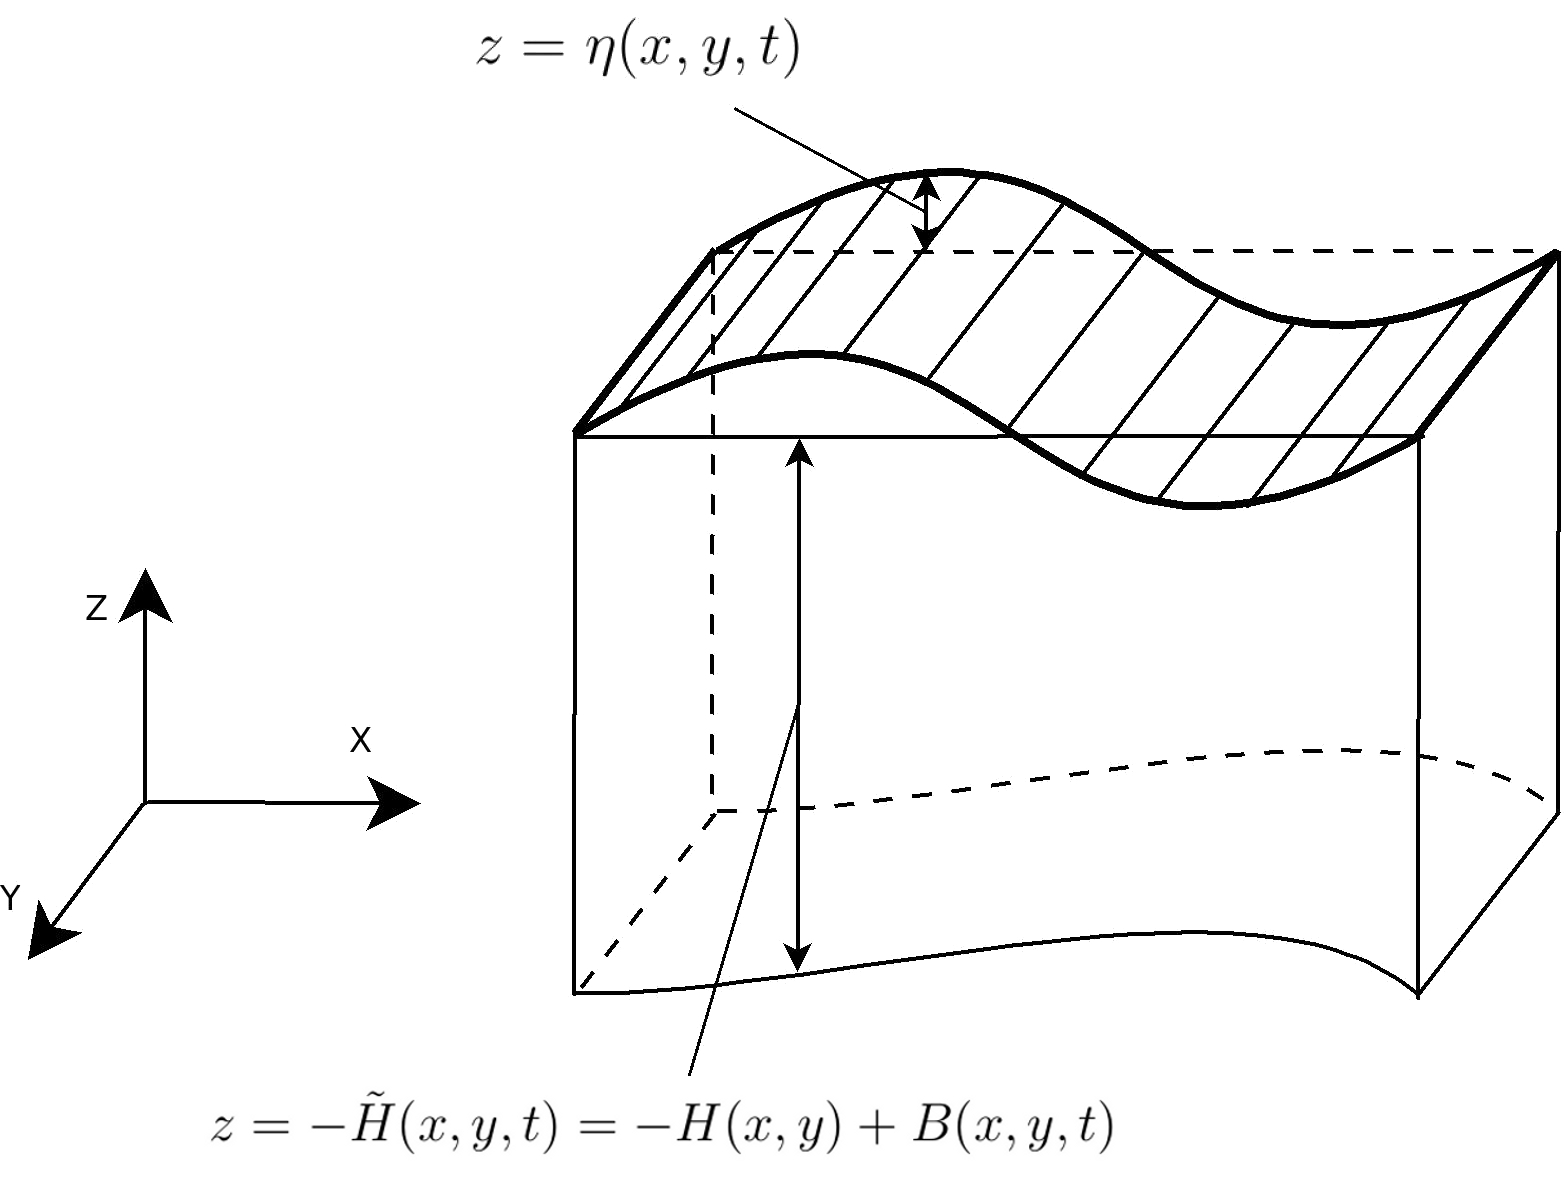
\includegraphics[width=9cm,height=6cm]{scheme.jpg}
    \caption{Постановка задачи}
    \label{figure:schema}
\end{figure}

В качестве физической модели, описывающей данную задачу, взяты уравнения теории мелкой воды (в линейной форме известные также как уравнения Сен-Венана), для которых существенными являются предположения о малости вертикального ускорения частиц жидкости по отношению к ускорению свободного падения и о слабой зависимости горизонтальных скоростей от вертикальной координаты.

Ситуации, когда глубина акватории много меньше горизонтальных размеров, достаточно обычна, поэтому уравнения мелкой воды находят широкое применение. Часто они используются с учётом кориолисовых сил при моделировании атмосферы и океана как упрощение системы примитивных уравнений, описывающих потоки в атмосфере.

Представим уравнения мелкой воды в следующей форме:
\begin{gather}
    \label{eq:MainVectorForm}
    \frac{\partial U}{\partial t}+F_{lin}+F_{nonlin}=\frac{\partial B}{\partial t}\\
    \label{eq:UB}
    U=\begin{pmatrix}\eta\\u\\v\end{pmatrix}
    B=\begin{pmatrix}B(x,y,t)\\0\\0\end{pmatrix}\notag
\end{gather}

\begin{gather}
    \label{eq:FLin}
    F_{lin}=\begin{pmatrix}
	\frac{\partial ((H-B)u)}{\partial x}+\frac{\partial ((H-B)v)}{\partial y}\\
	g\frac{\partial \eta}{\partial x}\\
	g\frac{\partial \eta}{\partial y}
    \end{pmatrix}\\
    \label{eq:FNonLin}
    F_{nonlin}=\begin{pmatrix}
	0\\
	\frac{1}{2}\frac{\partial (u^2)}{\partial x} + v\frac{\partial u}{\partial y}\\
	\frac{1}{2}\frac{\partial (v^2)}{\partial y} + u\frac{\partial v}{\partial x}
    \end{pmatrix}
\end{gather}

%Boundary
\begin{gather}
    \begin{split}
	\label{eq:BoundaryCondition}
	(x,y)&\in\Omega,t>0\\
	u_0=u(x,y,0)\;v_0=&v(x,y,0)\;\eta_0=\eta(x,y,0)\\
	u(x,y,t),v(x,y,t),\eta(&x,y,t)\to0\; x^2+y^2\to\infty
    \end{split}
\end{gather}

	Где $H$ определяет неподвижную часть дна, а $B$ - его динамическую составляющую ($H-B$ – полная грубина слоя жидкости), $\eta$ – функция свободной поверхности, $u(x,y,t)$ – скорость по Ox, $v(x,y,t)$ - скорость по Oy, $g=9,8$. 

	Данные формулы являются гиперболической системой дифференциальных уравнений и описывают более общую постановку задачи в нелинейном виде без учёта сил Кориолиса, трения и вязкости в бесконечной области (более подробно об уравнениях мелкой воды см. \cite{ovsjannikov},\cite{marchyk}). Линейная форма может быть получена как частный случай - для этого достаточно отбросить $F_{nonlin}$.

\newpage
\addtocounter{section}{1}
\setcounter{subsection}{0}
\setcounter{equation}{0}
\section*{Аппроксимация уравнений}
\addtocontents{toc}{\contentsline{section}{\protect\numberline{\S\;\thesection.}\vspace{10pt}Аппроксимация уравнений}{\thepage}}

Задача (\ref{eq:MainVectorForm}), (\ref{eq:BoundaryCondition}) решалась методом сеток. Для решения в расчетной области $\Omega$ введем обычным образом неравномерную в общем случае сетку $\Omega_h$ с шагом $h_{x i}=x_{i+1}-x_{i},h_{y i}=y_{i+1}-y_{i}$ и шагом по времени $\tau=t^{n+1}-t^n$. $n$-й слой по времени определим как множество узлов $(i,j)$ при фиксированном $t^n$.

Обозначим значение сеточной функции $\phi$ в узле $(i,j)$, как $\phi^n_{ij}=\phi(x_i,y_i,t^n)$ и аппроксимируем уравнения (\ref{eq:MainVectorForm}), (\ref{eq:BoundaryCondition}) в узлах сетки $\Omega_h$ на $n$-м слое неявной конечно-разностной схемой второго порядка аппроксимации:

\begin{eqnarray}
    \label{eq:ApproxMainEq}
    \frac{U_{ij}^{n+1}-U_{ij}^{n}}{\tau}+F^{n+1}_{lin}+F^{n+1}_{nonlin}=\frac{B_{ij}^{n+1}-B_{ij}^{n}}{\tau}
\end{eqnarray}

\begin{eqnarray}
    \label{eq:ApproxFLin}
    F^{n+1}_{lin}=\begin{pmatrix}
	\frac{(H_{i+1j}-B_{i+1j}^{n+1})u_{i+1j}^{n+1}-(H_{i-1j}-B_{i-1j}^{n+1})u_{i-1j}^{n+1}}{2h_x}+\\
	\frac{(H_{ij+1}-B_{ij+1}^{n+1})v_{ij+1}^{n+1}-(H_{ij-1}-B_{ij-1}^{n+1})v_{ij-1}^{n+1}}{2h_y}\\
	\frac{u_{ij}^{n+1}-u_{ij}^{n}}{\tau}+
	g\frac{\eta_{i+1j}^{n+1}-\eta_{i-1j}^{n+1}}{2h_x}\\
	\frac{v_{ij}^{n+1}-v_{ij}^{n}}{\tau}+
	g\frac{\eta_{ij+1}^{n+1}-\eta_{ij-1}^{n+1}}{2h_y}
    \end{pmatrix}
\end{eqnarray}

\begin{eqnarray}
    \label{eq:ApproxFNonlin}
    F^{n+1}_{nonlin}=\begin{pmatrix}
	0\\
	v_{ij}\frac{u_{ij+1}^{n+1}-u_{ij-1}^{n}}{2h_y}+
	\frac{(u_{i+1j}^{n+1})^2-(u_{i-1j}^{n})^2}{2h_x}\\
	u_{ij}\frac{v_{i+1j}^{n+1}-v_{i-1j}^{n}}{2h_x}+
	\frac{(v_{ij+1}^{n+1})^2-(v_{ij-1}^{n})^2}{2h_y}
    \end{pmatrix}
\end{eqnarray}

\begin{gather}
    \begin{split}
	\label{eq:BeginValues}
	u_{ij}^0=u_0(x_i,y_i)\;
	v_{ij}^0=v_0(x_i,y_i)\;
	\eta_{ij}^0=\eta_0(x_i,y_i)
    \end{split}
\end{gather}

\begin{gather*}
    n=0,1 \ldots N \; i,j=0,\pm 1,\pm 2 \ldots
\end{gather*}

где $H_{i,j}=H(x_i,y_j)$, $B_{i,j,n}=B(x_i,y_i,t^n)$ - постоянная и динамическая составляющие функции дна.

Принято считать, что в неявной схеме можно без потери точности вычислений брать шаг по $t$ гораздо большим, чем в явной, и этим существенно поднять скорость вычислений или повысить точность. Кроме того, подобные схемы оптимально подходят для задач на установление, когда вместо решения уравнения $AX=0$ шагами по времени ищут состояние покоя системы $\frac{dX}{dt}=AX$, наступающее в отдаленном времени.

\newpage
\addtocounter{section}{1}
\setcounter{subsection}{0}
\setcounter{equation}{0}
\section*{Выбор граничных условий}
\addtocontents{toc}{\contentsline{section}{\protect\numberline{\S\;\thesection.}\vspace{10pt}Выбор граничных условий}{\thepage}}

Для численного решения задачи (\ref{eq:MainVectorForm}), (\ref{eq:BoundaryCondition}) необходимо ограничить расчетную область. Основной проблемой при этом является поиск таких условий на искусственных границах, которые не приводят к отражениям или искажениям волны, проходящей через границу (так называемых, «прозрачных» или «неотражающих» краевых условий).

Как известно (см. \cite{ilgamov}, \cite{ryabenky}) существуют способы задания искусcтвенных краевых условий которые в некоторых случаях позволяют выходить волнам из $Q$ без отражений и искажений.

\addtocounter{subsection}{1}
\subsection*{Виды неотражающих краевых условий}
\addtocontents{toc}{\contentsline{subsection}{\protect\numberline{\thesubsection.}\vspace{10pt}Виды неотражающих краевых условий}{\thepage}}
В кратце опишем существующие виды прозрачных краевых условий:
\begin{itemize}
    \item Неотражающие граничные условия

	Основная идея постановки неотражающих граничных условий заключается в нахождении решения системы и представления его в виде суперпозиции разнонаправленных волн. Исходя из этого на границе ставятся такие условия, которые уничтожают ненужные волны (пример такой постановки условий \cite{mcdonald}).

    \item Поглощающие граничные условия

	Основная идея постановки поглощающих граничных условий -  окружить расчетную область поглощающим слоем конечной ширины. В результате все волны должны попадать в этот слой и поглощаться независимо от частоты и угла падения(пример такой постановки условий \cite{pml}).
\end{itemize}

\addtocounter{subsection}{1}
\subsection*{Замыкание системы уравнений}
\addtocontents{toc}{\contentsline{subsection}{\protect\numberline{\thesubsection.}\vspace{10pt}Замыкание системы уравнений}{\thepage}}

К сожалению, указанные выше методы оказались недостаточно гибкими и содержали множество ограничений. Например, для постановки неотражающих условий необходимо иметь точное решение системы уравнений, которое для нелинейных уравнений нельзя найти в общем случае. Постановка поглощающих граничных условий же черевата неустойчивостью полученного решения на длительных промежутках времени. В результате был предложен следующий способ.

Т.к. искусственные границы принадлежат расчетной области и тем самым на них выполняются уравнения теории мелкой воды, то для замыкания схемы (\ref{eq:ApproxMainEq})-(\ref{eq:ApproxFNonlin}) на границах и в углах можно произвести аппроксимацию этих уравнений внутрь рассчетной области. В итоге получим замкнутую систему уравнений, которую и будем решать.

Т.о. аппроксимация на границе $\Gamma=\Gamma_1\cup \Gamma_2\cup \Gamma_3\cup \Gamma_4$ расчетной области выглядит следующим образом:

\begin{figure}[htp]
    \centering
    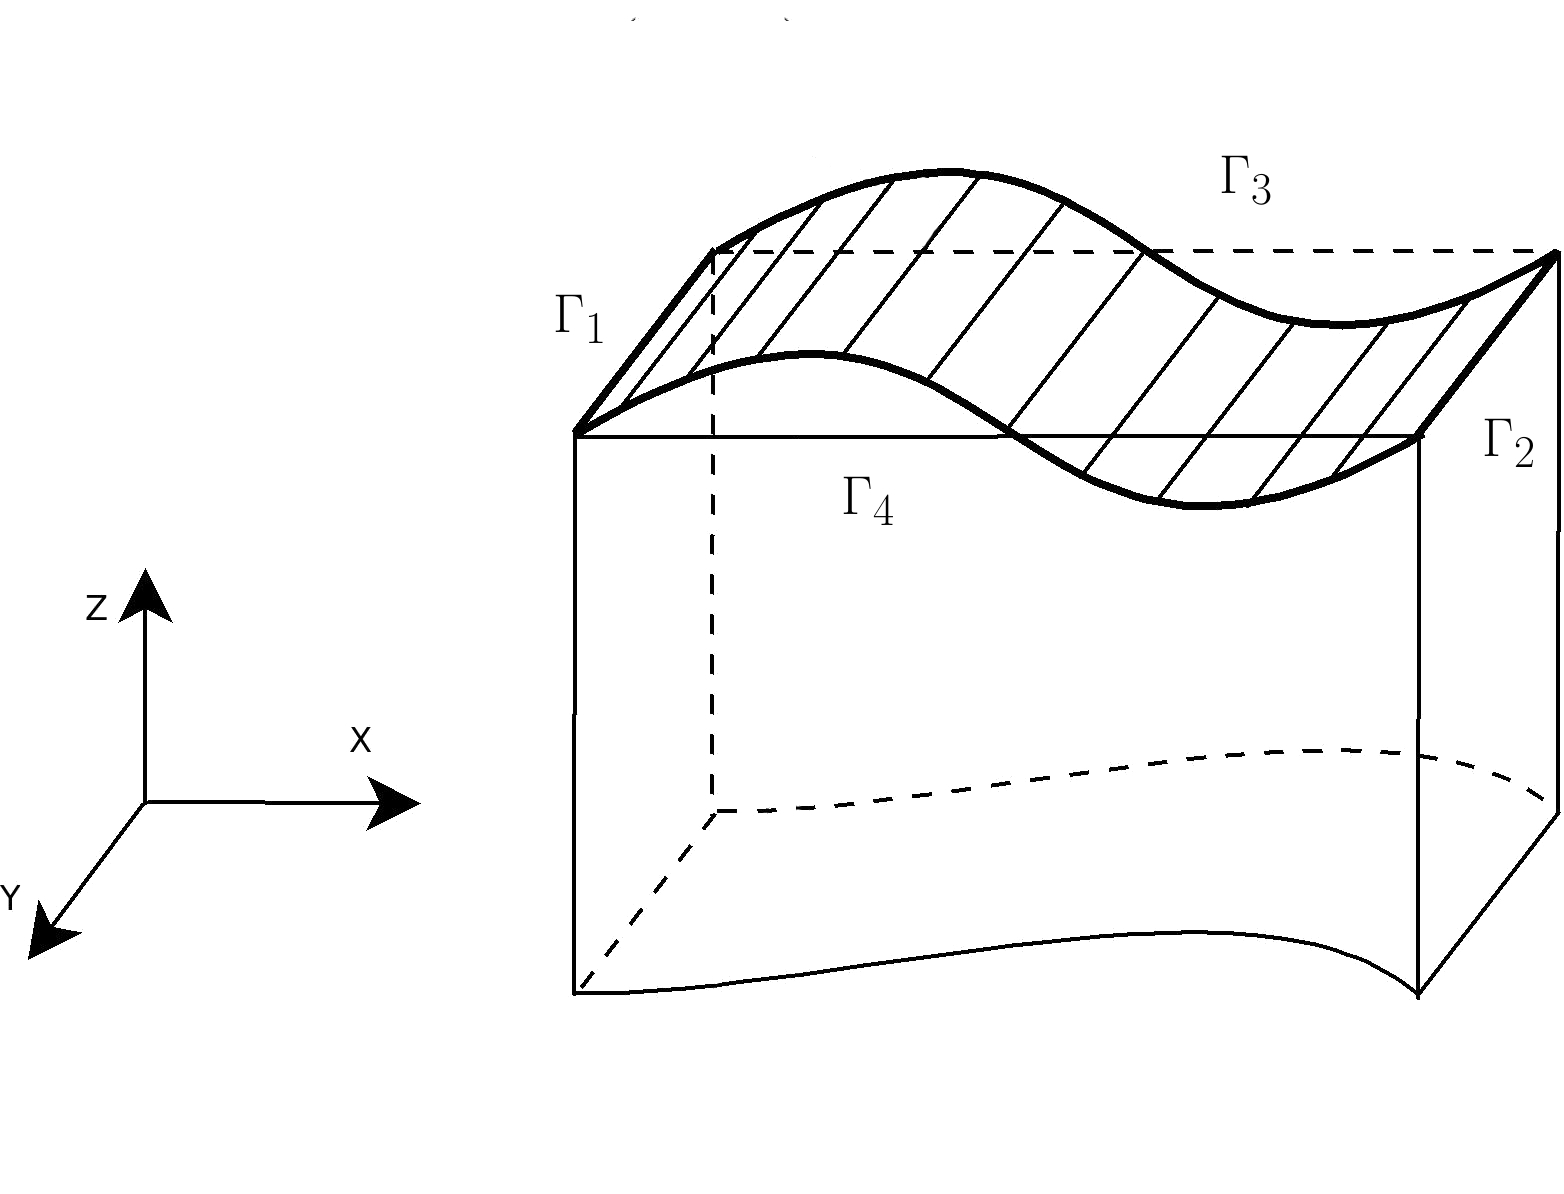
\includegraphics[width=9cm,height=6cm]{boundary_scheme.jpg}
    \caption{Искусственные границы}
    \label{figure:boundary_schema}
\end{figure}

\begin{itemize}

    \item На границе $\Gamma_1=\{x=0,y\in[0,1]\}$
	\begin{eqnarray}
	    \label{eq:ApproxFLinGamma1}
	    F^{n+1}_{lin}=\begin{pmatrix}
		\frac{(H_{1j}-B_{1j}^{n+1})u_{1j}^{n+1}-(H_{0j}-B_{0j}^{n+1})u_{0j}^{n+1}}{2h_x}+\\
		\frac{(H_{0j+1}-B_{0j+1}^{n+1})v_{0j+1}^{n+1}-(H_{0j-1}-B_{0j-1}^{n+1})v_{0j-1}^{n+1}}{2h_y}\\
		\frac{u_{0j}^{n+1}-u_{0j}^{n}}{\tau}+
		g\frac{\eta_{1j}^{n+1}-\eta_{0j}^{n+1}}{2h_x}\\
		\frac{v_{0j}^{n+1}-v_{0j}^{n}}{\tau}+
		g\frac{\eta_{0j+1}^{n+1}-\eta_{0j-1}^{n+1}}{2h_y}
	    \end{pmatrix}
	\end{eqnarray}

	\begin{eqnarray}
	    \label{eq:ApproxFNonlinGamma1}
	    F^{n+1}_{nonlin}=\begin{pmatrix}
		0\\
		v_{0j}\frac{u_{0j+1}^{n+1}-u_{0j-1}^{n}}{2h_y}+
		\frac{(u_{1j}^{n+1})^2-(u_{0j}^{n})^2}{2h_x}\\
		u_{0j}\frac{v_{1j}^{n+1}-v_{0j}^{n}}{2h_x}+
		\frac{(v_{0j+1}^{n+1})^2-(v_{0j-1}^{n})^2}{2h_y}
	    \end{pmatrix}
	\end{eqnarray}

    \item На границе $\Gamma_2=\{x=1,y\in[0,1]\}$
	\begin{eqnarray}
	    \label{eq:ApproxFLinGamma2}
	    F^{n+1}_{lin}=\begin{pmatrix}
		\frac{(H_{n_{x}j}-B_{n_{x}j}^{n+1})u_{n_{x}j}^{n+1}-(H_{n_{x}-1j}-B_{n_{x}-1j}^{n+1})u_{n_{x}-1j}^{n+1}}{2h_x}+\\
		\frac{(H_{n_{x}j+1}-B_{n_{x}j+1}^{n+1})v_{n_{x}j+1}^{n+1}-(H_{n_{x}j-1}-B_{n_{x}j-1}^{n+1})v_{n_{x}j-1}^{n+1}}{2h_y}\\
		\frac{u_{n_{x}j}^{n+1}-u_{n_{x}j}^{n}}{\tau}+
		g\frac{\eta_{n_{x}j}^{n+1}-\eta_{n_{x}-1j}^{n+1}}{2h_x}\\
		\frac{v_{n_{x}j}^{n+1}-v_{n_{x}j}^{n}}{\tau}+
		g\frac{\eta_{n_{x}j+1}^{n+1}-\eta_{n_{x}j-1}^{n+1}}{2h_y}
	    \end{pmatrix}
	\end{eqnarray}

	\begin{eqnarray}
	    \label{eq:ApproxFNonlinGamma2}
	    F^{n+1}_{nonlin}=\begin{pmatrix}
		0\\
		v_{n_{x}j}\frac{u_{n_{x}j+1}^{n+1}-u_{n_{x}j-1}^{n}}{2h_y}+
		\frac{(u_{n_{x}j}^{n+1})^2-(u_{n_{x}-1j}^{n})^2}{2h_x}\\
		u_{n_{x}j}\frac{v_{n_{x}j}^{n+1}-v_{n_{x}-1j}^{n}}{2h_x}+
		\frac{(v_{n_{x}j+1}^{n+1})^2-(v_{n_{x}j-1}^{n})^2}{2h_y}
	    \end{pmatrix}
	\end{eqnarray}

    \item На границе $\Gamma_3=\{x=\in[0,1],y=0\}$
	\begin{eqnarray}
	    \label{eq:ApproxFLinGamma3}
	    F^{n+1}_{lin}=\begin{pmatrix}
		\frac{(H_{i+10}-B_{i+10}^{n+1})u_{i+10}^{n+1}-(H_{i-10}-B_{i-10}^{n+1})u_{i-10}^{n+1}}{2h_x}+\\
		\frac{(H_{i1}-B_{i1}^{n+1})v_{i1}^{n+1}-(H_{i0}-B_{i0}^{n+1})v_{i0}^{n+1}}{2h_y}\\
		\frac{u_{i0}^{n+1}-u_{i0}^{n}}{\tau}+
		g\frac{\eta_{i+10}^{n+1}-\eta_{i-10}^{n+1}}{2h_x}\\
		\frac{v_{i0}^{n+1}-v_{i0}^{n}}{\tau}+
		g\frac{\eta_{i1}^{n+1}-\eta_{i0}^{n+1}}{2h_y}
	    \end{pmatrix}
	\end{eqnarray}

	\begin{eqnarray}
	    \label{eq:ApproxFNonlinGamma3}
	    F^{n+1}_{nonlin}=\begin{pmatrix}
		0\\
		v_{i0}\frac{u_{i1}^{n+1}-u_{i0}^{n}}{2h_y}+
		\frac{(u_{i+10}^{n+1})^2-(u_{i-10}^{n})^2}{2h_x}\\
		u_{i0}\frac{v_{i+10}^{n+1}-v_{i-10}^{n}}{2h_x}+
		\frac{(v_{i1}^{n+1})^2-(v_{i0}^{n})^2}{2h_y}
	    \end{pmatrix}
	\end{eqnarray}

    \item На границе $\Gamma_4=\{x=\in[0,1],y=1\}$
	\begin{eqnarray}
	    \label{eq:ApproxFLinGamma4}
	    F^{n+1}_{lin}=\begin{pmatrix}
		\frac{(H_{i+1n_{y}}-B_{i+1n_{y}}^{n+1})u_{i+1n_{y}}^{n+1}-(H_{i-1n_{y}}-B_{i-1n_{y}}^{n+1})u_{i-1n_{y}}^{n+1}}{2h_x}+\\
		\frac{(H_{in_{y}}-B_{in_{y}}^{n+1})v_{in_{y}}^{n+1}-(H_{in_{y}-1}-B_{in_{y}-1}^{n+1})v_{in_{y}-1}^{n+1}}{2h_y}\\
		\frac{u_{in_{y}}^{n+1}-u_{in_{y}}^{n}}{\tau}+
		g\frac{\eta_{i+1n_{y}}^{n+1}-\eta_{i-1n_{y}}^{n+1}}{2h_x}\\
		\frac{v_{in_{y}}^{n+1}-v_{in_{y}}^{n}}{\tau}+
		g\frac{\eta_{in_{y}}^{n+1}-\eta_{in_{y}-1}^{n+1}}{2h_y}
	    \end{pmatrix}
	\end{eqnarray}

	\begin{eqnarray}
	    \label{eq:ApproxFNonlinGamma4}
	    F^{n+1}_{nonlin}=\begin{pmatrix}
		0\\
		v_{in_{y}}\frac{u_{in_{y}}^{n+1}-u_{in_{y}-1}^{n}}{2h_y}+
		\frac{(u_{i+1n_{y}}^{n+1})^2-(u_{i-1n_{y}}^{n})^2}{2h_x}\\
		u_{in_{y}}\frac{v_{i+1n_{y}}^{n+1}-v_{i-1n_{y}}^{n}}{2h_x}+
		\frac{(v_{in_{y}}^{n+1})^2-(v_{in_{y}-1}^{n})^2}{2h_y}
	    \end{pmatrix}
	\end{eqnarray}

\end{itemize}

Аппроксимация в углах расчетной области выглядит следующим образом:

\begin{itemize}

    \item $x=0\;y=0$
	\begin{eqnarray*}
	    F^{n+1}_{lin}=\begin{pmatrix}
		\frac{(H_{10}-B_{10}^{n+1})u_{10}^{n+1}-(H_{00}-B_{00}^{n+1})u_{00}^{n+1}}{2h_x}+\\
		\frac{(H_{01}-B_{01}^{n+1})v_{01}^{n+1}-(H_{00}-B_{00}^{n+1})v_{00}^{n+1}}{2h_y}\\
		\frac{u_{00}^{n+1}-u_{00}^{n}}{\tau}+
		g\frac{\eta_{10}^{n+1}-\eta_{00}^{n+1}}{2h_x}\\
		\frac{v_{00}^{n+1}-v_{00}^{n}}{\tau}+
		g\frac{\eta_{01}^{n+1}-\eta_{00}^{n+1}}{2h_y}
	    \end{pmatrix}
	\end{eqnarray*}

	\begin{eqnarray*}
	    F^{n+1}_{nonlin}=\begin{pmatrix}
		0\\
		v_{00}\frac{u_{01}^{n+1}-u_{00}^{n}}{2h_y}+
		\frac{(u_{10}^{n+1})^2-(u_{00}^{n})^2}{2h_x}\\
		u_{00}\frac{v_{10}^{n+1}-v_{00}^{n}}{2h_x}+
		\frac{(v_{01}^{n+1})^2-(v_{00}^{n})^2}{2h_y}
	    \end{pmatrix}
	\end{eqnarray*}

    \item $x=1\;y=0$
	\begin{eqnarray*}
	    F^{n+1}_{lin}=\begin{pmatrix}
		\frac{(H_{n_{x}0}-B_{n_{x}0}^{n+1})u_{n_{x}0}^{n+1}-(H_{n_{x}-10}-B_{n_{x}-10}^{n+1})u_{n_{x}-10}^{n+1}}{2h_x}+\\
		\frac{(H_{n_{x}1}-B_{n_{x}1}^{n+1})v_{n_{x}1}^{n+1}-(H_{n_{x}0}-B_{n_{x}0}^{n+1})v_{n_{x}0}^{n+1}}{2h_y}\\
		\frac{u_{n_{x}0}^{n+1}-u_{n_{x}0}^{n}}{\tau}+
		g\frac{\eta_{n_{x}0}^{n+1}-\eta_{n_{x}-10}^{n+1}}{2h_x}\\
		\frac{v_{n_{x}0}^{n+1}-v_{n_{x}0}^{n}}{\tau}+
		g\frac{\eta_{n_{x}1}^{n+1}-\eta_{n_{x}0}^{n+1}}{2h_y}
	    \end{pmatrix}
	\end{eqnarray*}

	\begin{eqnarray*}
	    F^{n+1}_{nonlin}=\begin{pmatrix}
		0\\
		v_{n_{x}0}\frac{u_{n_{x}1}^{n+1}-u_{n_{x}0}^{n}}{2h_y}+
		\frac{(u_{n_{x}0}^{n+1})^2-(u_{n_{x}-10}^{n})^2}{2h_x}\\
		u_{n_{x}0}\frac{v_{n_{x}0}^{n+1}-v_{n_{x}-10}^{n}}{2h_x}+
		\frac{(v_{n_{x}1}^{n+1})^2-(v_{n_{x}0}^{n})^2}{2h_y}
	    \end{pmatrix}
	\end{eqnarray*}

    \item $x=0\;y=1$
	\begin{eqnarray*}
	    F^{n+1}_{lin}=\begin{pmatrix}
		\frac{(H_{1n_{y}}-B_{1n_{y}}^{n+1})u_{1n_{y}}^{n+1}-(H_{0n_{y}}-B_{0n_{y}}^{n+1})u_{0n_{y}}^{n+1}}{2h_x}+\\
		\frac{(H_{0n_{y}}-B_{0n_{y}}^{n+1})v_{0n_{y}}^{n+1}-(H_{0n_{y}-1}-B_{0n_{y}-1}^{n+1})v_{0n_{y}-1}^{n+1}}{2h_y}\\
		\frac{u_{0n_{y}}^{n+1}-u_{0n_{y}}^{n}}{\tau}+
		g\frac{\eta_{1n_{y}}^{n+1}-\eta_{0n_{y}}^{n+1}}{2h_x}\\
		\frac{v_{0n_{y}}^{n+1}-v_{0n_{y}}^{n}}{\tau}+
		g\frac{\eta_{0n_{y}}^{n+1}-\eta_{0n_{y}-1}^{n+1}}{2h_y}
	    \end{pmatrix}
	\end{eqnarray*}

	\begin{eqnarray*}
	    F^{n+1}_{nonlin}=\begin{pmatrix}
		0\\
		v_{0n_{y}}\frac{u_{0n_{y}}^{n+1}-u_{0n_{y}-1}^{n}}{2h_y}+
		\frac{(u_{1n_{y}}^{n+1})^2-(u_{0n_{y}}^{n})^2}{2h_x}\\
		u_{0n_{y}}\frac{v_{1n_{y}}^{n+1}-v_{0n_{y}}^{n}}{2h_x}+
		\frac{(v_{0n_{y}}^{n+1})^2-(v_{0n_{y}-1}^{n})^2}{2h_y}
	    \end{pmatrix}
	\end{eqnarray*}

    \item $x=1\;y=1$
	\begin{eqnarray*}
	    F^{n+1}_{lin}=\begin{pmatrix}
		\frac{(H_{n_{x}n_{y}}-B_{n_{x}n_{y}}^{n+1})u_{n_{x}n_{y}}^{n+1}-(H_{n_{x}-1n_{y}}-B_{n_{x}-1n_{y}}^{n+1})u_{n_{x}-1n_{y}}^{n+1}}{2h_x}+\\
		\frac{(H_{n_{x}n_{y}}-B_{n_{x}n_{y}}^{n+1})v_{n_{x}n_{y}}^{n+1}-(H_{n_{x}n_{y}-1}-B_{n_{x}n_{y}-1}^{n+1})v_{n_{x}n_{y}-1}^{n+1}}{2h_y}\\
		\frac{u_{n_{x}n_{y}}^{n+1}-u_{n_{x}n_{y}}^{n}}{\tau}+
		g\frac{\eta_{n_{x}n_{y}}^{n+1}-\eta_{n_{x}-1n_{y}}^{n+1}}{2h_x}\\
		\frac{v_{n_{x}n_{y}}^{n+1}-v_{n_{x}n_{y}}^{n}}{\tau}+
		g\frac{\eta_{n_{x}n_{y}}^{n+1}-\eta_{n_{x}n_{y}-1}^{n+1}}{2h_y}
	    \end{pmatrix}
	\end{eqnarray*}

	\begin{eqnarray*}
	    F^{n+1}_{nonlin}=\begin{pmatrix}
		0\\
		v_{ij}\frac{u_{ij+1}^{n+1}-u_{ij-1}^{n}}{2h_y}+
		\frac{(u_{i+1j}^{n+1})^2-(u_{i-1j}^{n})^2}{2h_x}\\
		u_{ij}\frac{v_{i+1j}^{n+1}-v_{i-1j}^{n}}{2h_x}+
		\frac{(v_{ij+1}^{n+1})^2-(v_{ij-1}^{n})^2}{2h_y}
	    \end{pmatrix}
	\end{eqnarray*}

\end{itemize}

\newpage
\addtocounter{section}{1}
\setcounter{subsection}{0}
\setcounter{equation}{0}
\section*{Алгоритм решения}
\addtocontents{toc}{\contentsline{section}{\protect\numberline{\S\;\thesection.}\vspace{10pt}Алгоритм решения}{\thepage}}

В итоге, схема (\ref{eq:ApproxMainEq})-(\ref{eq:ApproxFNonlin}) с замыканием на $\Gamma$ представляет собой систему нелинейных алгебраических уравнений (СНАУ)

\begin{gather}
    AU=f\notag\\
    A=A_{lin}+A_{nonlin}
    \label{eq:MainSolveEq}
\end{gather}
относительно переменных $U^n=(\eta^{n+1}_{00},\ldots,\eta^{n+1}_{n_xn_y},u^{n+1}_{00},\ldots,u^{n+1}_{n_xn_y},v^{n+1}_{00},\ldots,v^{n+1}_{n_xn_y0})$, где вектор $f$ известен и зависит от $\eta^{n+1}_{ij},u^{n+1}_{ij},v^{n+1}_{ij},H_{ij},B^{n+1}_{ij},B^{n}_{ij}$, а $A_{lin}$ - оператор аппроксимации линейной части (\ref{eq:MainVectorForm})-(\ref{eq:BoundaryCondition}), $A_{nonlin}$ - оператор аппроксимации нелинейной части (\ref{eq:MainVectorForm})-(\ref{eq:BoundaryCondition}).

Для решения задачи (\ref{eq:MainVectorForm})-(\ref{eq:BoundaryCondition}) использовался следующий алгоритм:
\begin{itemize}
    \item По известному вектору $\{u_{ij}^n,v_{ij}^n,\eta_{ij}^n\}$ на каждом временном слое каким-либо итерационным методом находим приближенное решение системы (\ref{eq:MainSolveEq}).
    \item Оно принимается за решение схемы (\ref{eq:ApproxMainEq})-(\ref{eq:ApproxFNonlin}) на n+1 слое.
\end{itemize}

Матрица полученной системы уравнений не обладает свойствами, необходимыми для решения системы известными методами, поэтому для ее решения мы воспользовались методом неполной аппроксимации минимальных невязок, шаг которого выглядит следующим образом:

\begin{equation}
    \label{FirstMethodStep}
    u^{k+\frac{1}{2}}=u^k-\tau_{k+1}r^k\\
\end{equation}
\begin{equation}
    \label{SecondMethodStep}
    u^{k+1}=u^{k+\frac{1}{2}}-\alpha_{k+1}z^k
\end{equation}

где $\tau$ - итерационный параметр, выбираемый из условия минимума $\|r^{k+\frac{1}{2}}\|$,$z^k$ - заданный вектор,$\alpha$ - матрица итерационных параметров, элементы которой выбираются из минимума последовательности норм невязок.

\newpage
\addtocounter{section}{1}
\setcounter{subsection}{0}
\setcounter{equation}{0}
\section*{Описание двухслойной схемы неполной аппроксимации}
\addtocontents{toc}{\contentsline{section}{\protect\numberline{\S\;\thesection.}\vspace{10pt}Описание двухслойной схемы неполной аппроксимации}{\thepage}}

Пусть в конечномерном вещественном гильбертовом пространстве $H_m$ задана система уравнений
\begin{equation}
    \label{eq:MainMethodSystem}
    Au=f
\end{equation}
с невырожденной незнакоопределенной матрицей $A=(a_{ij})$ порядка $m$. Здесь $u,f$ - неизвестный и известный $m$-мерные векторы из $H_m$.

В дальнейшем будем считать, что $det A$ или одно из собственных чисел могут быть близкими к машинному нулю. Если матрица незнакоопределена, то, умножая систему (\ref{eq:MainMethodSystem}) на $A^*$ (1-ая трансформация Гаусса), получим новую систему с положительно определенной матрицей $\overline{A}=A^{*}A$ и правой частью $A^{*}f$. Для решения этой системы можно использовать достаточно широкий арсенал итерационных схем, но в нашем случае такой путь решения системы (\ref{eq:MainMethodSystem}) не приемлем, т.к. $det A$ или одно из собственных чисел могут быть близкими к машинному нулю.

Для решения системы (\ref{eq:MainMethodSystem}) рассмотрим итерационную схему неполной аппроксимации (более подробное описание метода см. \cite{zakharov})
\begin{equation}
    \label{eq:FirstTheoryMethodStep}
    u^{n+\frac{1}{2}}=u^n-\tau_{n+1}B(Au^n-f)\\
\end{equation}
\begin{equation}
    \label{eq:SecondTheoryMethodStep}
    u^{n+1}=u^{n+\frac{1}{2}}-\alpha_{n+1}z^n,\;n=0,1,2,\ldots
\end{equation}
где $B$ - неособенная квадратная матрица, $z^n\in H_m$ - произвольный вектор, $\tau_{n+1},\alpha_{n+1}$ -итерационные параметры, $u^0$ - произвольный начальный вектор. Заметим, что $\alpha_{n+1}$ может быть как константой, так и матрицей.

\addtocounter{subsection}{1}
\subsection*{Случай, когда $\alpha_{n+1}=const$}
\addtocontents{toc}{\contentsline{subsection}{\protect\numberline{\thesubsection.}\vspace{10pt}Случай, когда $\alpha_{n+1}=const$}{\thepage}}

Пусть в схеме (\ref{eq:FirstTheoryMethodStep})-(\ref{eq:SecondTheoryMethodStep}) $\alpha_{n+1}=const$,а $D$ - самосопряженный положительно определенный оператор, дейтсвующий в $H_m$. Тогда относительно $v^n=D^{\frac{1}{2}}(u^n-u)$ система имеет вид

\begin{equation}
    \label{eq:FirstTheoryMethodStepResidual}
    v^{n+\frac{1}{2}}=S_{n+1}v^n\\
\end{equation}
\begin{equation}
    \label{eq:SecondTheoryMethodStepResidual}
    v^{n+1}=v^{n+\frac{1}{2}}-\alpha_{n+1}D^{\frac{1}{2}}z^n,\;n=0,1,2,\ldots
\end{equation}
где $S_{n+1}=E-\tau_{n+1}C,\; C=D^{\frac{1}{2}}z^n,\; v^{n+\frac{1}{2}}=D^{\frac{1}{2}}(u^{n+\frac{1}{2}}-u)$.

Тогда 
\begin{equation}
    \label{eq:TheoryMethodResidual1}
    \|v^{n+1}\|^2=\|v^{n+\frac{1}{2}}\|^2-2\alpha_{n+1}(v^{n+\frac{1}{2}},D^{\frac{1}{2}}z^n)+\alpha^2_{n+1}\|D^{\frac{1}{2}}z^n\|^2
\end{equation}

Если вектор $z^n$ такой, что $D^{\frac{1}{2}}z^n\neq 0$, то, выбирая $\alpha_{n+1}$ из условия минимума $\|v^{n+1}\|^2$, получаем
\begin{equation}
    \label{eq:TheoryMethodResidual2}
    \|v^{n+1}\|^2=\|v^{n+\frac{1}{2}}\|^2-\frac{(v^{n+\frac{1}{2}},D^{\frac{1}{2}}z^n)^2}{\|D^{\frac{1}{2}}z^n\|^2}
\end{equation}
при
\begin{equation}
    \label{eq:TheoryMethodAlpha}
    \alpha_{n+1}=\frac{(v^{n+\frac{1}{2}},D^{\frac{1}{2}}z^n)^2}{\|D^{\frac{1}{2}}z^n\|^2}
\end{equation}

Параметр $\tau_{n+1}$, например, можно выбирать из условия минимума $\|v^{n+\frac{1}{2}}\|^2$
\begin{equation}
    \label{eq:TheoryMethodResidual3}
    \|v^{n+\frac{1}{2}}\|^2=\|v^{n}\|^2-2\tau_{n+1}(v^{n},Cv^n)+\tau^2_{n+1}\|Cv^n\|^2
\end{equation}
тогда
\begin{equation}
    \label{eq:TheoryMethodTau}
    \tau_{n+1}=\frac{(Cv^{n},v^n)}{\|Cv^n\|^2}
\end{equation}
и формулу (\ref{eq:TheoryMethodResidual2}) можно пререписать в виде

\begin{equation}
    \label{eq:TheoryMethodResidualSimple}
    \|v^{n+1}\|^2=\Theta^{(1)}_{n+1}\|v^n\|^2
\end{equation}
где
\begin{equation}
    \label{eq:TheoryMethodResidualLessOne}
    \Theta^{(1)}_{n+1}=\rho^2_{n+1}-R_{n+1}\leq1
\end{equation}

\begin{equation}
    \label{eq:TheoryMethodResidualR}
    R_{n+1}=\frac{v^{n+\frac{1}{2}},D^{\frac{1}{2}}z^n)^2}{\|D^{\frac{1}{2}}z^n\|^2\|v^n\|^2}
\end{equation}

\begin{equation}
    \label{eq:TheoryMethodResidualRho}
    \rho^2_{n+1}=1-\frac{Cv^n,v^n)^2}{\|Cv^n\|^2\|v^n\|^2}
\end{equation}

Справедлива
\begin{Theorem}
    Если для всех $n$ вектор $z^n$ такой, что $(D^{\frac{1}{2}}v^{n+\frac{1}{2}},z^n)\neq 0$, то итерационная схема (\ref{eq:TheoryMethodResidual1}),\\(\ref{eq:TheoryMethodAlpha}),(\ref{eq:TheoryMethodTau}) сходится, т.е $\|v^{n+1}\|to 0$ при $n\to \infty$ для любого $v_0$
\end{Theorem}

В \cite{zakharov} показано, что строить векторы $z^n$ такие, чтобы для величины $\Theta^{(1)}_{n}$ выполнялась оценка $\Theta^{(1)}_{n}\leq\;\Theta_{*}<1$, достаточно просто.

\begin{Theorem}
    Итерационная схема (\ref{eq:TheoryMethodResidual1}),(\ref{eq:TheoryMethodAlpha}),(\ref{eq:TheoryMethodTau}) является сходящейся, если задать вектор $z^n$ в виде
    \begin{equation*}
	z^n=x^n+\frac{\sigma}{(D^{\frac{1}{2}}v^{\frac{1}{2}},v^{\frac{1}{2}})}v^{n+\frac{1}{2}}
    \end{equation*}
    со следующей оценкой:
    \begin{equation}
	\|v^{n+1}\|^2\leq(1-\xi)\rho^2_{n+1}\|v^n\|^2
    \end{equation}
    где $\xi = \frac{\gamma_1}{\gamma_2}$, a $\rho^2_{n+1}$ определяется равенством (\ref{eq:TheoryMethodResidualRho})
\end{Theorem}

\addtocounter{subsection}{1}
\subsection*{Случай, когда $\alpha_{n+1}$ является матрицей}
\addtocontents{toc}{\contentsline{subsection}{\protect\numberline{\thesubsection.}\vspace{10pt}Случай, когда $\alpha_{n+1}$ является матрицей}{\thepage}}

Для схемы (\ref{eq:FirstTheoryMethodStep})-(\ref{eq:SecondTheoryMethodStep}) введем параметр $\alpha_{n+1}$ в виде диагональной матрицы размерности $m$.

Пусть $z^n$ - вектор, все элементы которого равны единице, тогда произведение $\alpha_{n+1}z^n$ можно представить в виде
\begin{equation}
    \label{eq:AlphaZSumm}
    \alpha_{n+1}z^n=\sum^m_{i=1}\alpha^i_{n+1}z^n_i
\end{equation}
где $\alpha^i_{n+1}$ - элемент главной диагонали матрицы $a_{}n+1$, стоящий в $i$-й строке, $z^n_i$ - вектор с ненулевой $i$-й компонентой. Следовательно,

\begin{equation}
    \label{eq:VAlphaDZSumm}
    v^{n+1}=v^{n+\frac{1}{2}}-\sum^m_{i=1}\alpha^i_{n+1}D^{\frac{1}{2}}z^n_i
\end{equation}

Будем находить элементы матрицы $\{\alpha^i_{n+1}\}$ из условия минимума $\|v^{n+1}\|$
\begin{equation}
    \label{eq:MinNormaV}
    \|v^{n+1}\|^2=\|v^{n+\frac{1}{2}}\|^2-\sum^m_{i=1}\alpha^i_{n+1}(v^{n+\frac{1}{2}},D^{\frac{1}{2}}z^n_i)+\sum^m_{i=1}\sum^m_{j=1}\alpha^i_{n+1}\alpha^j_{n+1}(D^{\frac{1}{2}}z^n_i,D^{\frac{1}{2}}z^n_j)
\end{equation}

Для функций многих переменных справедлива
\begin{Theorem}
    Если $f(x)\in C^2(R^m)$, где $x\in R^m$, и выполнено условие
    \begin{equation}
	\frac{\partial f}{\partial x_i}(x_0)=0
    \end{equation}
    а также $d^2_{xx}f(x_0)$ - матрица частных производных второго порядка строго полодительно определена, то точка $x_0$ является точкой глобального минимума
\end{Theorem}

В \cite{zakharov} показано, что все условия теоремы выполняются, т.к. по условию матрица $D$ положительно определенная и неособенная, а векторы $\{z^n_m\}$ по построению линейно независимы.

\addtocounter{subsection}{1}
\subsection*{Метод минимальных невязок}
\addtocontents{toc}{\contentsline{subsection}{\protect\numberline{\thesubsection.}\vspace{10pt}Метод минимальных невязок}{\thepage}}

Пусть $D=A^*A$, тогда (\ref{eq:SecondTheoryMethodStepResidual}) перепишется в виде
\begin{equation}
    \label{eq:SecondTheoryMethodStepResidual2}
    v^{n+1}=v^{n+\frac{1}{2}}-\alpha_{n+1}(A^*A)^{\frac{1}{2}}z^n,\;n=0,1,2,\ldots
\end{equation}
и минимизируя $\|r^{n+1}\|$, получим

\begin{equation}
    \label{eq:TheoryMethodAlpha2}
    \alpha_{n+1}=\frac{(r^{n+\frac{1}{2}},Az^n)}{\|Az^n\|^2}
\end{equation}

Если же $\alpha_{n+1}$ - диагональная матрица, то ее элементы будем находить как решение системы
\begin{equation}
    \label{eq:TheoryMethodAlpha3}
    \begin{pmatrix}
	(Az^n_1,Az^n_1) & (Az^n_1,Az^n_2) & \cdots & (Az^n_1,Az^n_m)\\
	(Az^n_2,Az^n_1) & (Az^n_2,Az^n_2) & \cdots & (Az^n_2,Az^n_m)\\
	\vdots & \vdots & & \vdots\\
	(Az^n_m,Az^n_1) & (Az^n_m,Az^n_2) & \cdots & (Az^n_m,Az^n_m)\\
    \end{pmatrix}
    \times
    \begin{pmatrix}
	\alpha^1_{n+1}\\
	\alpha^2_{n+1}\\
	\vdots\\
	\alpha^m_{n+1}\\
    \end{pmatrix}
    =
    \begin{pmatrix}
	(Az^n_1,r^n)\\
	(Az^n_2,r^n)\\
	\vdots\\
	(Az^n_m,r^n)\\
    \end{pmatrix}\notag
\end{equation}


\newpage
\numberwithin{equation}{chapter}
\addtocounter{chapter}{1}
\setcounter{section}{0}
\setcounter{figure}{0}
\setcounter{table}{0}
\setcounter{equation}{0}
\diplomchapter*{Результаты расчетов}
\addtocontents{toc}{\contentsline{chapter}{\protect\numberline{Глава \thechapter.}\vspace{10pt}Результаты расчетов}{\thepage}}
В главе приведены результаты серии расчетов движения волн при различных  параметрах - например, шаг расчетной сетки, начальные данные, форма дна и т.д.

Для того, чтобы продемонстрировать пригодность метода решения, описанного в разделе \S1, проводились расчеты с разной начальной поверхностью и над разным дном. В них проверялось, насколько <<хорошо>> волна будет выходить из расчетной области, появятся ли искажения или отражения.

После этого проводились расчеты, направление на сравнение линейных ($F_{nonlin}=0$) и нелинейных ($F_{nonlin}\neq 0$) уравнений (\ref{eq:MainVectorForm}). Данные, полученные для линейного и нелинейного случая, анализировались и сравнивались, для выявления качественных различий. Для удобства восприятия, результаты обрабатывались отдельным модулем программы и визуализировались.

Помимо этого отдельно проводились расчеты для исследования явления <<возникновения волны>>.

Все расчеты представлены в двух проекциях - стандартной и вид сбоку. Сеточная поверхность, расположенная под свободной поверхностью - дно, над которым движется жидкость.

\newpage
\addtocounter{section}{1}
\setcounter{equation}{0}
\setcounter{subsection}{0}
\section*{Расчет со сложной начальной формой волны} 
\addtocontents{toc}{\contentsline{section}{\protect\numberline{\S\;\thesection.}\vspace{10pt}Расчет со сложной начальной формой волны}{\thepage}}

Рассмотрим задачу о движении начальной волны следующего вида:

$u_0=0\;v_0=0\;\eta_0=7 \cdot 10^{-3}e^{(-100 ((x-0.5)^2+(y-0.5)^2))}+4 \cdot 10^{-3}e^{(-300 ((x-0.7)^2+(y-0.7)^2))}$

в единичном квадрате глубиной $H(x,y)=10^{-2}$.

\begin{table}[H]
    \label{tab:FirstResult}
    \caption{Параметры для расчета со сложной формой поверхности}
    \begin{center}
	\begin{tabular}{|c|c|c|}
	    \hline
	    Размер области & $1\times1$\\
	    \hline
	    Количество шагов & $300$\\
	    \hline
	    Шаг по времени & $0.01$\\
	    \hline
	    Шаг сетки & $0.01$\\
	    \hline
	    Точность метода & $10^{-7}$\\
	    \hline
	    Форма дна & $H(x,y)=0.01\; B(x,y,t)=0$\\
	    \hline
	\end{tabular}
    \end{center}
\end{table}

На рис.\ref{fig:ComplexDrop} представлена динамика выхода волны из области решения.

\newpage
\begin{figure}[htp]
    \centering
    \vspace{12em}
    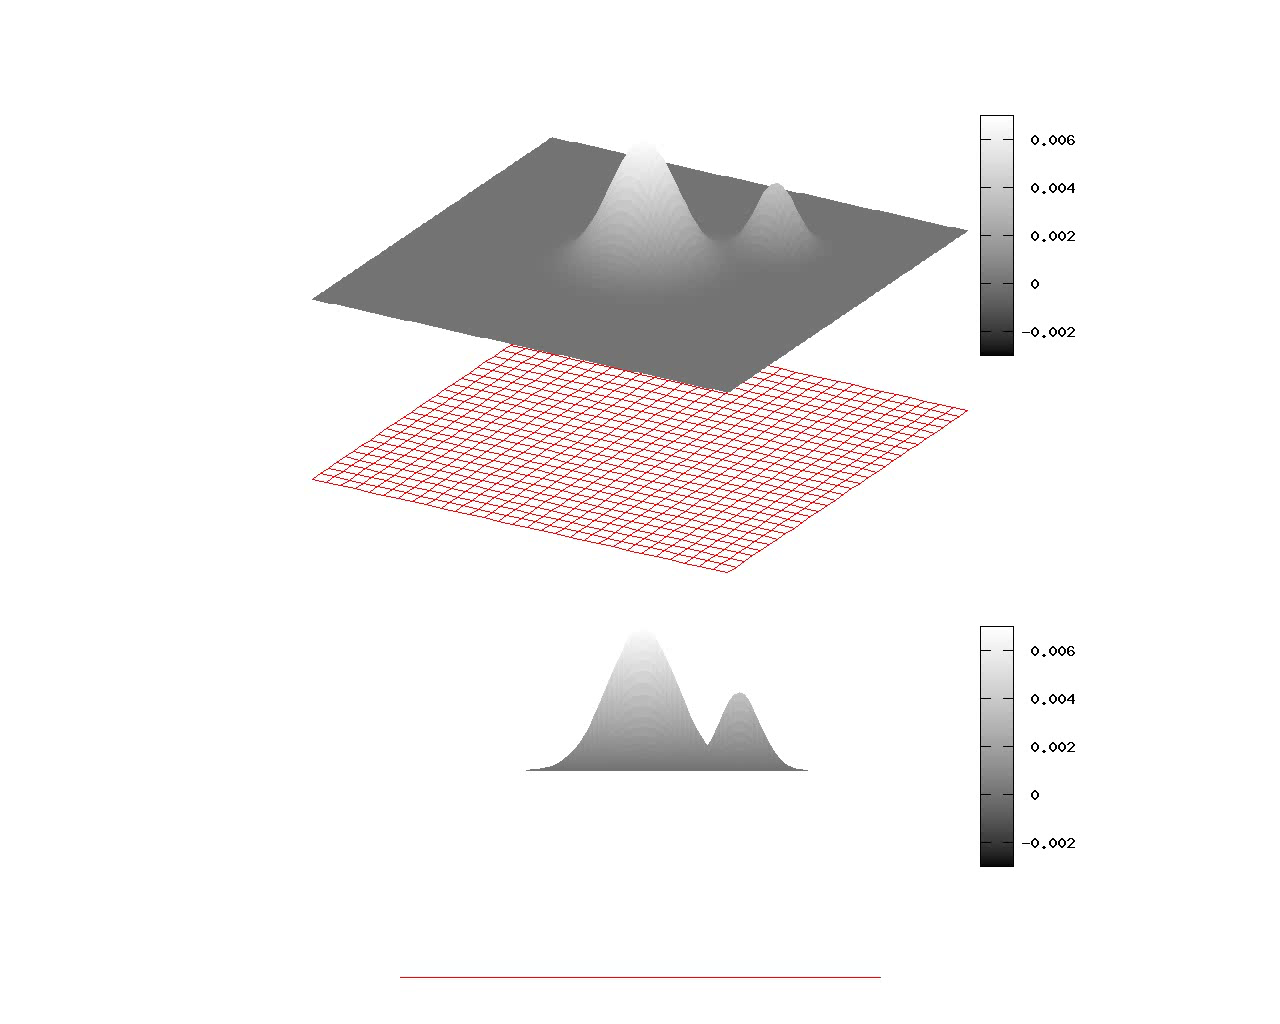
\includegraphics[width=8cm]{complex_drop1.png}
    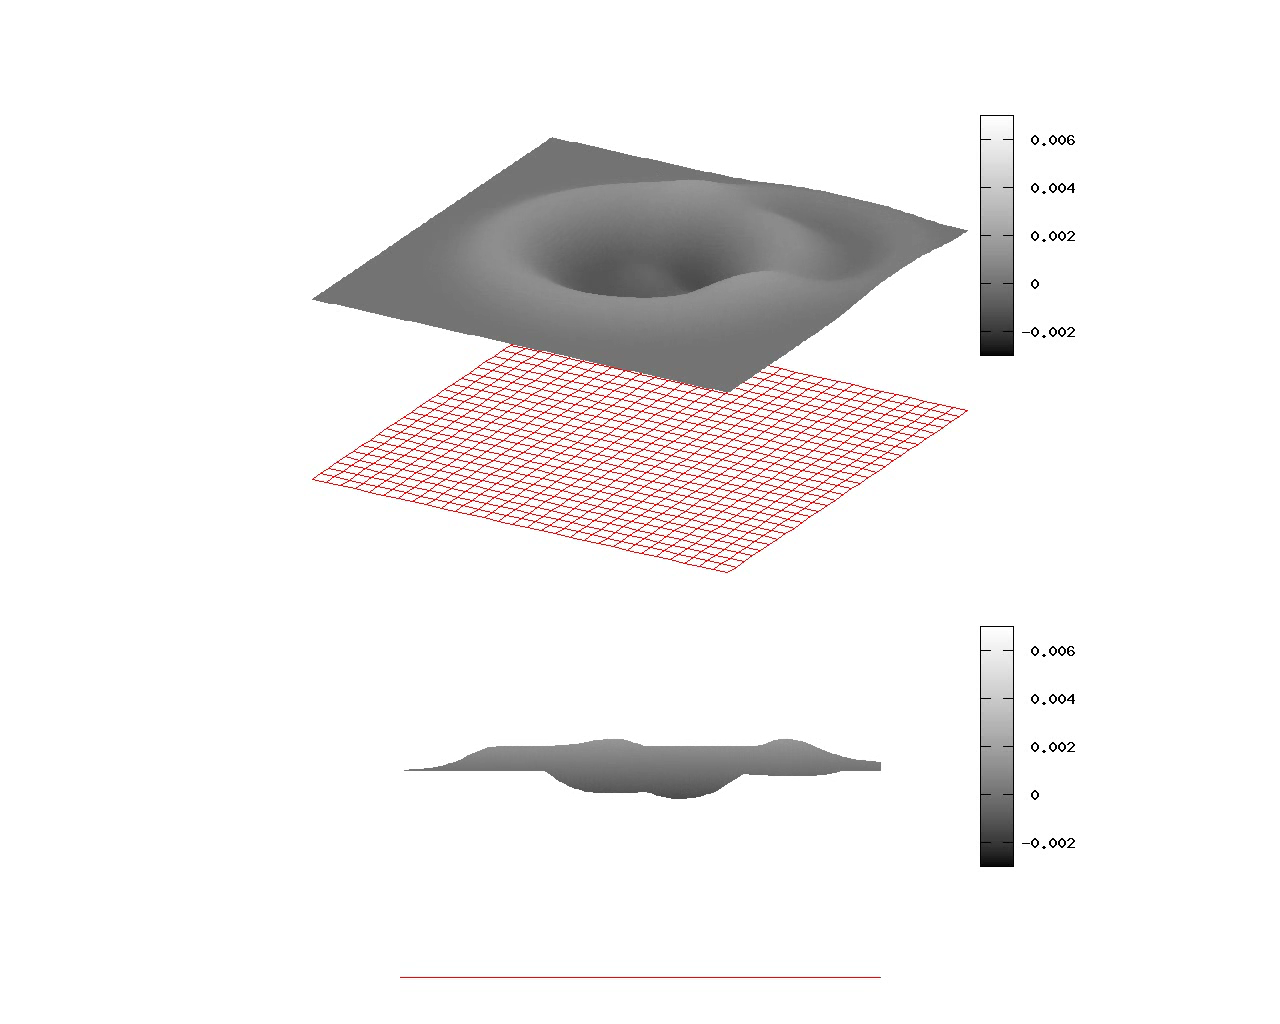
\includegraphics[width=8cm]{complex_drop2.png}
    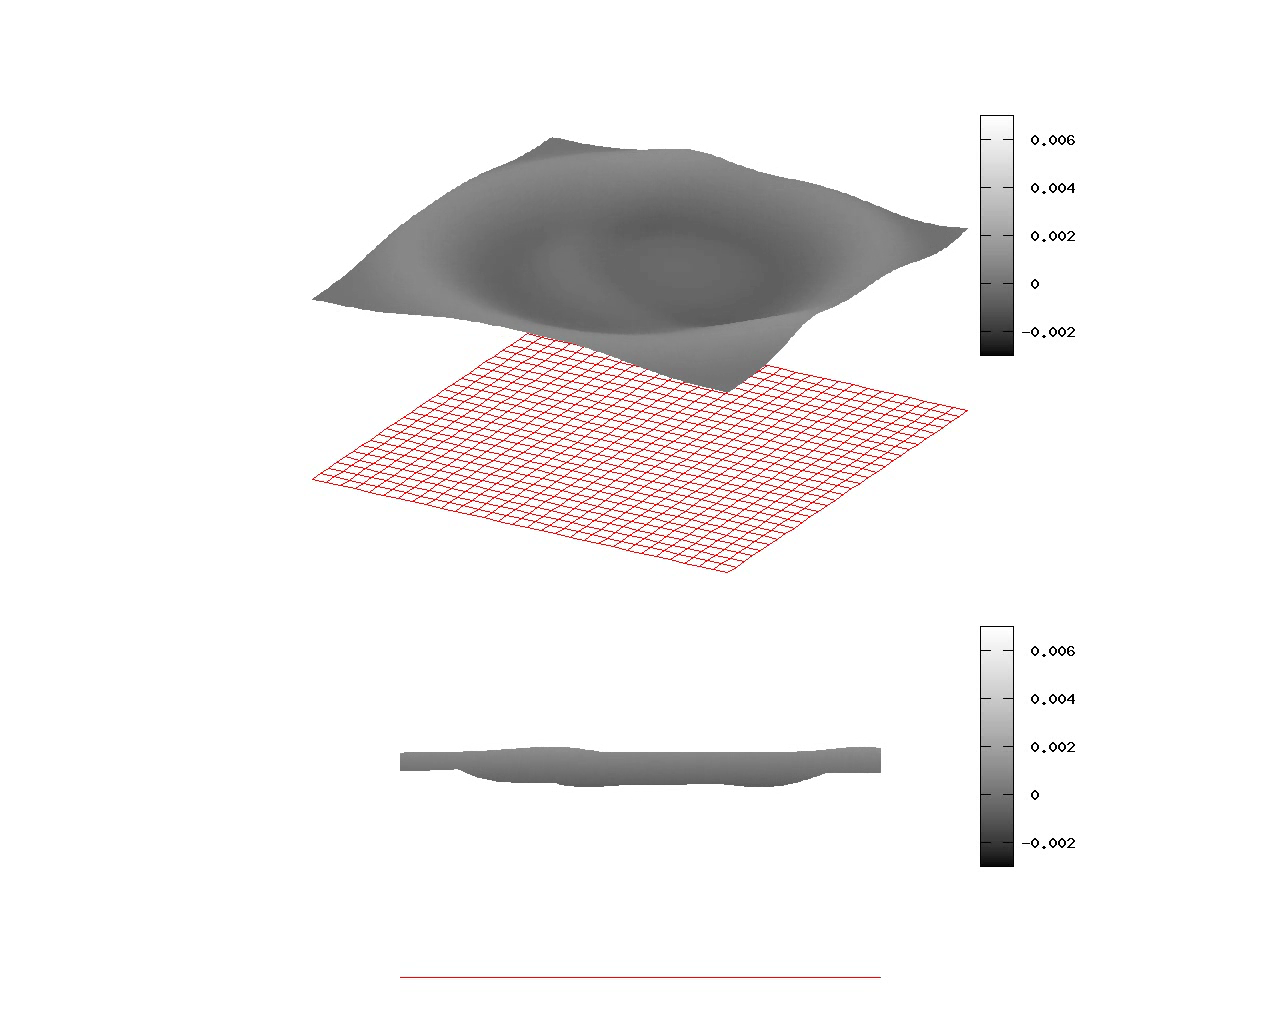
\includegraphics[width=8cm]{complex_drop3.png}
    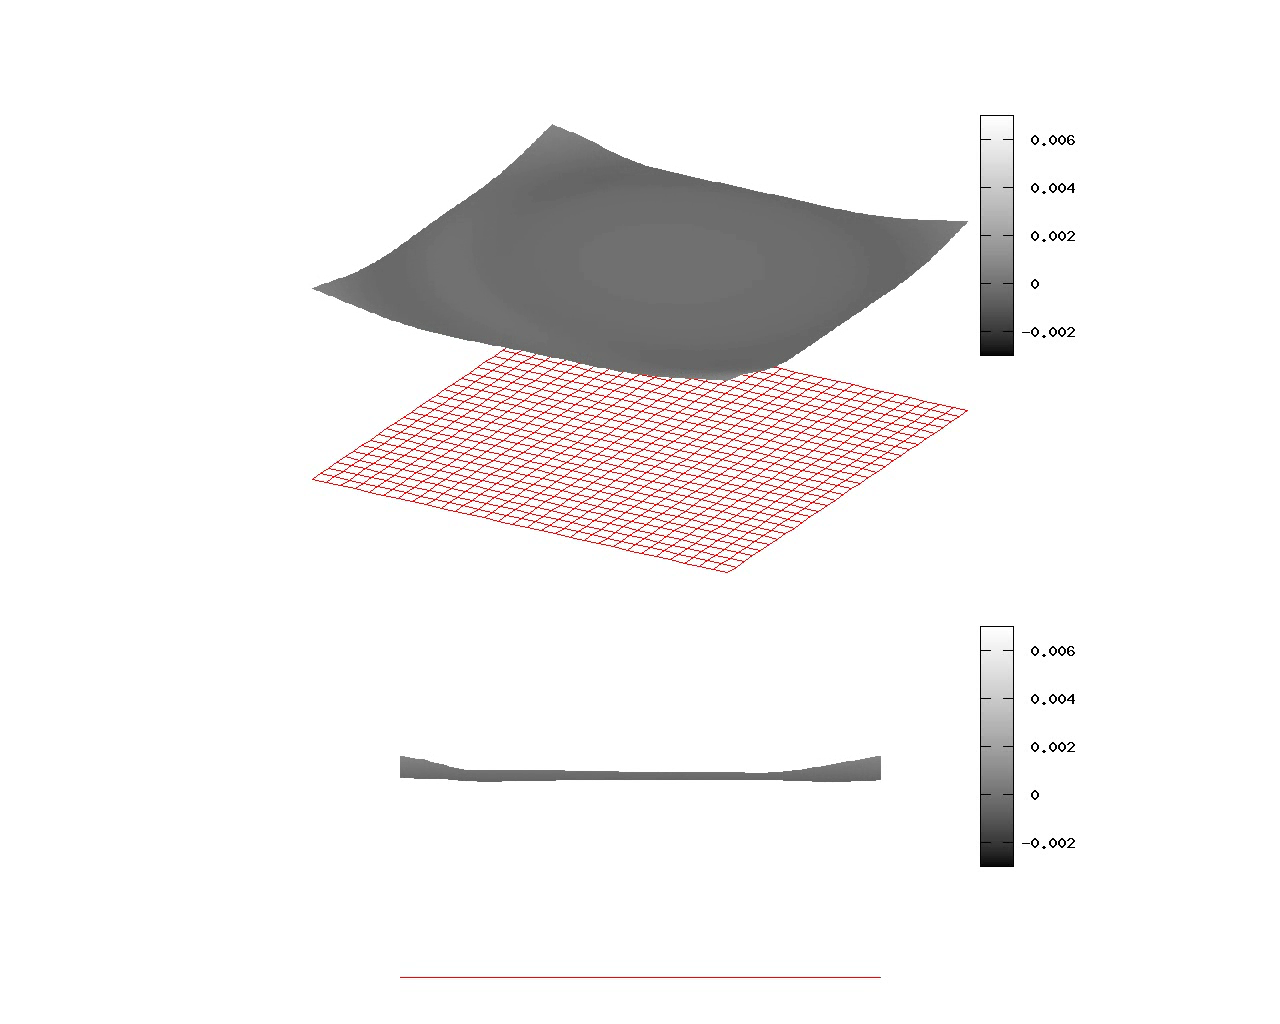
\includegraphics[width=8cm]{complex_drop4.png}
    \caption{Результат расчета для нелинейной системы($F_{nonlin}\neq 0$) со сложной начальной формой на нулевом, 80, 180 и 280 шаге}
    \label{fig:ComplexDrop}
\end{figure}

\newpage
Рассмотрим задачу о движении начальной волны следующего вида:

$u_0=0\;v_0=0\;\eta_0=4 \cdot 10^{-3}e^{-300 ((x-0.3)^2)}+4 \cdot 10^{-3}e^{(-300 ((x-0.7)^2+(y-0.7)^2))}$

в единичном квадрате глубиной $H(x,y)=10^{-2}$.

\begin{table}[H]
    \label{tab:FirstResult}
    \caption{Параметры для расчета со сложной формой поверхности}
    \begin{center}
	\begin{tabular}{|c|c|c|}
	    \hline
	    Размер области & $1\times1$\\
	    \hline
	    Количество шагов & $300$\\
	    \hline
	    Шаг по времени & $0.01$\\
	    \hline
	    Шаг сетки & $0.01$\\
	    \hline
	    Точность метода & $10^{-7}$\\
	    \hline
	    Форма дна & $H(x,y)=0.01\; B(x,y,t)=0$\\
	    \hline
	\end{tabular}
    \end{center}
\end{table}

На рис.\ref{fig:ComplexDrop2} представлена динамика выхода волны из области решения.

Как видно из представленных расчетов, предлагаемый подход к решению задачи (\ref{eq:MainVectorForm})-(\ref{eq:BoundaryCondition}) позволяет находить в ней решение без отражений или искажений. Волна, движущаяся в расчетной области, проходит через искусственные границы корректно.

\newpage
\begin{figure}[htp]
    \centering
    \vspace{12em}
    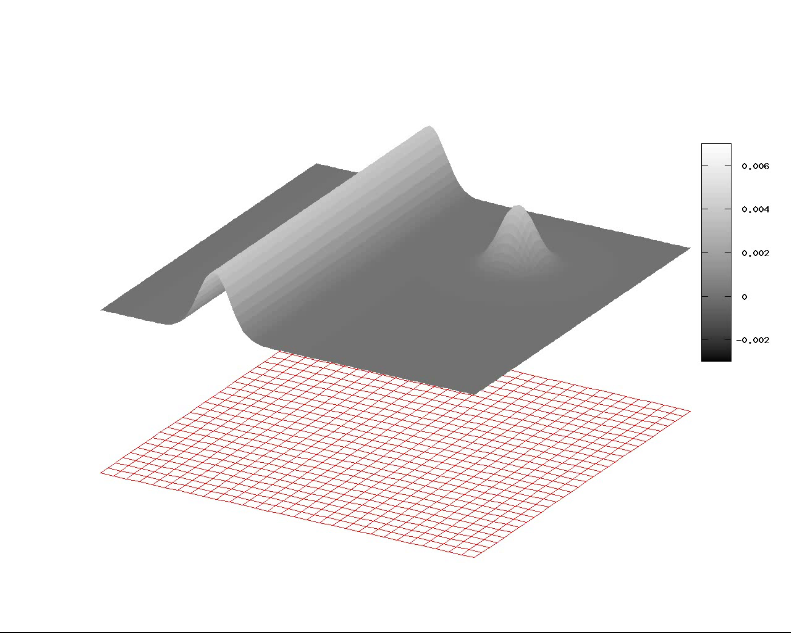
\includegraphics[width=8cm,trim=0 4mm 0 0,clip]{out_nonlin_complex_start21.png}
    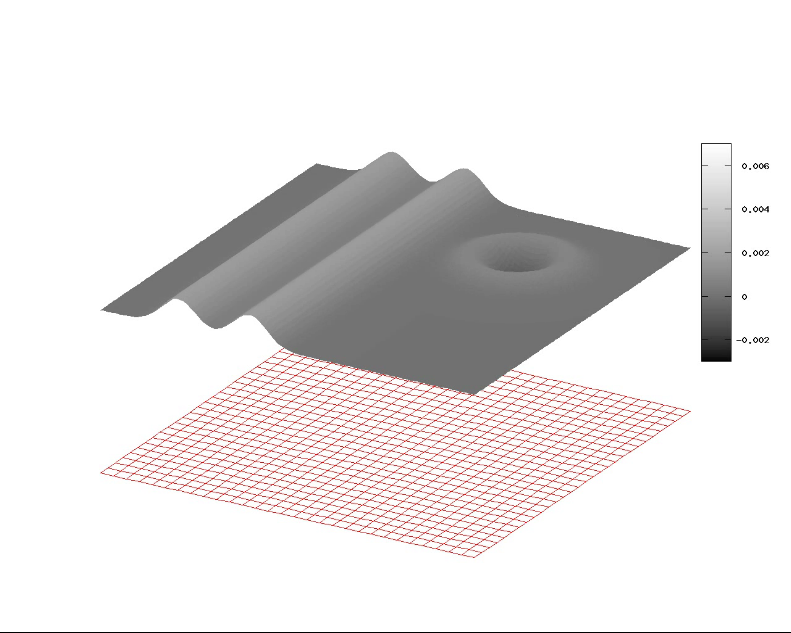
\includegraphics[width=8cm,trim=0 4mm 0 0,clip]{out_nonlin_complex_start22.png}
    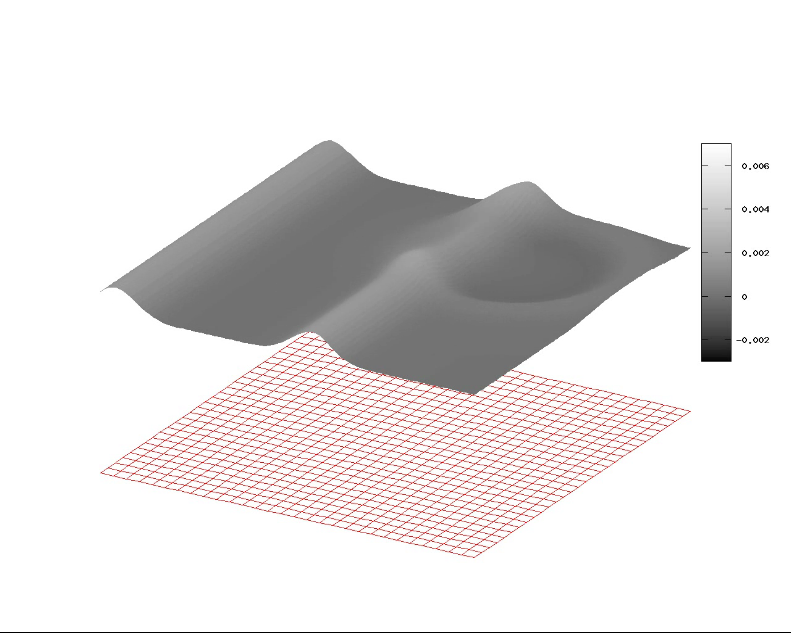
\includegraphics[width=8cm,trim=0 4mm 0 0,clip]{out_nonlin_complex_start23.png}
    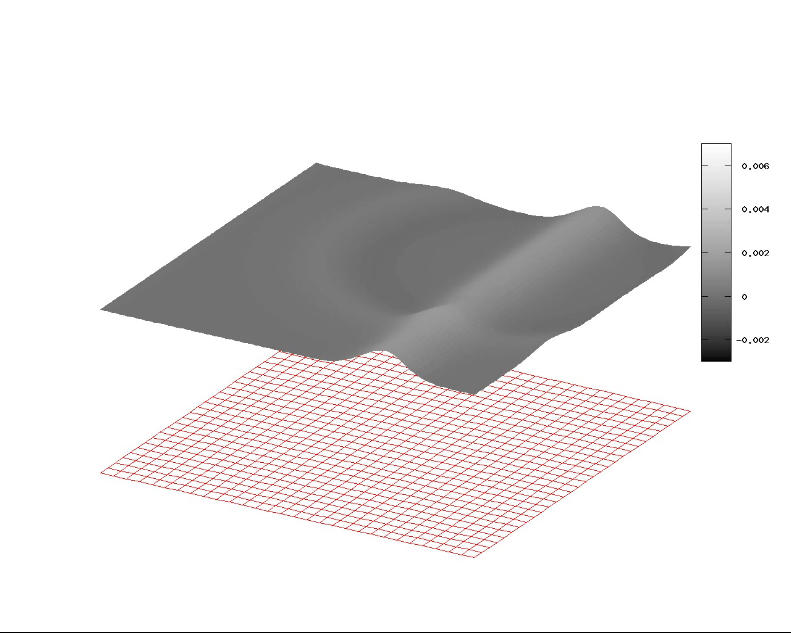
\includegraphics[width=8cm,trim=0 4mm 0 0,clip]{out_nonlin_complex_start24.png}
    \caption{Результат расчета для нелинейной системы($F_{nonlin}\neq 0$) со сложной начальной формой (длинная волна и <<капля>>) на нулевом, 80, 180 и 280 шаге}
    \label{fig:ComplexDrop2}
\end{figure}

\newpage
\addtocounter{section}{1}
\setcounter{equation}{0}
\setcounter{subsection}{0}
\section*{Расчет движения над сложным дном} 
\addtocontents{toc}{\contentsline{section}{\protect\numberline{\S\;\thesection.}\vspace{10pt}Расчет движения над сложным дном}{\thepage}}

Рассмотрим задачу о движении начальной волны следующего вида:

$u_0=0\;v_0=0\;\eta_0=4 \cdot 10^{-3}e^{(-100 (x-0.7)^2)}$

в единичном квадрате глубиной $H(x,y)=10^{-2}$.

\begin{table}[H]
    \label{tab:FirstResult}
    \caption{Параметры для расчета с коническим выступом}
    \begin{center}
	\begin{tabular}{|c|c|c|}
	    \hline
	    Размер области & $1\times1$\\
	    \hline
	    Количество шагов & $1200$\\
	    \hline
	    Шаг по времени & $0.001$\\
	    \hline
	    Шаг сетки & $0.01$\\
	    \hline
	    Точность метода & $10^{-6}$\\
	    \hline
	    Форма дна & $H(x,y)=0.01, \sqrt{(x-5)^2+(y-0.5)^2}>0.05$\\ 
	    & $H(x,y)=0.005, \sqrt{(x-5)^2+(y-0.5)^2}<0.05$\\
	    & $B(x,y,t)=0$\\
	    \hline
	\end{tabular}
    \end{center}
\end{table}

На рис.\ref{fig:CylinderBottom} представлена динамика выхода волны из области решения в двух проекциях для каждого шага.

На рис.\ref{fig:CylinderBottomMap} представлен тот же расчет в проекции свеху.

Видно, что волна, наталкиваясь на препятствие, замедляется в центре, откуда затем по поверхности начинают распространяться колебания.

\newpage
\begin{figure}[htp]
    \centering
    \vspace{12em}
    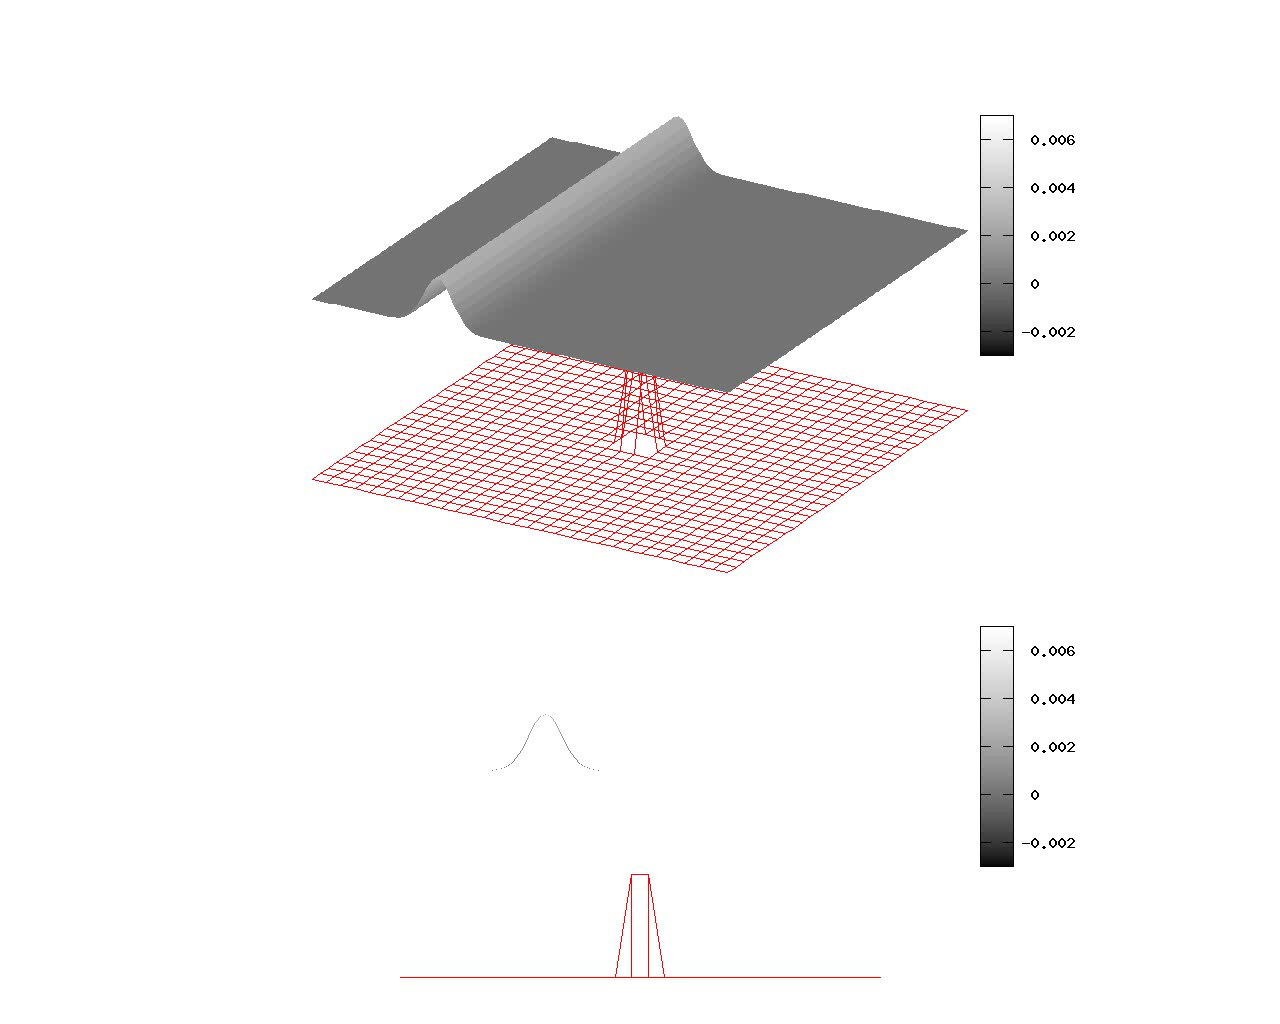
\includegraphics[width=8cm]{cylinder_bottom1.png}
    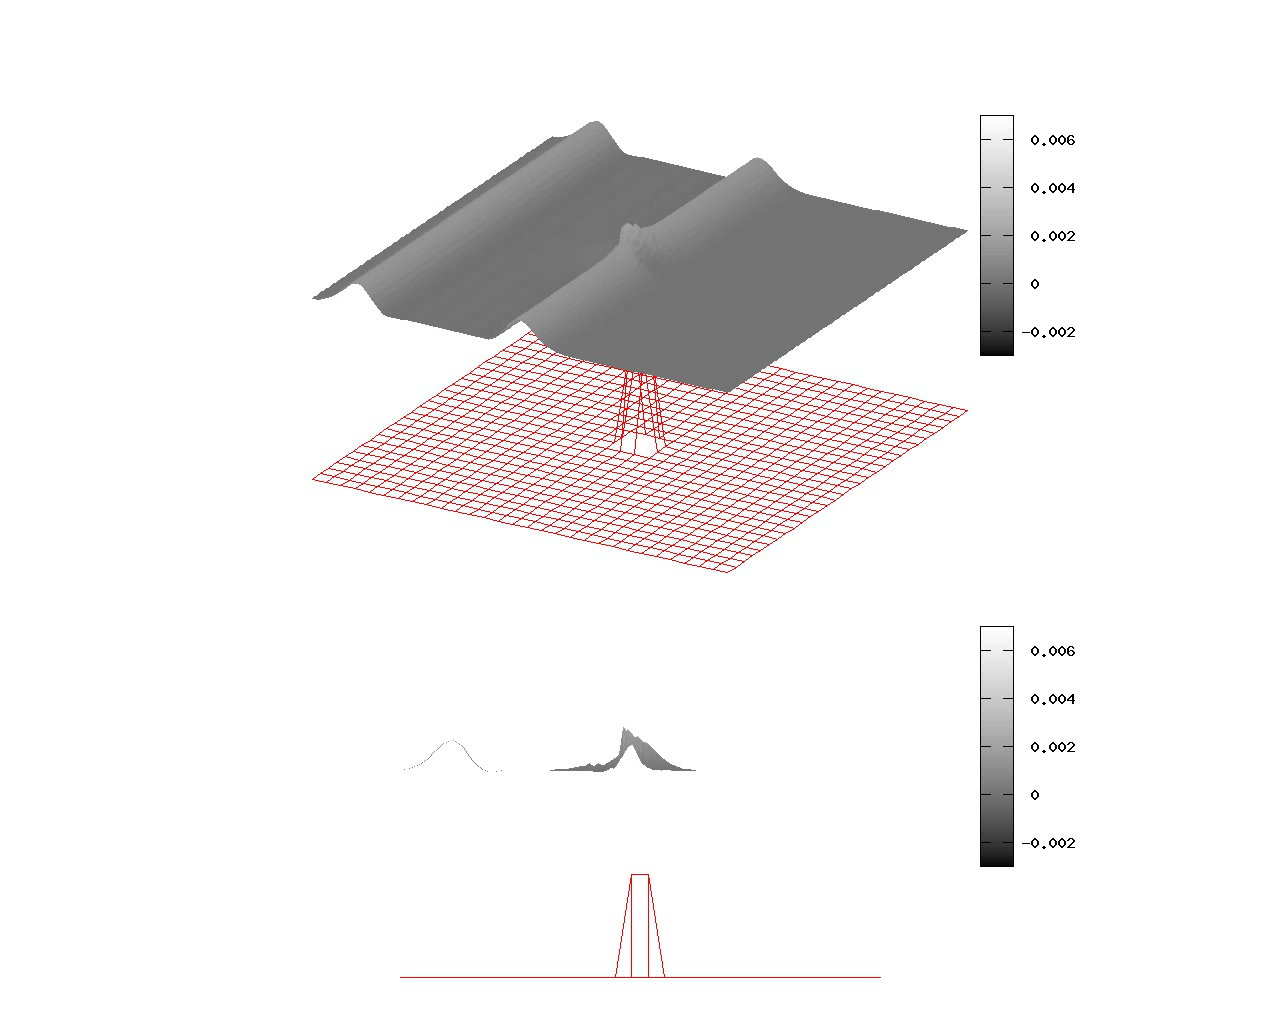
\includegraphics[width=8cm]{cylinder_bottom2.png}
    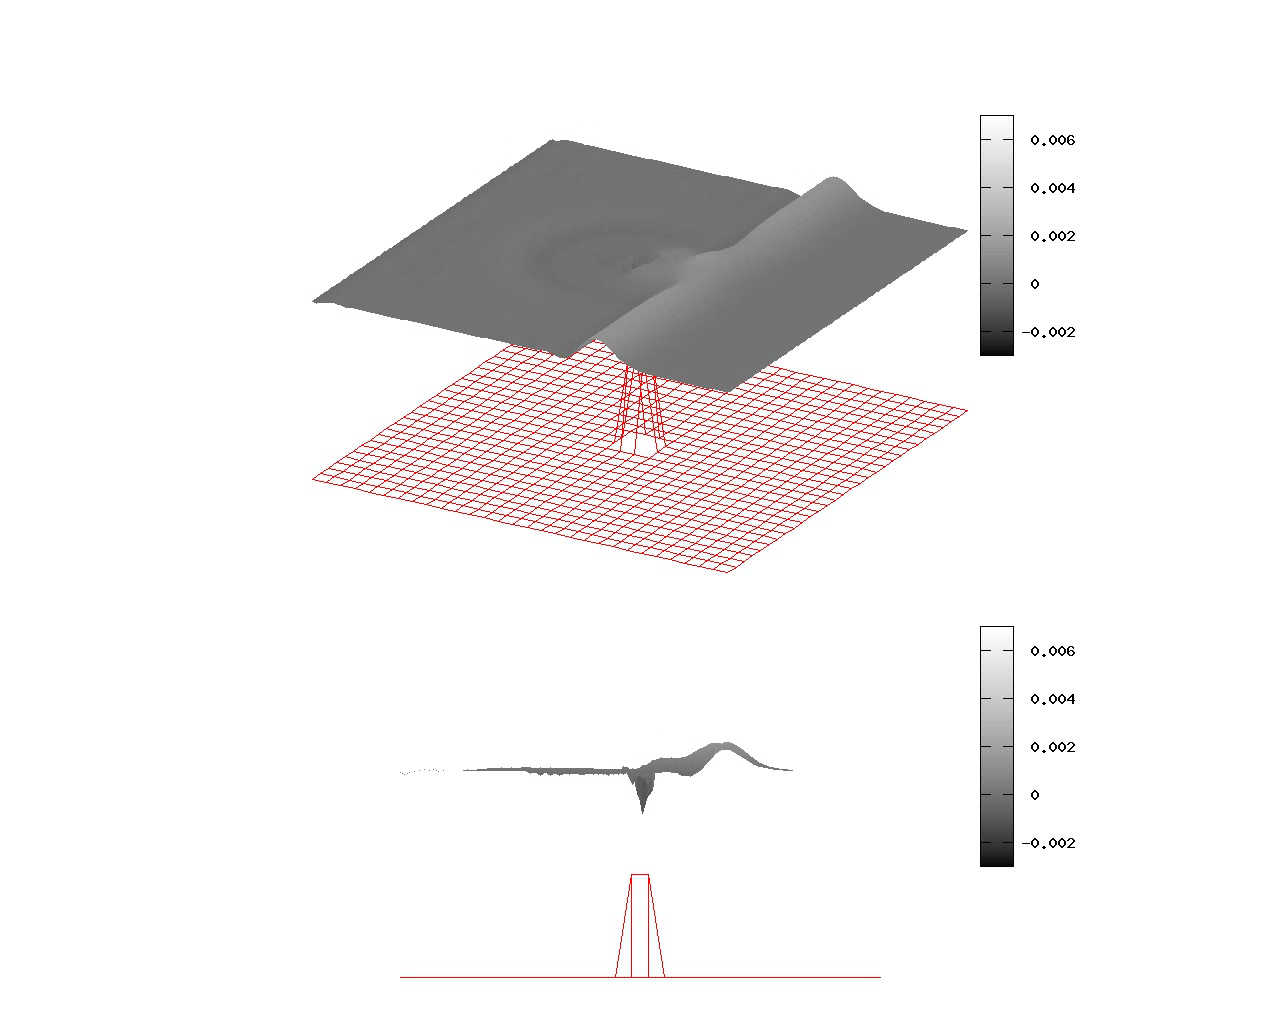
\includegraphics[width=8cm]{cylinder_bottom3.png}
    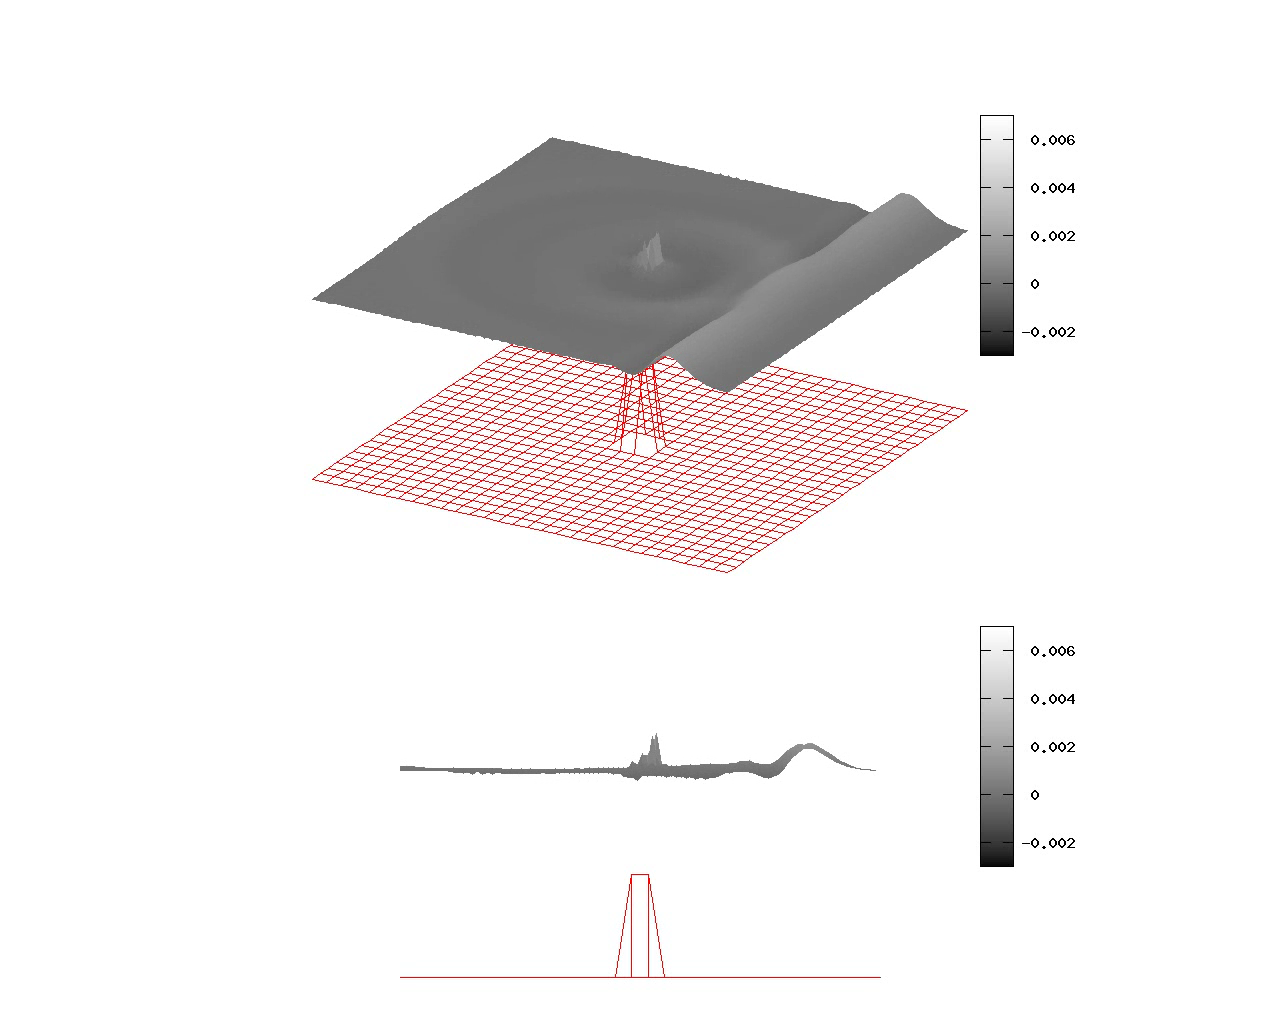
\includegraphics[width=8cm]{cylinder_bottom4.png}
    \caption{Результат расчета для нелинейной системы($F_{nonlin}\neq 0$) с коническим выступом дна на нулевом, 400, 800 и 1200 шаге}
    \label{fig:CylinderBottom}
\end{figure}

\newpage
\begin{figure}[htp]
    \centering
    \vspace{12em}
    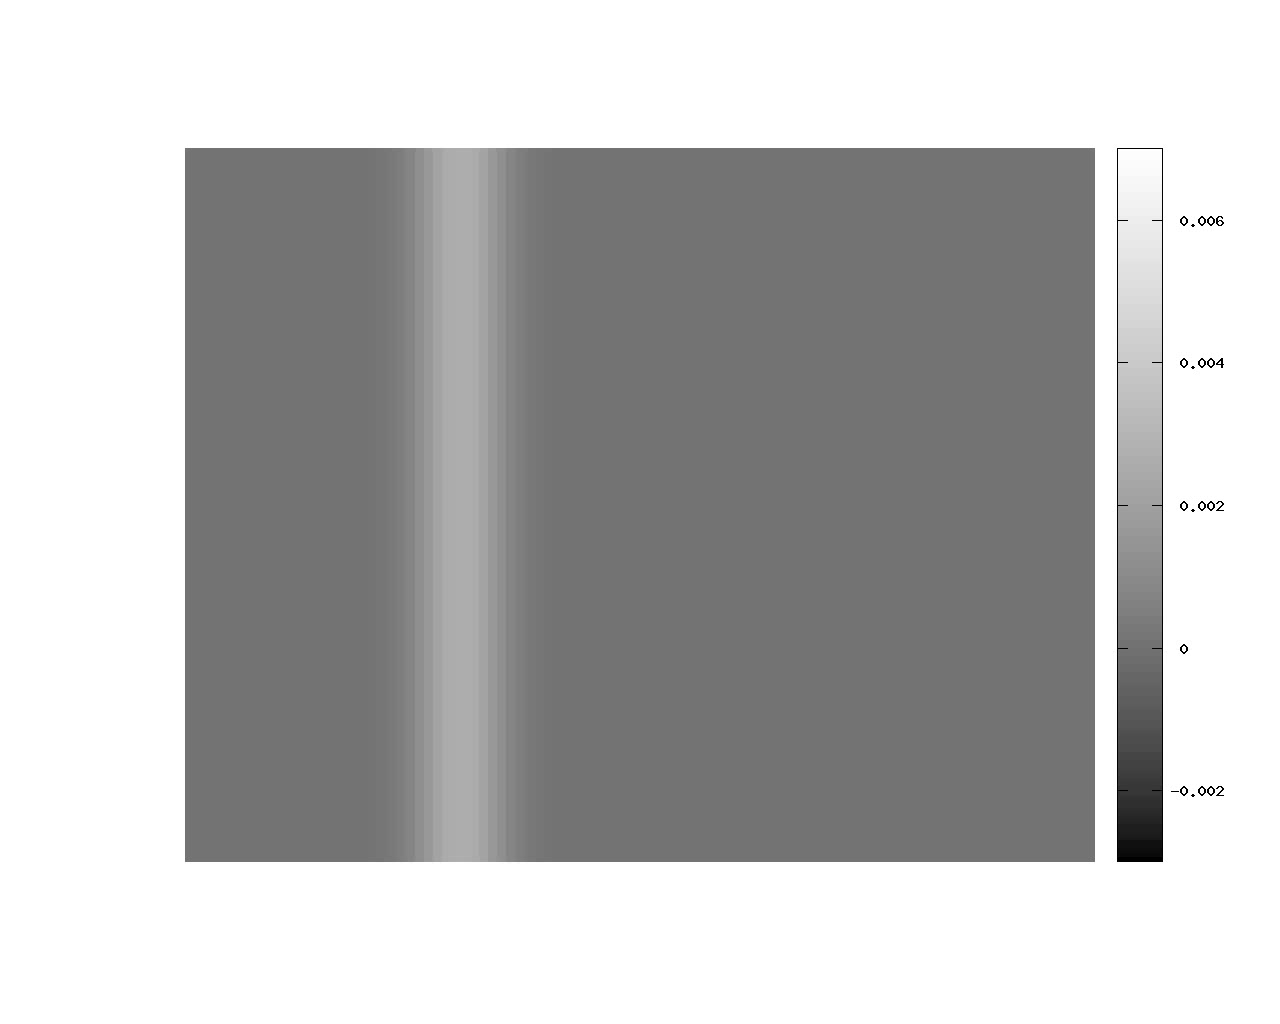
\includegraphics[width=8cm]{cylinder_bottom_map1.png}
    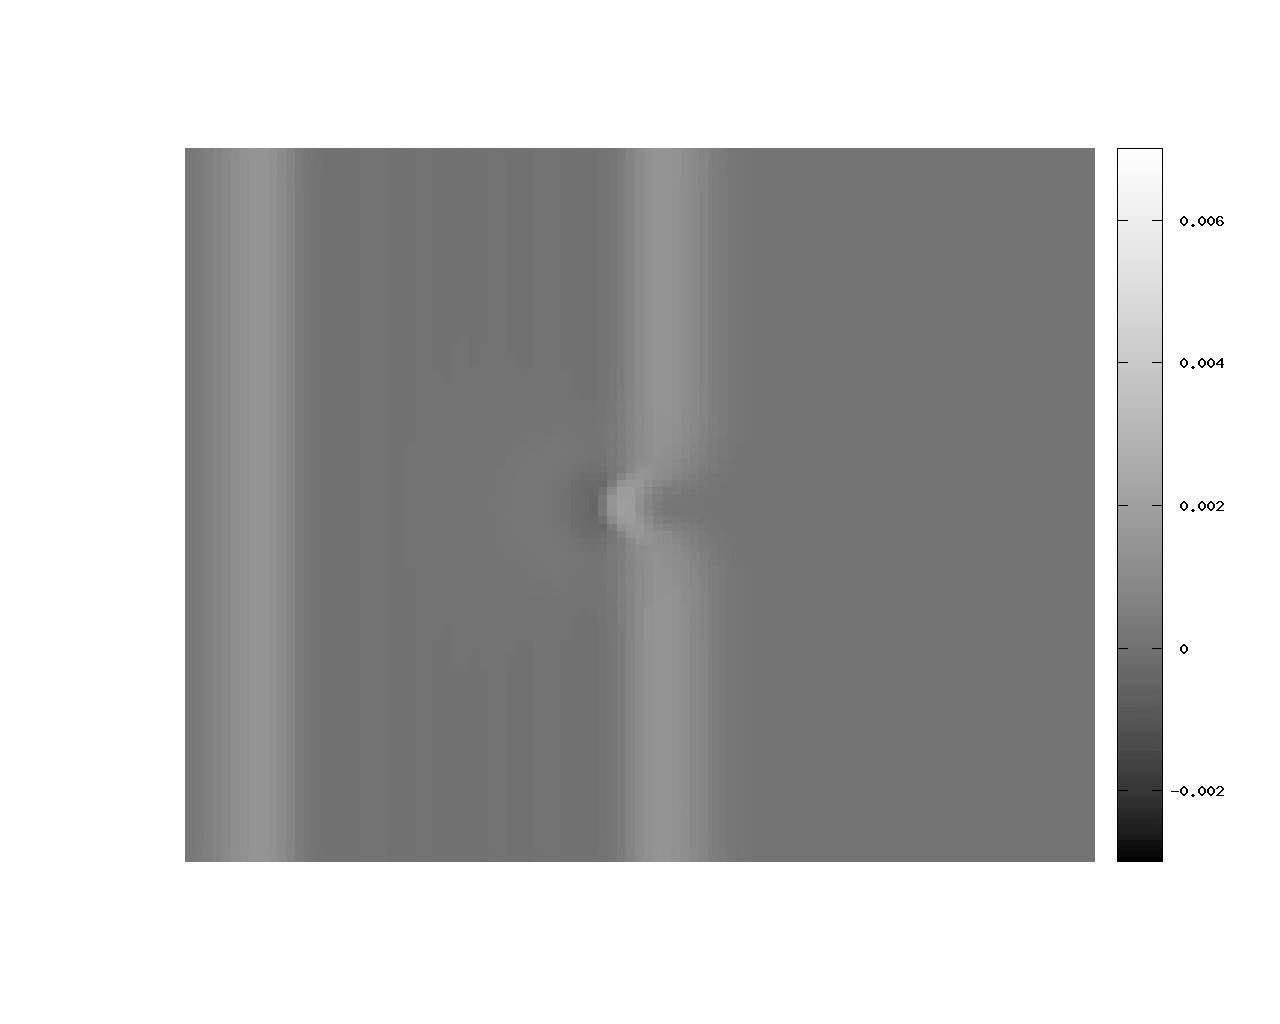
\includegraphics[width=8cm]{cylinder_bottom_map2.png}
    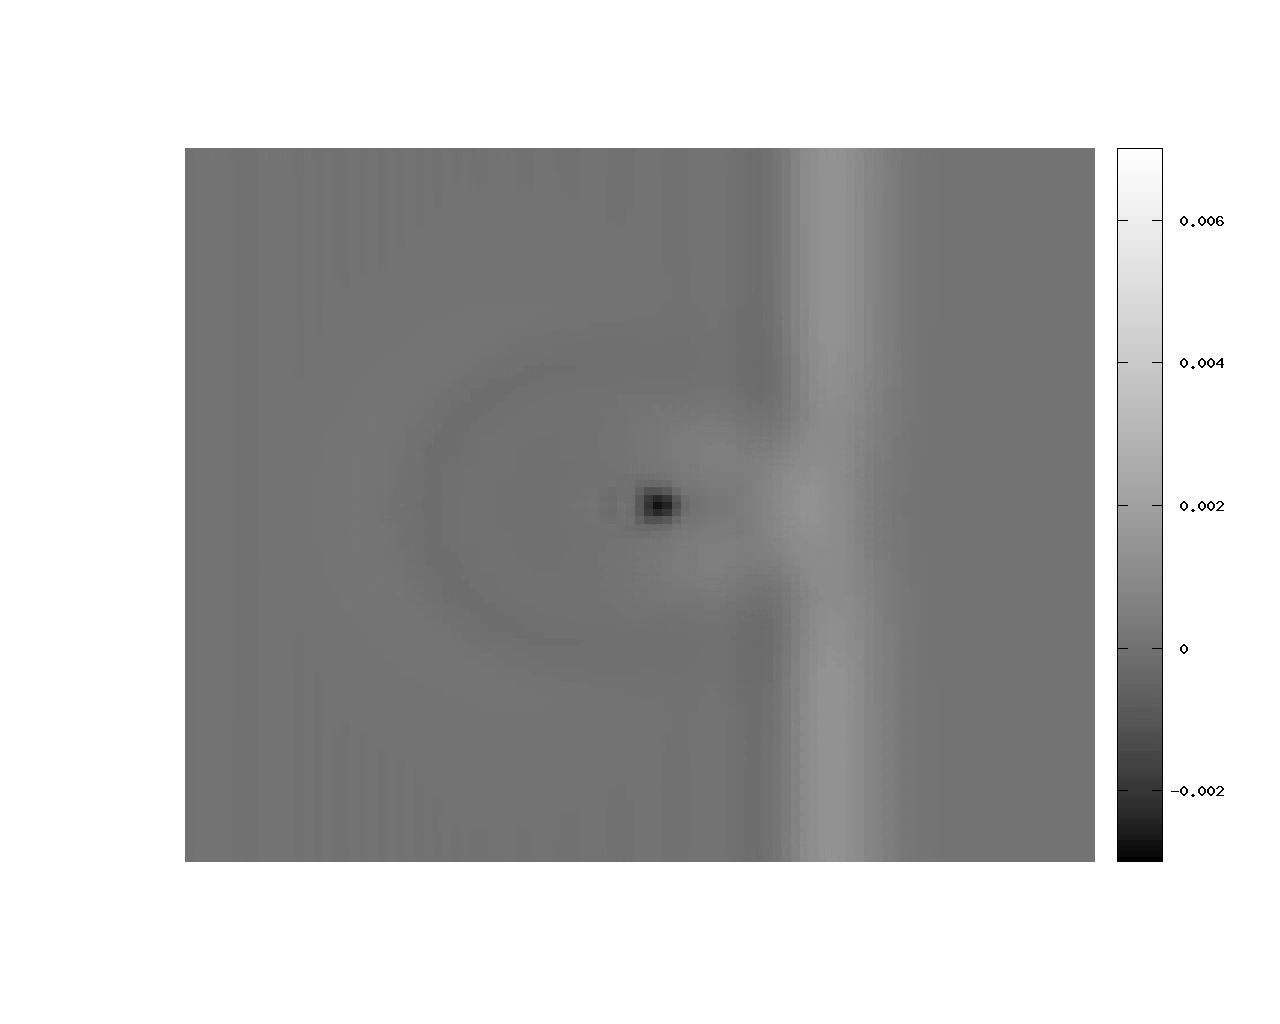
\includegraphics[width=8cm]{cylinder_bottom_map3.png}
    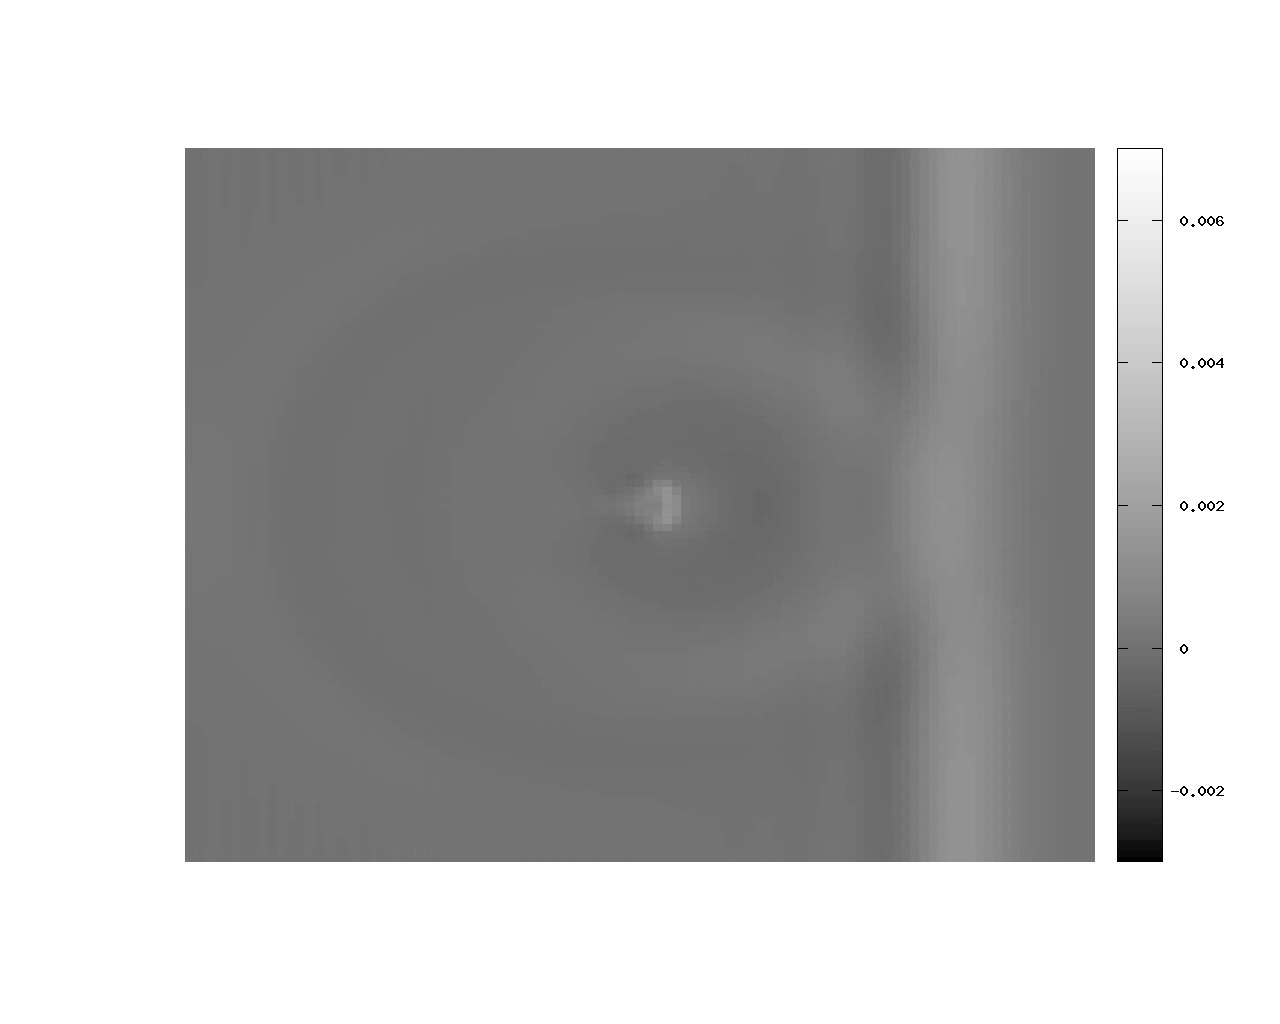
\includegraphics[width=8cm]{cylinder_bottom_map4.png}
    \caption{Результат расчета для нелинейной системы($F_{nonlin}\neq 0$) с коническим выступом дна на нулевом, 400, 800 и 1200 шаге (проекция сверху)}
    \label{fig:CylinderBottomMap}
\end{figure}

\newpage
Рассмотрим задачу о движении начальной волны следующего вида:

$u_0=0\;v_0=0\;\eta_0=7 \cdot 10^{-3}e^{(-100 (x-0.7)^2)}$

в единичном квадрате глубиной $H(x,y)=10^{-2}$.

\begin{table}[H]
    \label{tab:FirstResult}
    \caption{Параметры для расчета с экспоненциальным выступом}
    \begin{center}
	\begin{tabular}{|c|c|c|}
	    \hline
	    Размер области & $1\times1$\\
	    \hline
	    Количество шагов & $300$\\
	    \hline
	    Шаг по времени & $0.001$\\
	    \hline
	    Шаг сетки & $0.01$\\
	    \hline
	    Точность метода & $10^{-7}$\\
	    \hline
	    Форма дна & $H(x,y)=0.01-3 \cdot 10^{-3}e^{(-100 (x-0.7)^2)}$\\
	    & $B(x,y,t)=0$\\
	    \hline
	\end{tabular}
    \end{center}
\end{table}

На рис.\ref{fig:ExpBottom} представлена динамика выхода волны из области решения в двух проекциях для каждого шага.

Из расчетов, представленных в этом параграфе, видно, что предлагаемый подход к решению задачи (\ref{eq:MainVectorForm})-(\ref{eq:BoundaryCondition}) над неровным дном также позволяет находить решение без искажений или отражений. Волна, движущаяся в расчетной области, по-прежнему корректно проходит через искусственные границы, соответствующим образом изменяя свою форму над неровностями дна (например, замедляясь на подъемах).

\newpage
\begin{figure}[htp]
    \centering
    \vspace{12em}
    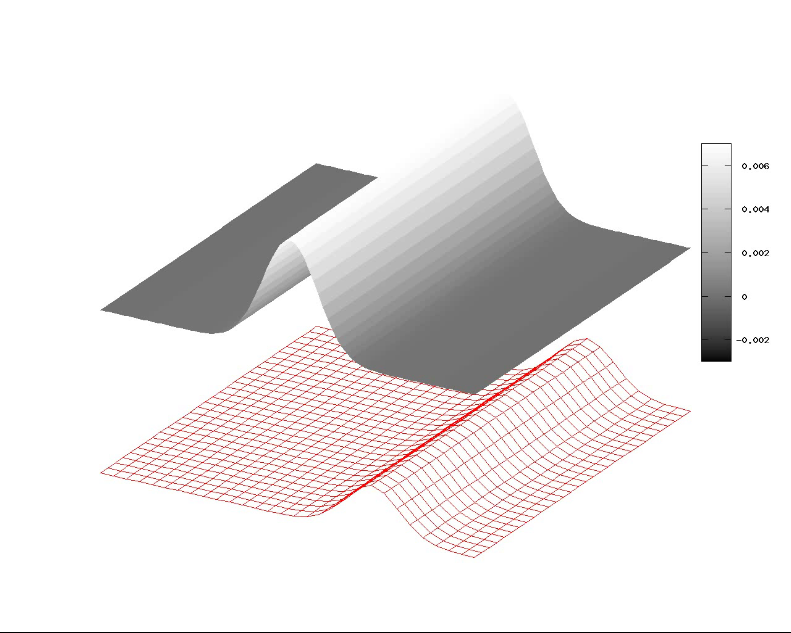
\includegraphics[width=8cm,trim=0 4mm 0 0,clip]{wave_on_exp1.png}
    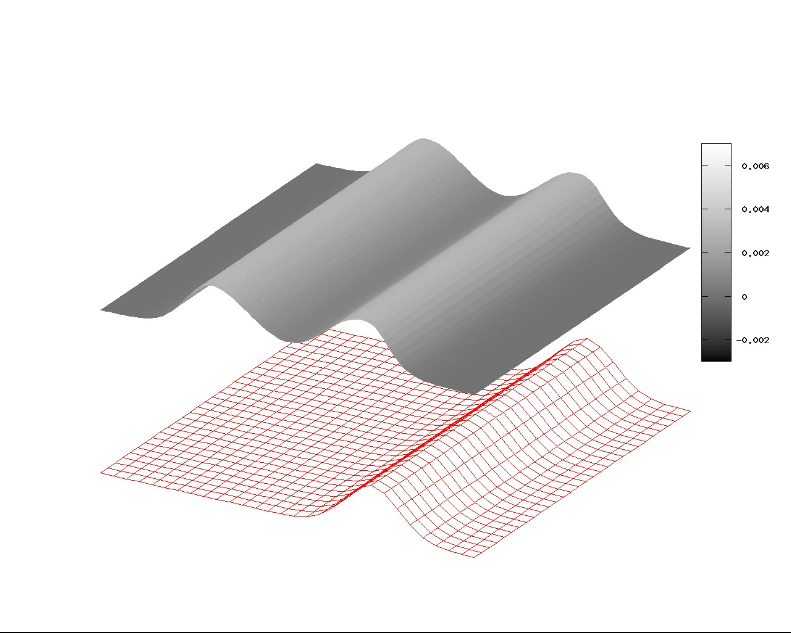
\includegraphics[width=8cm,trim=0 4mm 0 0,clip]{wave_on_exp2.png}
    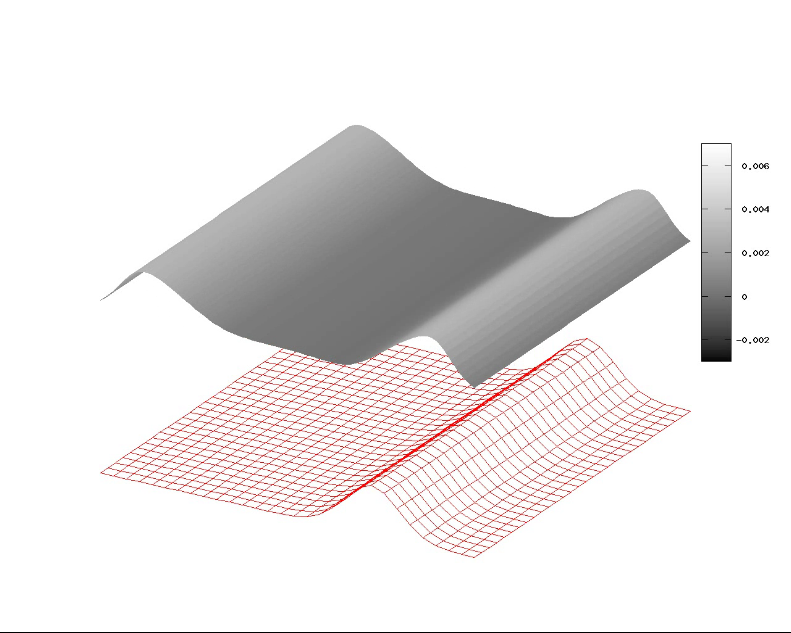
\includegraphics[width=8cm,trim=0 4mm 0 0,clip]{wave_on_exp3.png}
    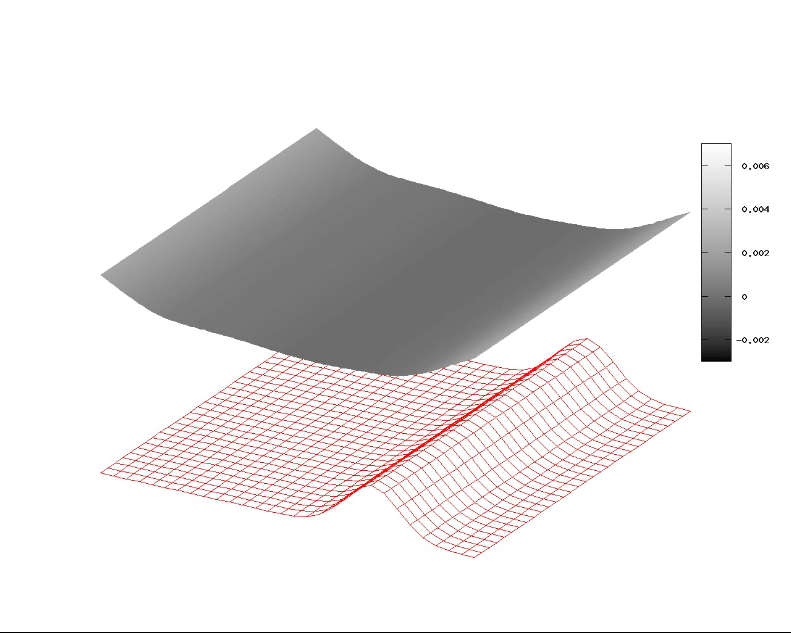
\includegraphics[width=8cm,trim=0 4mm 0 0,clip]{wave_on_exp4.png}
    \caption{Результат расчета для нелинейной системы($F_{nonlin}\neq 0$) с экспоненциальным выступом дна на нулевом, 80, 180 и 280 шаге}
    \label{fig:ExpBottom}
\end{figure}

\newpage
\addtocounter{section}{1}
\setcounter{equation}{0}
\setcounter{subsection}{0}
\section*{Сравнение линейных и нелинейных уравнений} 
\addtocontents{toc}{\contentsline{section}{\protect\numberline{\S\;\thesection.}\vspace{10pt}Сравнение линейных и нелинейных уравнений}{\thepage}}

Рассмотрим задачу о движении начальной волны следующего вида:

$u_0=0\;v_0=0\;\eta_0=7 \cdot 10^{-3}e^{(-100 (x-0.5)^2)}$

в единичном квадрате глубиной $H(x,y)=10^{-2}$.

\begin{table}[H]
    \label{tab:FirstResult}
    \caption{Параметры для расчетов со сравнением линейных и нелинейных уравнений}
    \begin{center}
	\begin{tabular}{|c|c|c|}
	    \hline
	    Размер области & $1\times1$\\
	    \hline
	    Количество шагов & $300$\\
	    \hline
	    Шаг по времени & $0.01$\\
	    \hline
	    Шаг сетки & $0.01$\\
	    \hline
	    Точность метода & $10^{-7}$\\
	    \hline
	    Форма дна & $H(x,y)=0.01\;B(x,y,t)=0$\\
	    \hline
	\end{tabular}
    \end{center}
\end{table}

На рис.\ref{fig:SimpleWaveLin} представлена динамика выхода волны из области решения в случае линейных уравнений.

На рис.\ref{fig:SimpleWaveNonLin} представлена динамика выхода волны из области решения в случае нелинейных уравнений.

На рис.\ref{fig:SimpleWaveDelta} представлена динамика разности этих расчетов.

Заметно, что расчет с нелинейными уравнениями отличается от аналогичного с линейными уравнениями. В линейном случае волна более симметрична относительно своей оси, в нелинейном - форма волны наклоняется в сторону движения.

\newpage
\begin{figure}[htp]
    \centering
    \vspace{12em}
    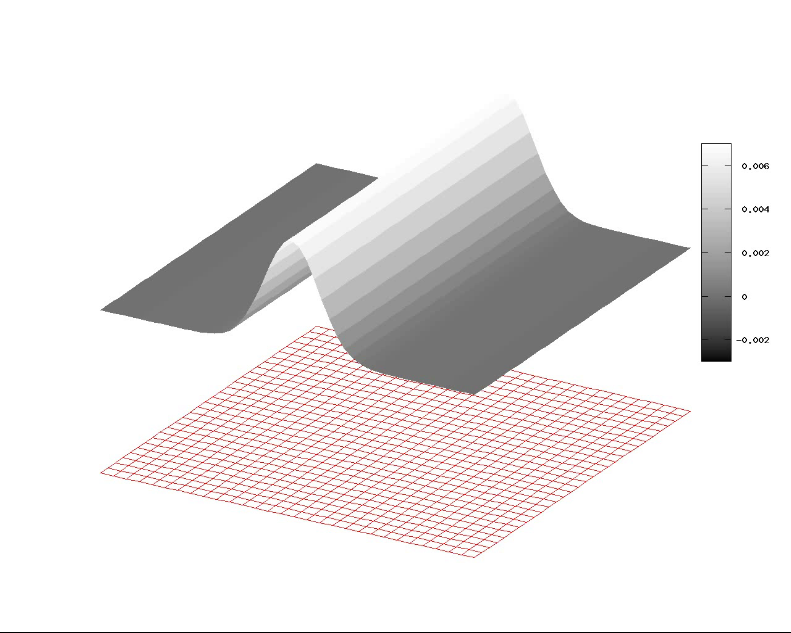
\includegraphics[width=8cm,trim=0 4mm 0 0,clip]{simple_wave_lin1.png}
    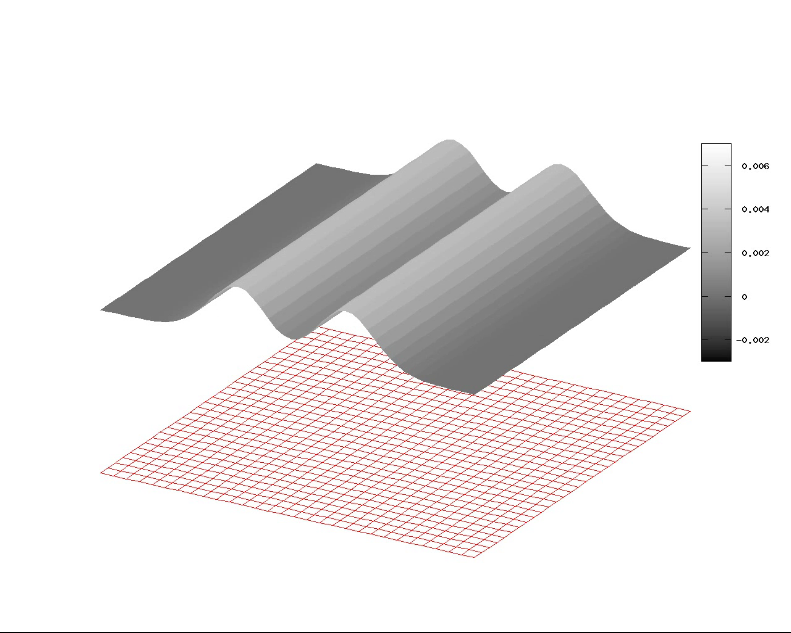
\includegraphics[width=8cm,trim=0 4mm 0 0,clip]{simple_wave_lin2.png}
    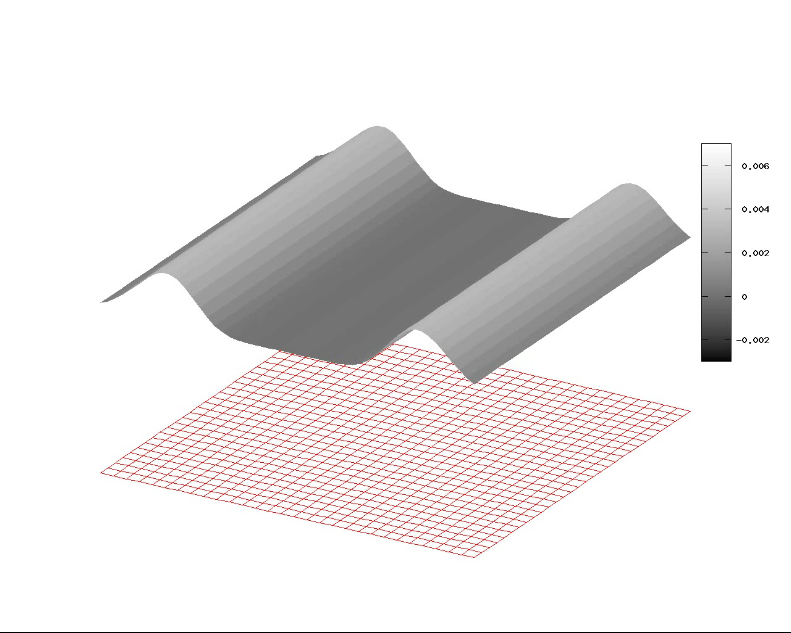
\includegraphics[width=8cm,trim=0 4mm 0 0,clip]{simple_wave_lin3.png}
    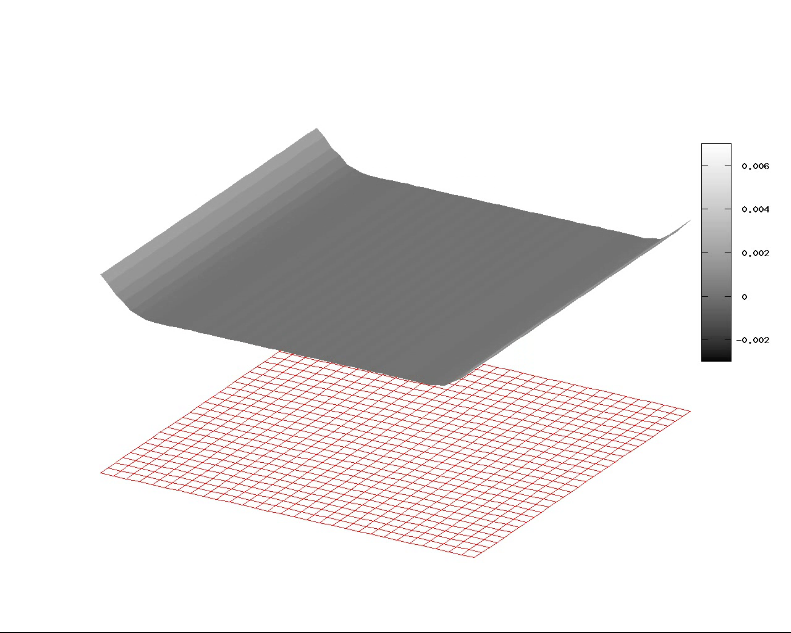
\includegraphics[width=8cm,trim=0 4mm 0 0,clip]{simple_wave_lin4.png}
    \caption{Результат расчета для линейной системы($F_{nonlin}=0$) с ровным дном на нулевом, 80, 180 и 280 шаге}
    \label{fig:SimpleWaveLin}
\end{figure}

\newpage
\begin{figure}[htp]
    \centering
    \vspace{12em}
    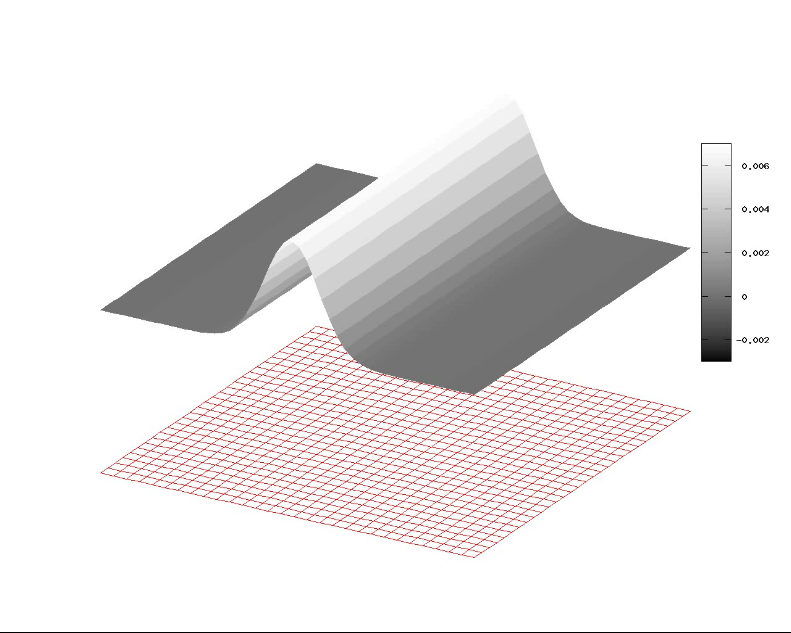
\includegraphics[width=8cm,trim=0 4mm 0 0,clip]{simple_wave_nonlin1.png}
    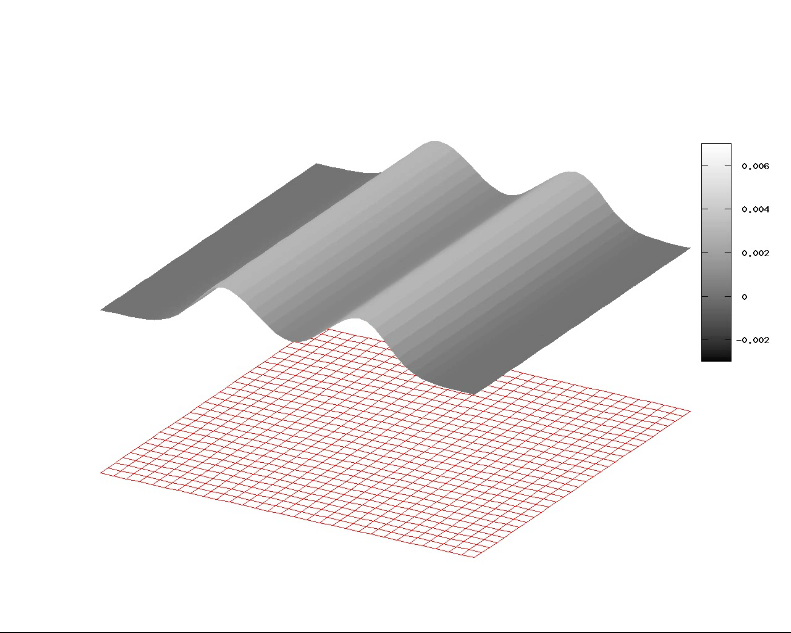
\includegraphics[width=8cm,trim=0 4mm 0 0,clip]{simple_wave_nonlin2.png}
    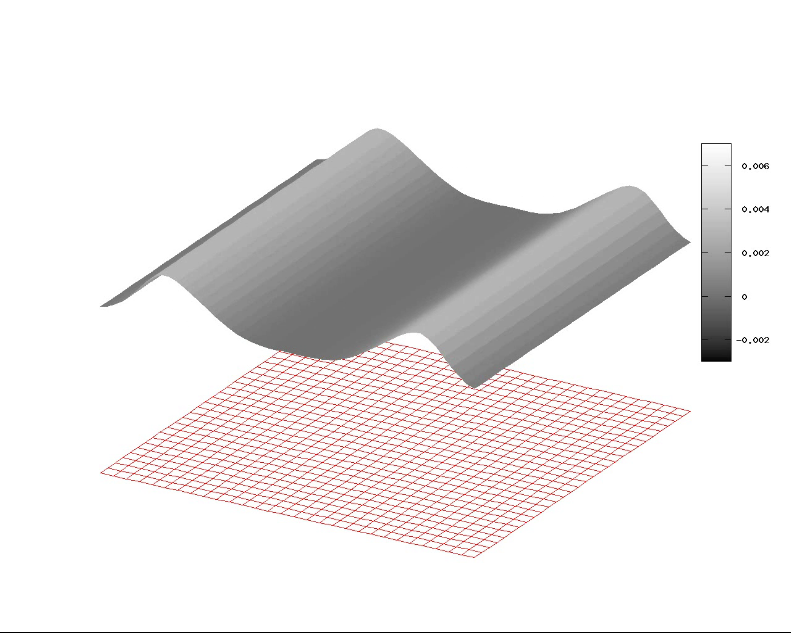
\includegraphics[width=8cm,trim=0 4mm 0 0,clip]{simple_wave_nonlin3.png}
    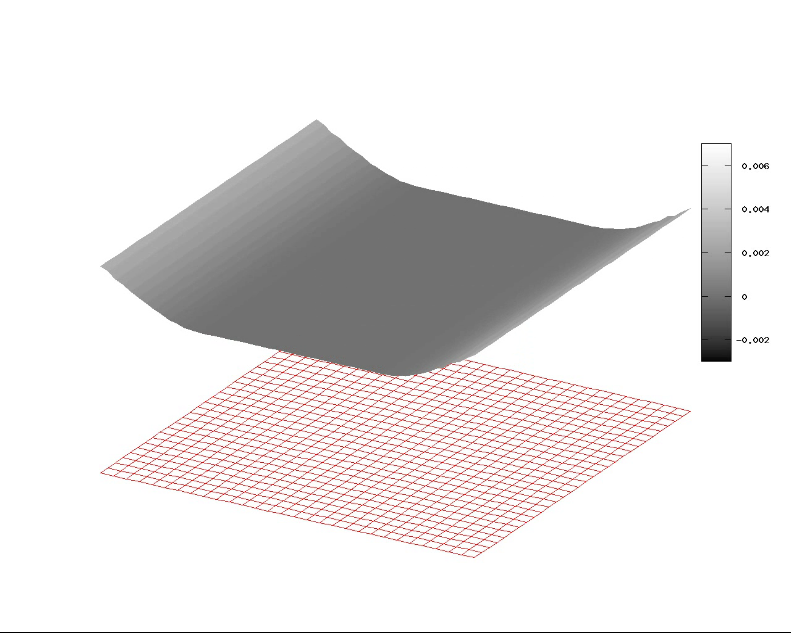
\includegraphics[width=8cm,trim=0 4mm 0 0,clip]{simple_wave_nonlin4.png}
    \caption{Результат расчета для нелинейной системы($F_{nonlin}\neq 0$) с ровным дном на нулевом, 80, 180 и 280 шаге}
    \label{fig:SimpleWaveNonLin}
\end{figure}

\newpage
\begin{figure}[htp]
    \centering
    \vspace{12em}
    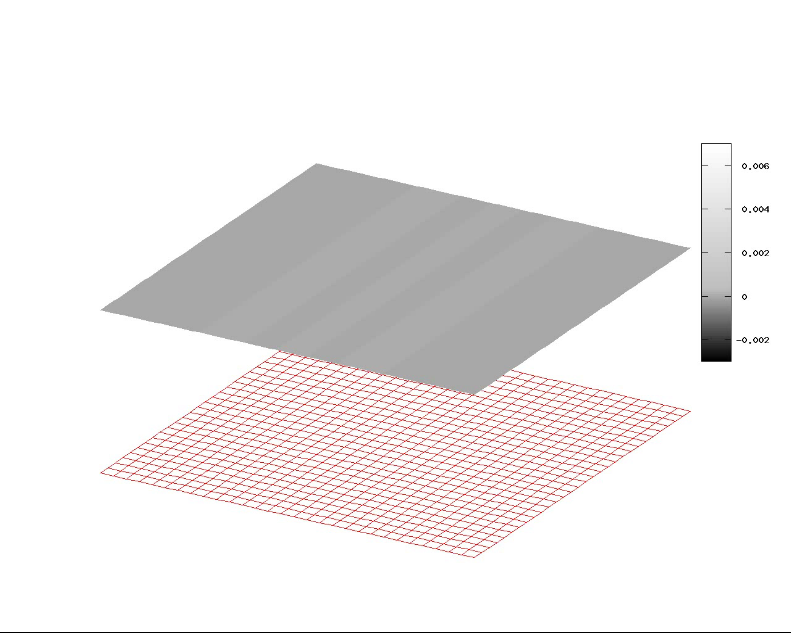
\includegraphics[width=8cm,trim=0 4mm 0 0,clip]{simple_wave_delta1.png}
    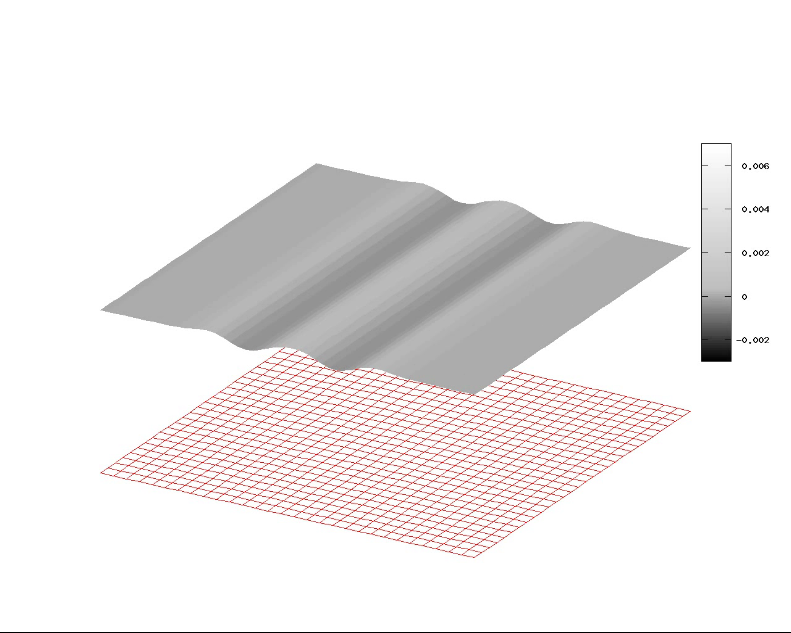
\includegraphics[width=8cm,trim=0 4mm 0 0,clip]{simple_wave_delta2.png}
    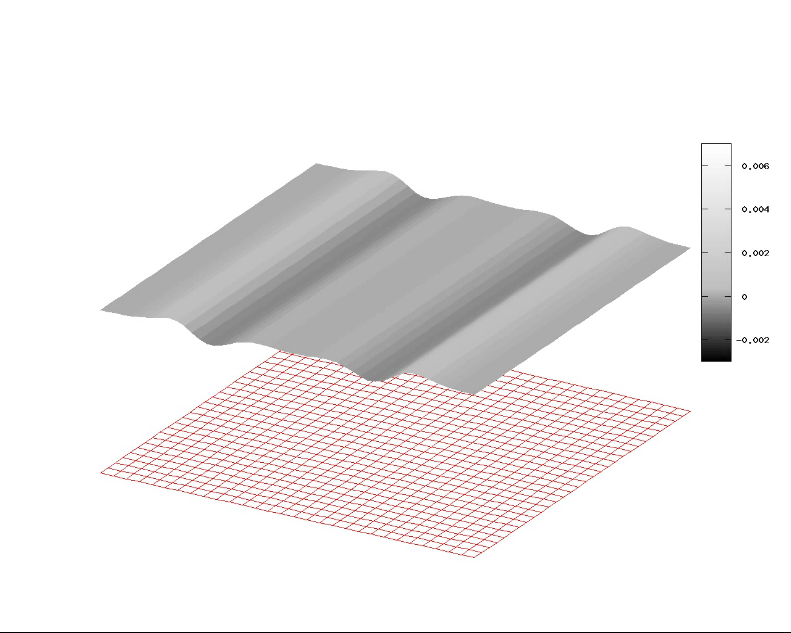
\includegraphics[width=8cm,trim=0 4mm 0 0,clip]{simple_wave_delta3.png}
    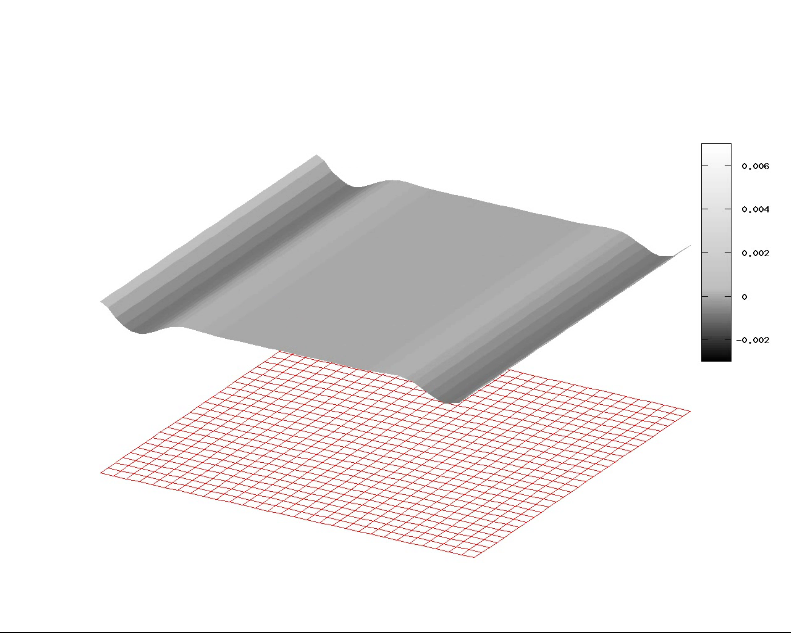
\includegraphics[width=8cm,trim=0 4mm 0 0,clip]{simple_wave_delta4.png}
    \caption{Динамика разности расчетов в линейном и нелинейном случае с ровным дном на нулевом, 80, 180 и 280 шаге}
    \label{fig:SimpleWaveDelta}
\end{figure}

\newpage
Рассмотрим задачу о движении начальной волны следующего вида:

$u_0=0\;v_0=0\;\eta_0=7 \cdot 10^{-3}e^{(-100 (x-0.5)^2)}$

в единичном квадрате глубиной $H(x,y)=10^{-2}$.

\begin{table}[H]
    \label{tab:FirstResult}
    \caption{Параметры для расчетов со сравнением линейных и нелинейных уравнений в случае дна с препятствием на границе}
    \begin{center}
	\begin{tabular}{|c|c|c|}
	    \hline
	    Размер области & $1\times1$\\
	    \hline
	    Количество шагов & $300$\\
	    \hline
	    Шаг по времени & $0.01$\\
	    \hline
	    Шаг сетки & $0.01$\\
	    \hline
	    Точность метода & $10^{-7}$\\
	    \hline
	    Форма дна & $H(x,y)=10^{-2}-3 \cdot 10^{-3}e^{(-100 (x-0.7)^2)}$\\
	    & $B(x,y,t)=0$\\
	    \hline
	\end{tabular}
    \end{center}
\end{table}

На рис.\ref{fig:ExpWaveLin} представлена динамика выхода волны из области решения в случае линейных уравнений.

На рис.\ref{fig:ExpWaveNonLin} представлена динамика выхода волны из области решения в случае нелинейных уравнений.

На рис.\ref{fig:ExpWaveDelta} представлена динамика разности этих расчетов в проекции сверху.

Исходя из представленных расчетов для линейных и нелинейных уравнений, можно отметить, что в нелинейном случае:
\begin{itemize}
    \item Волна со временем меняет свою форму. Она становится немного <<наклоненной>> вперед.
    \item После прохождения основной волны за ней тянется <<хвост>> из небольших колебаний.
    \item С течением времени данные эффекты проявляются более явно.
\end{itemize}

\newpage
\begin{figure}[htp]
    \centering
    \vspace{12em}
    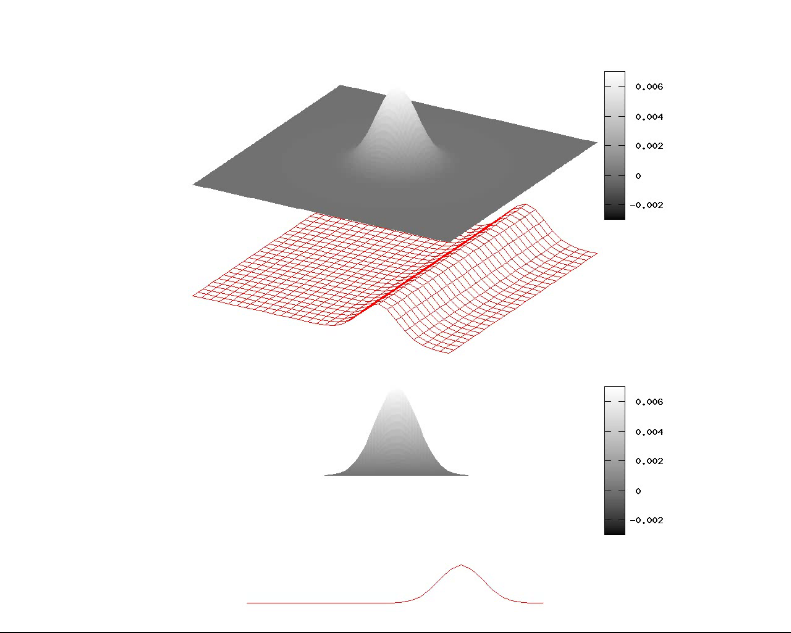
\includegraphics[width=8cm,trim=0 4mm 0 0,clip]{out_lin_drop_exp_bottom1.png}
    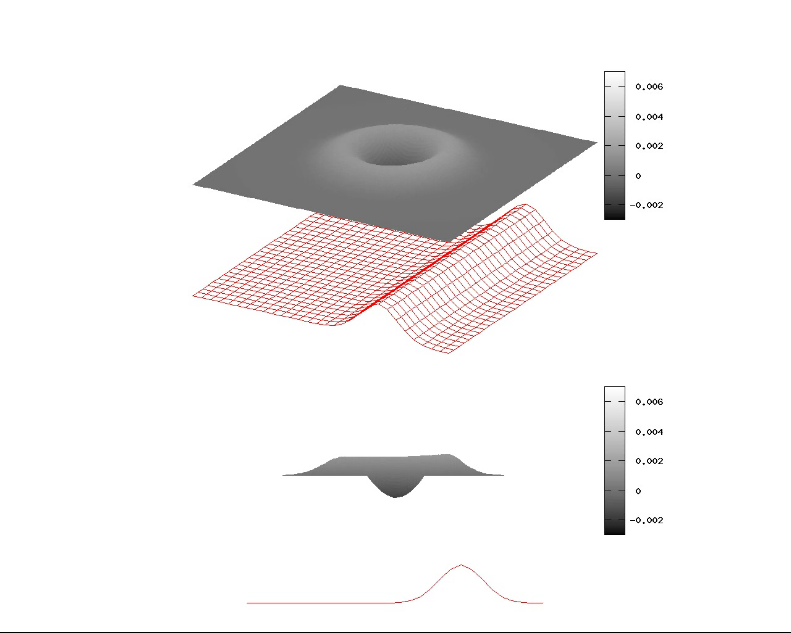
\includegraphics[width=8cm,trim=0 4mm 0 0,clip]{out_lin_drop_exp_bottom2.png}
    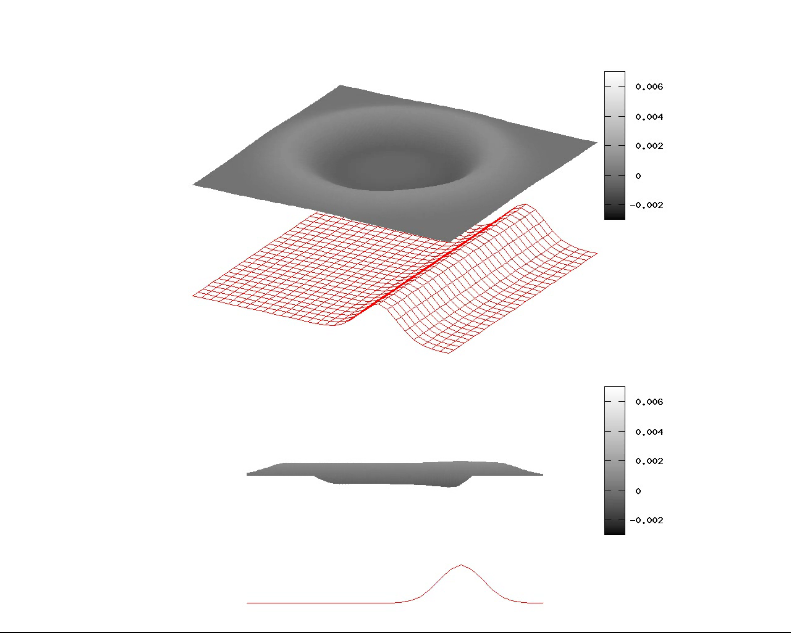
\includegraphics[width=8cm,trim=0 4mm 0 0,clip]{out_lin_drop_exp_bottom3.png}
    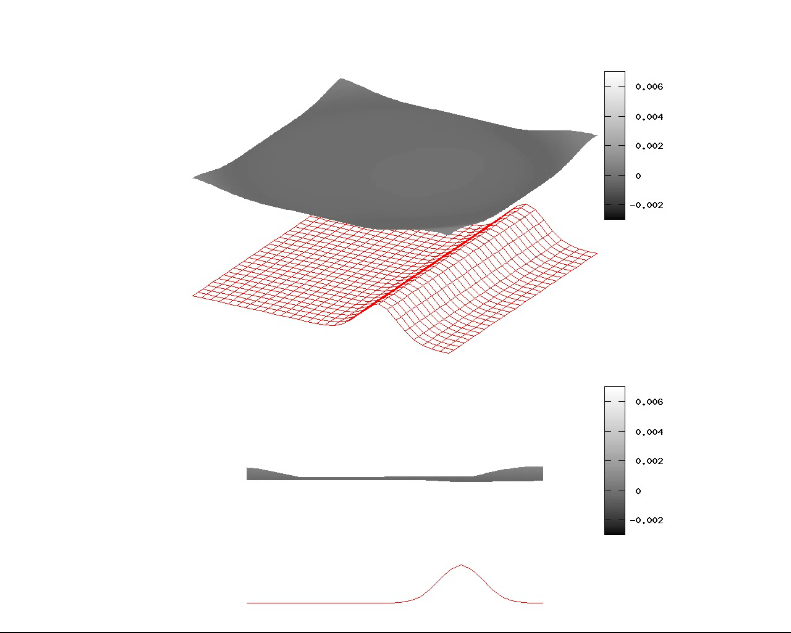
\includegraphics[width=8cm,trim=0 4mm 0 0,clip]{out_lin_drop_exp_bottom4.png}
    \caption{Результат расчета для линейной системы($F_{nonlin}=0$) с препятствием у границы на нулевом, 80, 200 и 380 шаге}
    \label{fig:ExpWaveLin}
\end{figure}

\newpage
\begin{figure}[htp]
    \centering
    \vspace{12em}
    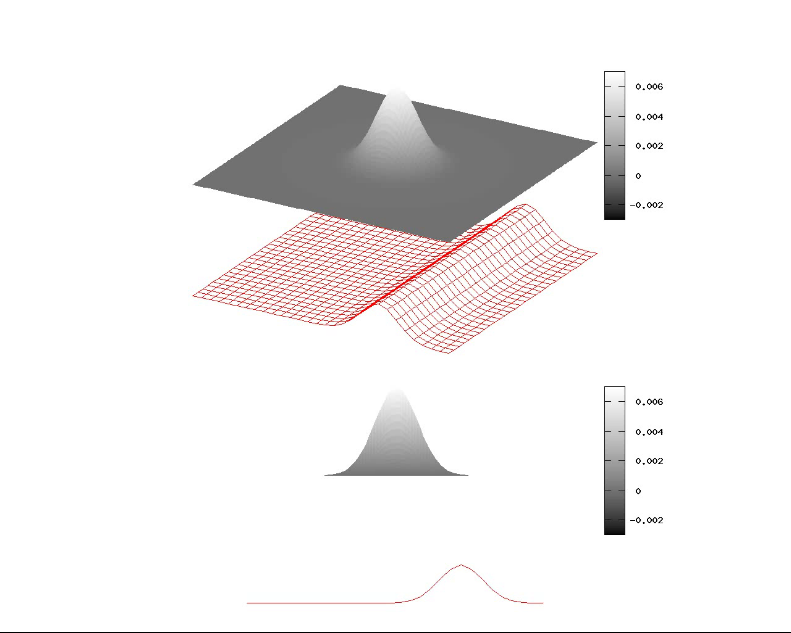
\includegraphics[width=8cm,trim=0 4mm 0 0,clip]{out_nonlin_drop_exp_bottom1.png}
    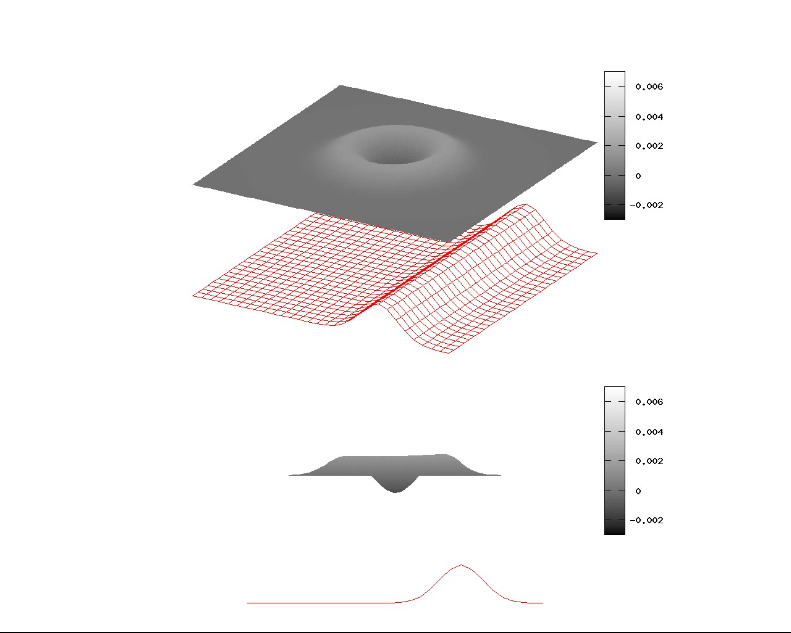
\includegraphics[width=8cm,trim=0 4mm 0 0,clip]{out_nonlin_drop_exp_bottom2.png}
    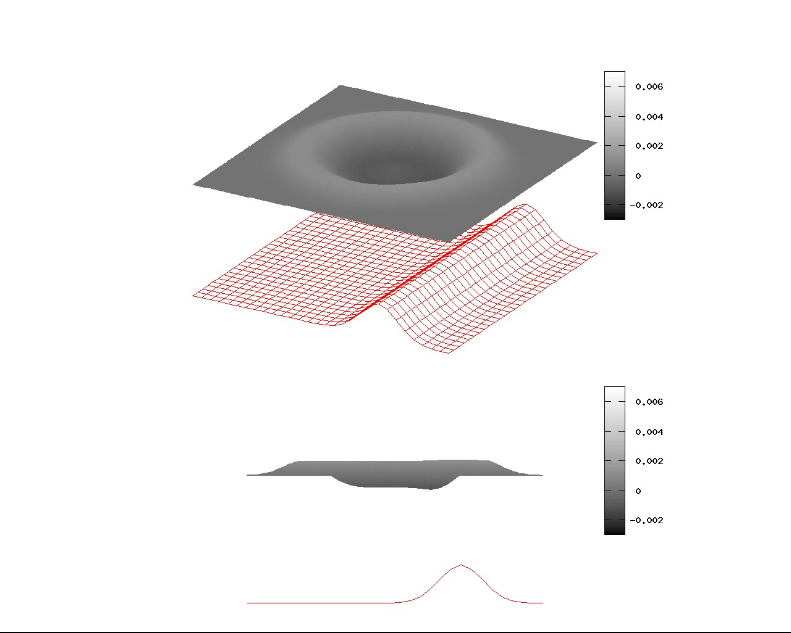
\includegraphics[width=8cm,trim=0 4mm 0 0,clip]{out_nonlin_drop_exp_bottom3.png}
    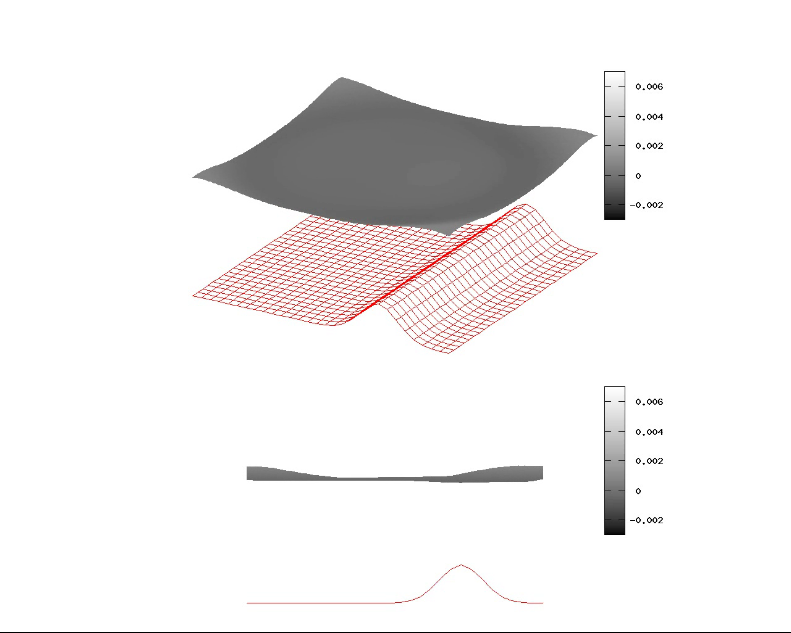
\includegraphics[width=8cm,trim=0 4mm 0 0,clip]{out_nonlin_drop_exp_bottom4.png}
    \caption{Результат расчета для нелинейной системы($F_{nonlin}\neq 0$) с препятствием у границы на нулевом, 80, 200 и 380 шаге}
    \label{fig:ExpWaveNonLin}
\end{figure}

\newpage
\begin{figure}[htp]
    \centering
    \vspace{12em}
    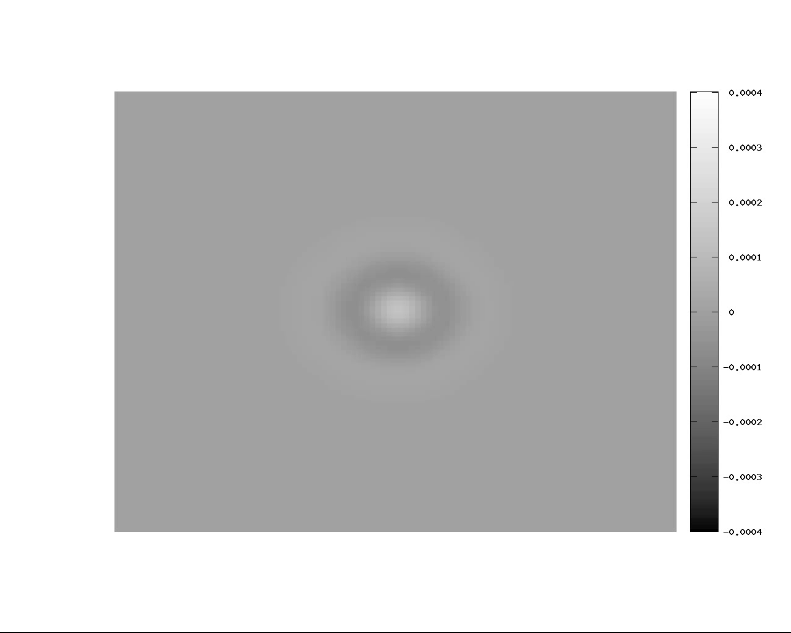
\includegraphics[width=8cm,trim=0 4mm 0 0,clip]{delta_drop_exp_bottom1.png}
    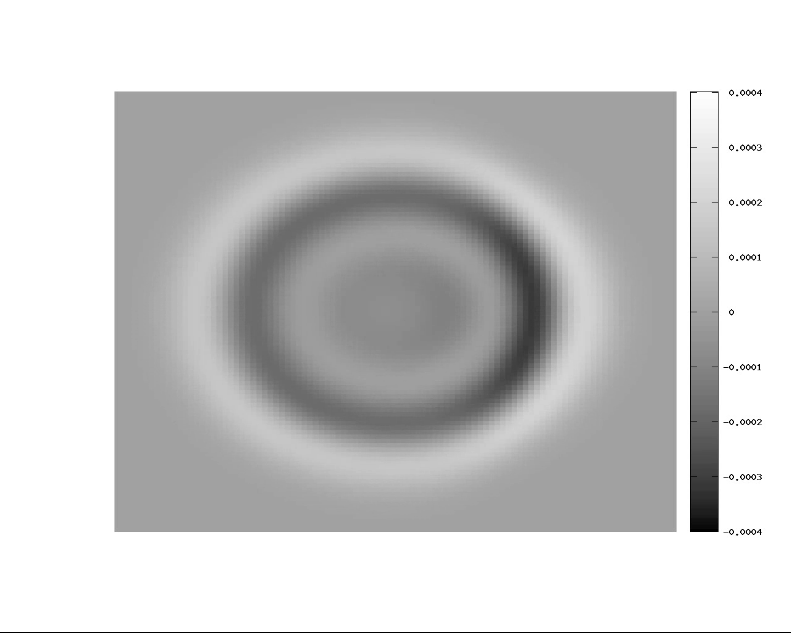
\includegraphics[width=8cm,trim=0 4mm 0 0,clip]{delta_drop_exp_bottom2.png}
    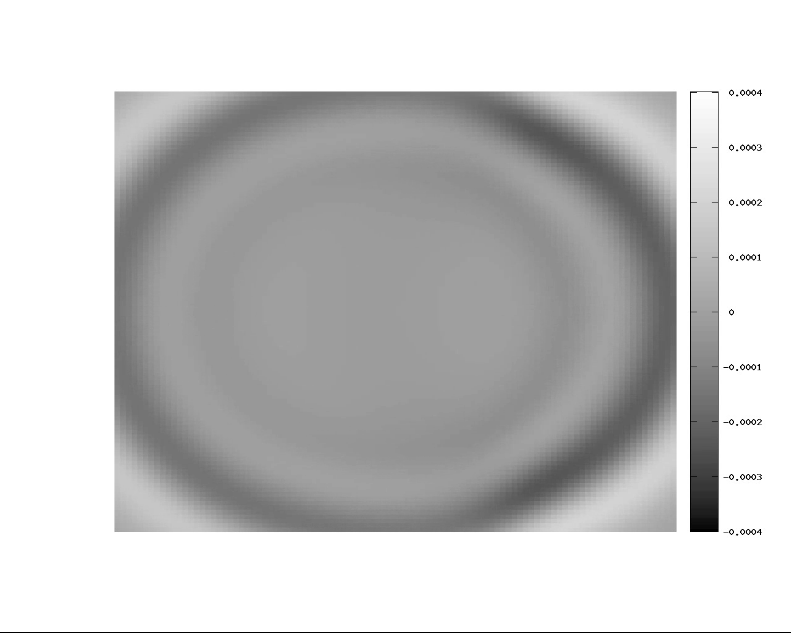
\includegraphics[width=8cm,trim=0 4mm 0 0,clip]{delta_drop_exp_bottom3.png}
    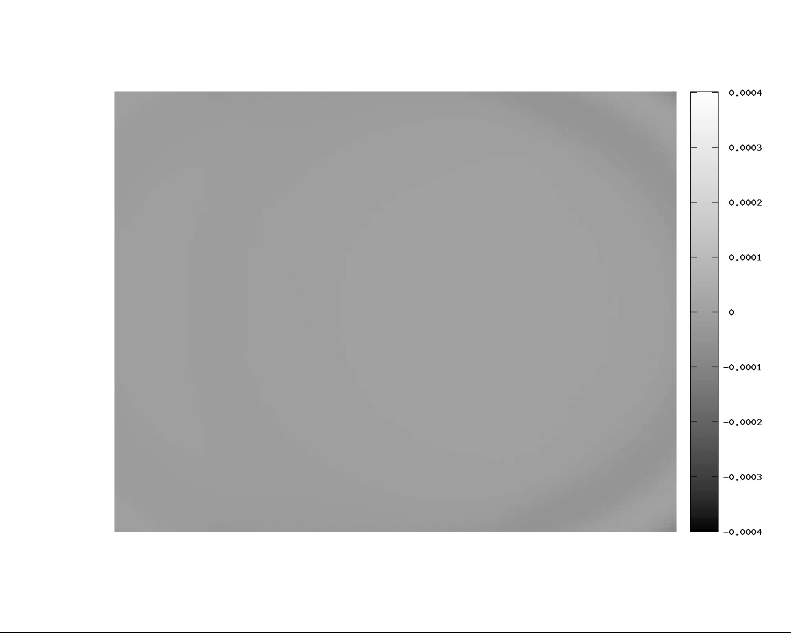
\includegraphics[width=8cm,trim=0 4mm 0 0,clip]{delta_drop_exp_bottom4.png}
    \caption{Динамика разности расчетов в линейном и нелинейном случае с препятствием у границы на 20, 80, 200 и 380 шаге}
    \label{fig:ExpWaveDelta}
\end{figure}

\newpage
\addtocounter{section}{1}
\setcounter{subsection}{0}
\setcounter{equation}{0}
\section*{Эффект возникновения волны}
\addtocontents{toc}{\contentsline{section}{\protect\numberline{\S\;\thesection.}\vspace{10pt}Эффект возникновения волны}{\thepage}}

В процессе проведения расчетов был обнаружен любопытный эффект, который ранее нигде встречался. Данный эффект достаточно устойчив, для того, чтобы не списать его на ошибки или неточности, поэтому привлек внимание.

После того как волна полностью выходит из расчетной области, в ней остаются некоторые регулярные колебания, волны, амплитуда которых меньше, чем исходная. Если продолжить расчет в этой ситуации, либо взять указанные колебания в качестве начальных данных для нового расчета, то произойдет <<возвращение>> волны - т.е. свободная поверхность начинает изменяться и принимает форму, обратную той, что была задана в качестве начального положения.

\begin{figure}[H]
    \centering
    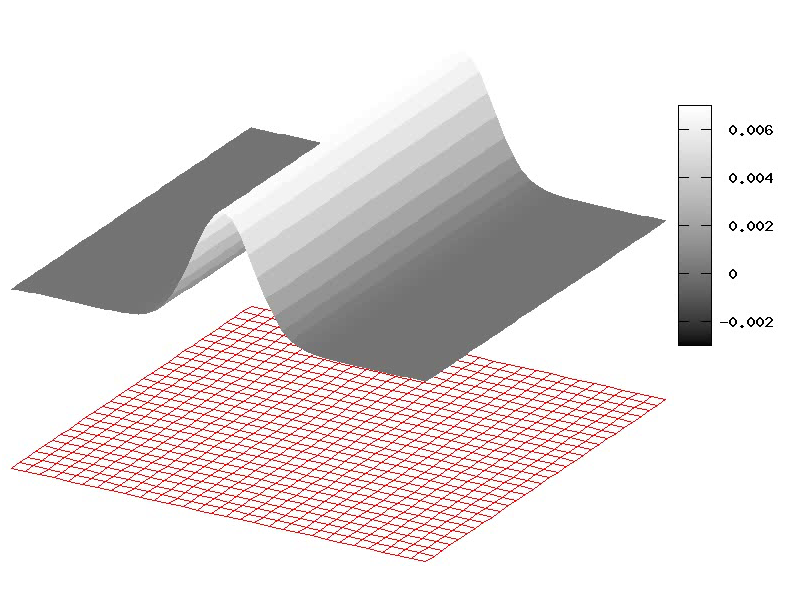
\includegraphics[width=8cm]{simple_return1.png}
    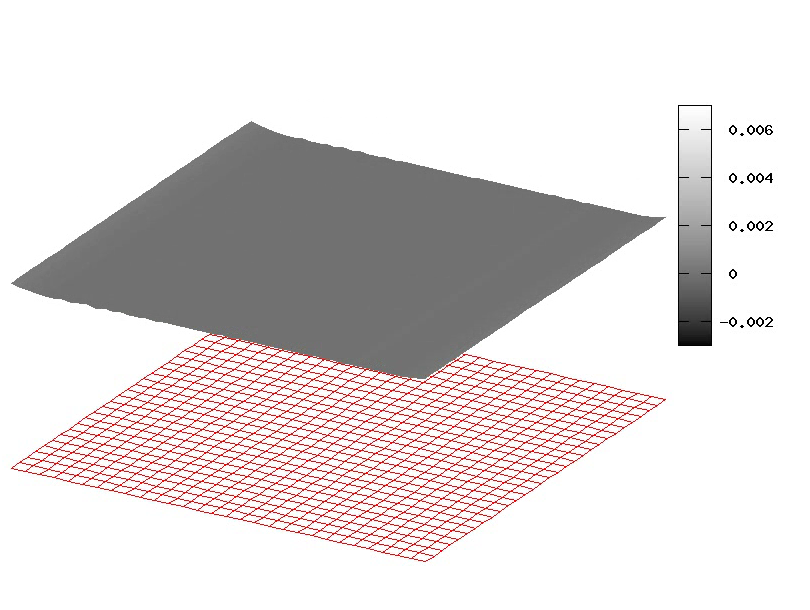
\includegraphics[width=8cm]{simple_return4.png}
    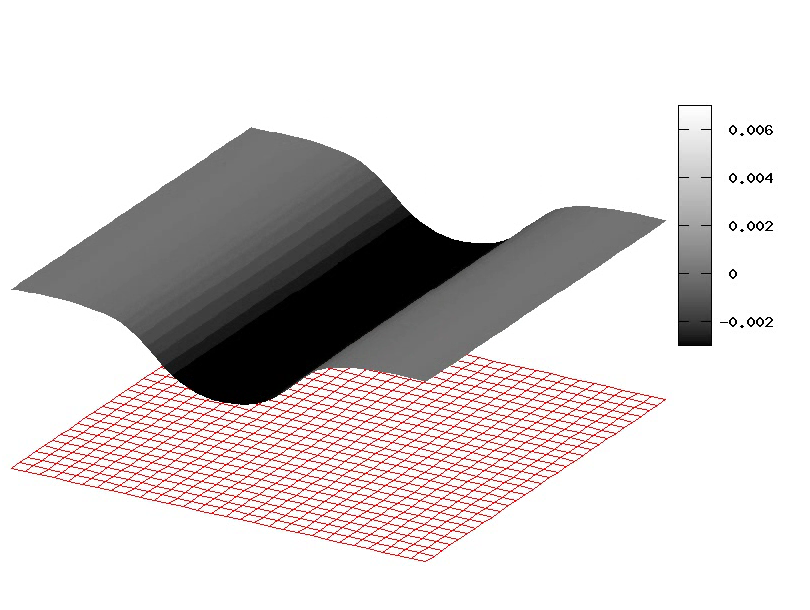
\includegraphics[width=8cm]{simple_return6.png}
    \caption{Графическое представление о возвращенной волне}
    \label{fig:ReturnWaveSmall}
\end{figure}

На рис.\ref{fig:ReturnWave} представлена динамика движения волны следующего вида $u_0=0\;v_0=0\;\eta_0=7 \cdot 10^{-3}e^{(-100 (x-0.5)^2)}$
и ее возвращения. В данном случае произошло возвращение волны с противоположной по знаку амплитуды.

\begin{table}[H]
    \label{tab:FirstResult}
    \caption{Параметры для расчетов с возвращением волны над ровным дном}
    \begin{center}
	\begin{tabular}{|c|c|c|}
	    \hline
	    Размер области & $1\times1$\\
	    \hline
	    Количество шагов & $600$\\
	    \hline
	    Шаг по времени & $0.01$\\
	    \hline
	    Шаг сетки & $0.01$\\
	    \hline
	    Точность метода & $10^{-7}$\\
	    \hline
	    Форма дна & $H(x,y)=0.01$\\
	    & $B(x,y,t)=0$\\
	    \hline
	\end{tabular}
    \end{center}
\end{table}

На рис.\ref{fig:ReturnAfterWave} представлено продолжение расчета с начальных данных, взятых после выхода волны следующего вида $u_0=0\;v_0=0\;\eta_0=7\;\cdot\;10^{-3}e^{(-100\;(x-0.3)^2)}$ из расчетой области.

\begin{table}[H]
    \label{tab:FirstResult}
    \caption{Параметры для расчетов с продолженным движением волны над ровным дном}
    \begin{center}
	\begin{tabular}{|c|c|c|}
	    \hline
	    Размер области & $1\times1$\\
	    \hline
	    Количество шагов & $300$\\
	    \hline
	    Шаг по времени & $0.001$\\
	    \hline
	    Шаг сетки & $0.01$\\
	    \hline
	    Точность метода & $10^{-7}$\\
	    \hline
	    Форма дна & $H(x,y)=0.01$\\
	    & $B(x,y,t)=0$\\
	    \hline
	\end{tabular}
    \end{center}
\end{table}

По мере исследования выяснилось, что возвращенная волна может быть в точности такой, как и изначальная, а может иметь меньшую/большую длину. Более того, задание в качестве начальных данных <<колебательного фона>> разных видов (например, произволные колебания маленькой амплитуды, либо колебания, задаваемые по определенной формуле) тоже приводит к появлению некоторых волн. Общим остается тенденция к образованию из небольшого <<колебательного фона>> волн, амплитуда которых на несколько порядков больше (в наших расчетах чаще всего на два порядка).

\newpage
\begin{figure}[H]
    \centering
    \vspace{12em}
    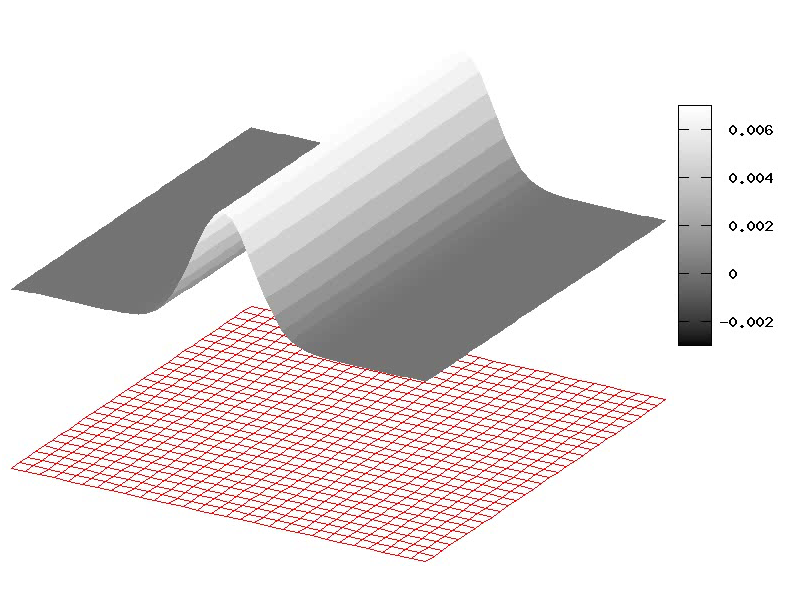
\includegraphics[width=8cm]{simple_return1.png}
    \includegraphics[width=8cm]{simple_return2.png}
    \includegraphics[width=8cm]{simple_return3.png}
    \includegraphics[width=8cm]{simple_return4.png}
    \includegraphics[width=8cm]{simple_return5.png}
    \includegraphics[width=8cm]{simple_return6.png}
    \caption{Динамика движения волны в нелинейном случае на нулевом, 80, 160, 250, 400 и 460 шагах}
    \label{fig:ReturnWave}
\end{figure}

\newpage
\begin{figure}[H]
    \centering
    \vspace{12em}
    \includegraphics[width=8cm]{return_after_wave1.png}
    \includegraphics[width=8cm]{return_after_wave2.png}
    \includegraphics[width=8cm]{return_after_wave3.png}
    \includegraphics[width=8cm]{return_after_wave4.png}
    \includegraphics[width=8cm]{return_after_wave5.png}
    \includegraphics[width=8cm]{return_after_wave6.png}
    \caption{Динамика продолженного движения волны в нелинейном случае на нулевом, 500, 1000, 1500, 2000 и 2500 шагах}
    \label{fig:ReturnAfterWave}
\end{figure}

\newpage
\addtocounter{subsection}{1}
\subsection*{Зависимость от параметров}
\addtocontents{toc}{\contentsline{subsection}{\protect\numberline{\thesubsection.}\vspace{10pt}Зависимость от параметров}{\thepage}}

Была предпринята попытка выяснить причину возникновения такого эффекта с помощью проведения серии расчетов, в которых изменялись бы основные параметры, такие как шаг по пространству, шаг по времени, точность вычислений, начальные данные, параметры, входящие в систему уравнений - т.е. глубина дна $H(x,y)$.

В таблице \ref{tab:Variables} представлены результаты расчетов и указаны следующие параметры: размер сетки, шаг по времени, соотношение $h$ к $\tau$ и результат, который может быть одним из двух - волна возвращается либо нет.

Если в таблице указаны два расчета с одинаковыми параметрами, но разным результатом, это значит, что другие параметры, не отраженные в таблице, были различными (точность вычислений, начальные данные).

\begin{table}[p]
    \caption{Результаты расчетов с различными параметрами}
    \label{tab:Variables}
    \begin{center}
	\begin{tabular}{|c|c|c|c|}
	    \hline
	    Размер сетки & Соотношение $h \tau$ & Шаг по времени & Результат\\
	    \hline
	    100x100 & $1.0101\ldots$ & 0.01 & не возвращается\\
	    \hline
	    100x100 & $1.0101\ldots$ & 0.01 & не возвращается\\
	    \hline
	    100x100 & 1.0101... & 0.01 & возвращается\\
	    \hline
	    50х50 & 20,4081632 & 0.001 & возвращается\\
	    \hline
	    50х50 & 2,04081632 & 0.01 & не возвращается\\
	    \hline
	    150х150 & 0,67114093 & 0.01 & не возвращается\\
	    \hline
	    150х150 & 0,67114093 & 0.01 & возвращается\\
	    \hline
	    100х100 & 1.0101... & 0.01 & возвращается\\
	    \hline
	    100х100 & 1.0101... & 0.01 & возвращается\\
	    \hline
	    200х200 & 0,50251256 & 0.01 & не возвращается\\
	    \hline
	    200х200 & 5,0251256 & 0.001 & возвращается\\
	    \hline
	    50х50 & 2,04081632 & 0.01 & не возвращается\\
	    \hline
	    50х50 & 20,4081632 & 0.001 & возвращается\\
	    \hline
	    50х50 & 40,963264 & 0.0005 & возвращается\\
	    \hline
	    50х50 & 20,4081632 & 0.001 & возвращается\\
	    \hline
	    50х50 & 2,04081632 & 0.01 & не возвращается\\
	    \hline
	    50х50 & 0,204081632 & 0.1 & не возвращается\\
	    \hline
	    50х50 & 40,8163264 & 0.0005 & возвращается\\
	    \hline
	    50х50 & 4,08163264 & 0.005 & возвращается\\
	    \hline
	    50х50 & 0,408163264 & 0.05 & не возвращается\\
	    \hline
	    50х50 & 0,408163264 & 0.05 & не возвращается\\
	    \hline
	    100х100 & 0,20202... & 0.05 & не возвращается\\
	    \hline
	    100х100 & 1,0101... & 0.01 & не возвращается\\
	    \hline
	    100х100 & 1,0101... & 0.01 & возвращается\\
	    \hline
	\end{tabular}
    \end{center}
\end{table}

Графическое представление этих данных дает некоторое представление о зависимостях между параметрами и результатом.
На рис.\ref{fig:VariablesGraph} изображены характеристики \nocite{yanenko} уравнения, которое описывает движение волны $\frac{\partial x}{\partial t}=g\;\frac{\partial x}{\partial t}=H $, где $H$ - постоянная часть дна (в данных расчетах $H=0.1$). На графике точками указаны проведенные расчеты, в соответствии с отношением $h$ к $\tau$ . Кругами отмечены расчеты, в которых волна возвращается, квадратами - в которых волна не возвращается.

\begin{figure}[H]
    \centering
    \includegraphics[height=8cm]{variables.png}
    \caption{Графическое представление данных о возвращении}
    \label{fig:VariablesGraph}
\end{figure}

\newpage
В результате такого представления были сделать предположение о причинах возникновения эффекта возвращения:
\begin{itemize} 
    \item если соотношение $h$ и $\tau$ больше, чем верхняя характеристика ($g$), то волна всегда возвращается.
    \item Если меньше - то возвращение зависит от других параметров.
    \item В области ниже характеристики $H$  расчетов нет, но близкие к ним (соотношение $h$ и $\tau$ примерно $0.2$) характеризуются тем, что волна в них почти никогда не возвращается. Помимо этого можно отметить тот факт, что в тех расчетах, где волна возвращалась, при увеличении $H$ волна переставала возвращаться. В связи с этим можно предположить, что все расчеты, соотношение $h$ и $\tau$ в которых меньше нижней характеристики ($H$), характеризуются тем, что волна не возвращается
\end{itemize}

\addtocounter{subsection}{1}
\subsection*{Расчет с начальных данных}
\addtocontents{toc}{\contentsline{subsection}{\protect\numberline{\thesubsection.}\vspace{10pt}Расчет с начальных данных}{\thepage}}

В качестве интересного результата были получены начальные данные небольшой <<нулевой>> амплитуды, при подстановке которых в расчет наблюдается появление движущейся в области волны. Т.о. более правильно говорить не о <<возвращении>>, а о <<возникновении>> волны на поверхности жидкости, что приводит к мысли о возможности моделирования такого явления, как <<волна-убийца>>.

\begin{table}[H]
    \label{tab:FirstResult}
    \caption{Параметры для расчетов с возникновением волны}
    \begin{center}
	\begin{tabular}{|c|c|c|}
	    \hline
	    Размер области & $1\times1$\\
	    \hline
	    Количество шагов & $2000$\\
	    \hline
	    Шаг по времени & $0.001$\\
	    \hline
	    Шаг сетки & $0.01$\\
	    \hline
	    Точность метода & $10^{-4}$\\
	    \hline
	    Форма дна & $H(x,y)=0.1\;B(x,y,t)=0$\\
	    \hline
	\end{tabular}
    \end{center}
\end{table}

На рис.\ref{fig:ReturnMoveWave} представлена динамика движения такой волны.

\newpage
\begin{figure}[H]
    \centering
    \vspace{12em}
    \includegraphics[width=8cm,trim=0 4mm 0 0,clip]{return_move_wave1.png}
    \includegraphics[width=8cm,trim=0 4mm 0 0,clip]{return_move_wave2.png}
    \includegraphics[width=8cm,trim=0 4mm 0 0,clip]{return_move_wave3.png}
    \includegraphics[width=8cm,trim=0 4mm 0 0,clip]{return_move_wave4.png}
    \caption{Движение волны с <<нулевого фона>> на 200, 700, 1200 и 1600 шагах}
    \label{fig:ReturnMoveWave}
\end{figure}

\newpage
\addtocounter{section}{1}
\setcounter{subsection}{0}
\setcounter{equation}{0}
\section*{Выводы} 
\addtocontents{toc}{\contentsline{section}{\protect\numberline{\S\;\thesection.}\vspace{10pt}Выводы}{\thepage}}

Проанализировав представленные расчеты, можно сделать несколько выводов:
\begin{itemize}
    \item Предлагаемый подход к решению задачи (\ref{eq:MainVectorForm})-(\ref{eq:BoundaryCondition}) с использованием неявных схем и аппроксимации исходной системы уравнений на границе конечной области позволяет находить в ней решение без отражений или искажений. Для всех случаев (сложная начальная форма свобожной поверхности, неровное дно, линейная и нелинейная форма уравнения) было получено решение, соответствующее реальным физическим представлениям о задаче, возмущения свободной поверхности безпрепятственно выходили из области, при этом не искажаясь и не порождая отражений.
    \item Расчет в линейном и нелинейном случае показал, что нелинейная форма уравнений (\ref{eq:MainVectorForm})-(\ref{eq:BoundaryCondition}) приводит к тому, что волны свободной поверхности со временем меняют свою форму, становятся менее симметричными относительно своего центра.
	\begin{figure}[H]
	    \centering
	    \includegraphics[width=8cm]{Lin.png}
	    \includegraphics[width=8cm]{Nonlin.png}
	    \caption{Форма волны в линейном(слева) и нелинейном(справа) случае}
	    \label{fig:Lin_Nonlin_Wave}
	\end{figure}
	Для нелинейных уравнений за основной волной формируются вторичные колебания, амплитуда которых много меньше исходной. При этом указанные эффекты со временем проявляются все более сильно.
\end{itemize}

\newpage
\addtocounter{chapter}{1}
\setcounter{section}{0}
\setcounter{figure}{0}
\setcounter{table}{0}
\setcounter{equation}{0}
\diplomchapter*{Приложения}
\addtocontents{toc}{\contentsline{chapter}{\protect\numberline{Глава \thechapter.}\vspace{10pt}Приложения}{\thepage}}

\setcounter{figure}{0}
\setcounter{table}{0}
\setcounter{equation}{0}
\setcounter{subsection}{0}
\addtocounter{section}{1}
\section*{Программные средства}
\addtocontents{toc}{\contentsline{section}{\protect\numberline{\S\;\thesection.}\vspace{10pt}Программные средства}{\thepage}}
Для проведения расчетов была написан программный комплекс, позволяющий эффективно решать поставленную задачу и ряд сопутствующих проблем. Его разработка велась на языке программирование C++ с использованием компилятора из GNU Compiler Collection и системы автоматизации сборки программного обеспечения из исходного кода CMake. Для решения некоторых задач использовались сторонние инструменты. Так, для пофилирования использовались Valgrind и AMD CodeAnalyst, для визуализации полученных данных - Gnuplot, для генерации документации - Doxygen. Разработка велась под управлением системы контроля версий Git, исходный код был расположен в репозитории code.google.com под академической лицензией MIT.

Написанный программный комплекс	реализует алгоритмы, описанные в предыдущих разделах, и позволяет моделировать движение свободной поверхности жидкости при различных условиях. Моделирование может происходить на основе линейных или нелинейных уравнений, с разными начальными данными, параметрами расчетов и формой дна.

Изменяемыми являются:
\begin{itemize}
    \item начальное значение свободной поверхности
    \item начальное значение распределения скоростей
    \item уравнение, описывающее статическую часть дна
    \item уравнение, описывающее динамическую часть дна
    \item параметры расчетной области
    \item параметры численного метода
    \item значение шага по времени и продолжительность моделирования
\end{itemize}

В процессе работы программного комплекса формируются файлы, содержащие расчетные данные. Они полностью описывают итоговое распределение скоростей и положение свободной поверхности на каждом временном шаге. Помимо этого, можно выполнить сравнение полученных результатов и также получить файл с данными, описывающими отличия.

Все расчетные данные могут быть визуализированы в двух основных представлениях - с учетом дна и в проекции сверху.

\addtocounter{subsection}{1}
\setcounter{equation}{0}
\subsection*{Решенные задачи}
\addtocontents{toc}{\contentsline{subsection}{\protect\numberline{\thesubsection.}\vspace{10pt}Решенные задачи}{\thepage}}

В рамках разработки расчетного программного комплекса были решены некоторые проблемы:

\addtocounter{subsubsection}{1}
\subsubsection*{Гибкость и документирование}
\addtocontents{toc}{\contentsline{subsubsection}{\protect\numberline{\thesubsubsection.}\vspace{10pt}Гибкость и документирование}{\thepage}}

Для гибкого конфигурирования и кросплатформенности для сборки проекта были выбраны компилятор g++ из состава GCC, а также система автоматической сборки Cmake. Данные инструменты могут быть использованы на любой платформе, а также поддерживают достаточно удобное управление компиляцией с помощью разнообразных ключей, которые подробно описаны в документации к соответствующим инструментам.

Чтобы улучшить понимаемость исходного кода был использован генератор документации Doxygen. Соответствующим образом был доработан проект, в него были добавлены описания всех используемых классов и методов, а также формат генерируемой документации. В итоге получено достаточно полное описание кода в виде связанных html страниц, которое поможет разработчику гораздо легче разобраться в проекте.

\addtocounter{subsubsection}{1}
\subsubsection*{Визуализация расчетных данных}
\addtocontents{toc}{\contentsline{subsubsection}{\protect\numberline{\thesubsubsection.}\vspace{10pt}Визуализация расчетных данных}{\thepage}}

В качестве инструмента для визуализации расчетных данных был выбран Gnuplot, т.к. он позволяет задавать параметры и способ визуализации с помощью скриптов. Это позволяет достаточно легко сформировать сложную 3d композицию на основе расчетных данных, в которой каждый элемент легко может быть настроен необходимым образом. Результатом работы Gnuplot является gif файл, который в дальнейшем преобразуется в видео файл с помощью выбранного кодека (mpeg2 для совместимости или mpeg4 для лучшего отображения).

Помимо этого была написана небольшая утилита для конвертирования результатов, отформатированных для Tecplot, в формат Gnuplot.

На листинге (\ref{lst:create_animation}) представлено тело скрипта, использованного для визуализации.


\begin{lstlisting}[language=bash,caption=Пример скрипта для визуализации,label={lst:create_animation}]
#!/bin/bash
MAX=$4
echo "clear" >> $1
echo "reset" >> $1
echo "set terminal gif animate delay 10 giant size 1280,1024" >> $1
echo "set palette defined (0 \"black\", 0.001 \"blue\", 0.004 \"green\",0.006 \"yellow\",0.007 \"red\")" >> $1
#echo "set pal gray" >> $1
echo "set output \""$2"\"" >> $1
echo "unset xtics">>$1
echo "unset ytics">>$1
echo "unset ztics">>$1
echo "unset border">>$1

echo "set xrange [0:1]" >> $1
echo "set yrange [0:1]" >> $1
echo "set zrange [-0.011:0.007]" >> $1
echo "set cbrange[-0.003:0.007]" >> $1
for i in `seq 0 ${MAX}`
do
echo "set multiplot" >> $1
echo "set size 0.7,0.7" >> $1
echo "set origin 0.15,-0.15" >> $1
echo "set view 90,0" >> $1
echo "splot \""h.dat"\" with lines t \"\",\""$3"\" index $i using 1:2:3 with pm3d t \"\"" >> $1

echo "set size 0.7,0.7" >> $1
echo "set origin 0.15,0.35" >> $1
echo "set view 60,30" >> $1
echo "splot \""h.dat"\" with lines t \"\",\""$3"\" index $i using 1:2:3 with pm3d lc rgb \"black\" t \"\"" >> $1

echo "unset multiplot" >> $1
done
\end{lstlisting}

\addtocounter{subsubsection}{1}
\subsubsection*{Оптимизация времени работы}
\addtocontents{toc}{\contentsline{subsubsection}{\protect\numberline{\thesubsubsection.}\vspace{10pt}Оптимизация времени работы}{\thepage}}

В процессе разработки часть усилий была протрачена на оптимизацию программы. Увеличение производительности происходило 2-мя путями:
\begin{itemize}
    \item Выявление ненужных действий и <<узких>> мест в программной реализации алгоритма
    \item Использование возможностей компилятора. Были проанализированы различные настройки компилятора gcc и их влияние на производительность генерируемого кода. Здесь стоит отметить, что современные компиляторы ориентированы на создание более универсальных программ, поэтому добавляют в генерируемый машинный код некоторое количество полезного в общем случае функционала. Но расчетные программы являются узкоспециализированными и не нуждаются в нем, соответственно, отключая данные возможности можно оптимизировать по скорости получаемый код.
\end{itemize}

Оба вида оптимизации не затрагивали алгоритм решения задачи, т.е. неоптимизированный код эквивалентен оптимизированному.

\begin{table}[H]
    \label{tab:CXXFLAGS}
    \caption{Используемые флаги компиляции}
    \begin{center}
    \large{
	\begin{tabular}{|p{0.3\linewidth}|p{0.5\linewidth}|}
	    \hline
	    Ключ & Описание\\
	    \hline
	    o3 & Наивысший уровень оптимизации(компилятор выбирает почти все опции, позволяющие генерировать быстрый код)\\
	    \hline
	    march=native & Указывает компилятору определить тип процессора и оптимизировать код для него\\
	    \hline
	    ffast-math (либо только funsafe-math-optimization) & Устанавливает режим <<быстрой математики>> для программ, в которых не требуется точной реализации IEEE/ISO стандартов для математических функций\\
	    \hline
	    fomit-frame-pointer & Разрешает не хранить в регистрах указатель на фрейм для функции, которая больше не используется (эта опция уже включена в o3, но иногда явное ее указание заметно улучшает производительность)\\
	    \hline
	    fno-stack-protector & Убирает проверку целостности стека после выхода из функции\\
	    \hline
	    fprefetch-loop-array & Генерирует инструкции для предварительной выборки в циклах с большими массивами (если позволяет архитектура целевой машины)\\
	    \hline
	    funsafe-loop-optimizations & Указывает, что циклы в программе не переполняются и не являются бесконечными, что позволяет сгенерировать более быстрый код\\
	    \hline
	    funroll-loops & Позволяет раскрыть циклы, размер которых может быть вычислен на этапе компиляции\\
	    \hline
	    mpreferred-stack-boundary=num & Указывает выравнивание для стека и в некоторых случаях влияет на скорость (по умолчанию num=2, в случае данной программы наибольшая скорость выполнения была получена при num=6)\\
	    \hline
	    ftracer & Форсирует хвостовую дубликацию, делая управление потоком выполнения более простым\\
	    \hline
	\end{tabular}
	}
    \end{center}
\end{table}

К возможностям компилятора также относится и компиляция с обратной связью (Profile-guided optimization). В отличие от традиционных способов оптимизации анализирующих исключительно исходные коды, PGO использует результаты измерений тестовых запусков оптимизируемой программы для генерации более оптимального кода. Тестовые запуски выявляют какие части программы исполняются чаще, а какие реже. Преимущество такого подхода в том что компилятор не строит предположений при выборе способа оптимизации, а использует реальную статистику, собранную во время выполнения программы. В силу специфики расчетных программ данный вид оптимизации оказывается достаточно действенным. Техники оптимизации PGO реализованы, во многих компиляторах, в частности: Intel C++ Compiler, Inter Fortran Compiler, GCC, Sun Studio, Microsoft Visual C++, поэтому они могут быть использованы практически в любом расчетном проекте вне зависимости от платформы.

Пример использования техники PGO для gcc выглядит следующим образом:

\begin{lstlisting}[language=bash,caption=Пример компиляции для сбора статистики,label={lst:profile_generate}]
g++ -O3 -fprofile-generate -c -fmessage-length=0 -MMD -MP -MF program.d -MT program.d -o program.o program.cpp

g++ -fprofile-generate -o program ./program.o
\end{lstlisting}

Для сбора статистики используется ключ {\bf fprofile-generate}, а результатом компиляции являются объектные файлы. Затем тот же ключ необходимо отдельно указать линковщику. Полученная в итоге программа будет работать медленнее, т.к. собирает статистику о действиях программы, которая затем будет помещена в файл с расширением {\bf *.gcda}.

После этого необходимо вновь скомпилировать программу, но уже с учетом набранной статистики - для этого аналогичным образом используется флаг {\bf fprofile-use}.

\begin{lstlisting}[language=bash,caption=Пример компиляции с учетом статистики,label={lst:profile_use}]
g++ -O3 -fprofile-use -c -fmessage-length=0 -MMD -MP -MF program.d -MT program.d -o program.o program.cpp

g++ -fprofile-use -o program ./program.o
\end{lstlisting}

\newpage
\addtocounter{subsection}{1}
\setcounter{equation}{0}
\subsection*{Сервер вычислений}
\addtocontents{toc}{\contentsline{subsection}{\protect\numberline{\thesubsection.}\vspace{10pt}Сервер вычислений}{\thepage}}

Моделирование движения жидкости с помощью разработанной программы требует выполнения последовательности действий и вовлечения в процесс обработки некоторых инструментов. Это, например, сборка программы с изменениями, внесенными в алгоритм, запуск программы с определенными параметрами, визуализация полученных данных. В обычном случае многие из этих действий выполняются исследователем вручную. Для облегчения работы было создано небольшое приложение (<<сервер вычислений>>), которое позволяет объединить необходимые для моделирования действия в рамках одной среды, а также делает работу более удобной.

Требования, которые могут предъявляться к серверу:
\begin{itemize}
	\item Сборка и выполнение расчетной программы
	\item Управление запущенными программами
	\item Пост- и преобработка результатов
	\item Управление файлами и хранение информации, описывающей расчет
	\item Загрузка полученных результатов
\end{itemize}

Основные принципы, используемые в процессе его разработки:
\begin{itemize}
    \item Объединение различных процессов, составляющих проведение расчета
    \item Создание <<обертки>> вокруг уже существующего кода
    \item Гибкость доступа и работы с процессами расчета (запуск,получение информациио состоянии запущенных задач, отмена задачи и т.д.)
    \item Легкая адаптируемость под разные задачи
\end{itemize}

<<Сервер вычислений>> представляет собой TCP сервер, написанный на скриптовом языке python. В нем заложен общий алгоритм проведения расчета, каждый конкретный этап которого реализуется отдельным модулем. Т.о. реализуется шаблон <<стратегия>>, и достигается высокий уровень гибкости, т.к. python позволяет создавать новые модули в замен старых без необходимости создания структуры интерфейсов и изменения исходного кода.

Сервер принимает сообщения в формате xml, описывающие команды к выполнению. Например, запустить указанную программу с выбранными параметрами, что позволяет достаточно легко адаптировать сервер к новым задачам.

При этом на исходный код расчетной программы не накладывается практически никаких ограничений. Сервер просто запускает ее и анализирует результат ее работы, получаемый из стандартного потока вывода. Т.о. например, реализована возможность отслеживания состояния запущенной программы, тогда как, например, во многих планировщиках задач, испольуемых на вычислительных кластерах (Altair PBS), эта информация недоступна.

На данный момент реализован основной функционал сервера вычислений, позволяющий использовать его в работе. Написаны модули, позволяющие производить предварительную обработку кода программы - компиляцию с помощью GCC и утилиты Make, и визуализировать результаты с использованием Gnuplot.

\newpage
\listoffigures
\addtocounter{section}{1}
\addtocontents{toc}{\contentsline{section}{\protect\numberline{\S\;\thesection}\vspace{10pt}Список иллюстраций}{\thepage}}

\newpage
\listoftables
\addtocounter{section}{1}
\addtocontents{toc}{\contentsline{section}{\protect\numberline{\S\;\thesection}\vspace{10pt}Список таблиц}{\thepage}}

\newpage
\bibliography{lib}
\addcontentsline{toc}{chapter}{Литература}
\end{document}
